\documentclass[11pt]{amsart}

% Encoding and fonts
\usepackage[T1]{fontenc}
\usepackage[utf8]{inputenc}
\usepackage{lmodern}

% Math packages
\usepackage{amsmath}
\usepackage{amssymb}
\usepackage{amsfonts}
\usepackage{amsthm}
\usepackage{mathtools}

% Layout and utilities
\usepackage{geometry}
\usepackage{enumitem}
\usepackage{booktabs}
\usepackage{graphicx}
\geometry{margin=1in}
\raggedbottom

\numberwithin{equation}{section}
\setcounter{tocdepth}{3}
\setcounter{secnumdepth}{3}

% Theorem-like environments
\theoremstyle{plain}
\newtheorem{theorem}{Theorem}[section]
\newtheorem{proposition}[theorem]{Proposition}
\newtheorem{lemma}[theorem]{Lemma}
\newtheorem{corollary}[theorem]{Corollary}
\newtheorem{conjecture}[theorem]{Conjecture}

\theoremstyle{definition}
\newtheorem{definition}[theorem]{Definition}
\newtheorem{experiment}[theorem]{Experiment}
\newtheorem{heuristic}[theorem]{Heuristic}
\newtheorem{question}[theorem]{Question}

\theoremstyle{remark}
\newtheorem{remark}[theorem]{Remark}
\newtheorem{warning}[theorem]{Warning}

\newcommand{\mob}{\mu}
\newcommand{\Mert}{M}
\newcommand{\Sq}{Q}
\newcommand{\PS}{\mathcal P}

\title{An Ordinal-Prime Transform of the M\"obius Function}
\author{}
\date{Version 12 --- 7 September 2026}

% hyperref must be loaded last
\usepackage[hidelinks]{hyperref}
\begin{document}

\maketitle
\enlargethispage{2pt}
\tableofcontents

\section{Purpose and scope}
\label{sec:purpose}

This note develops the ordinal-prime transform of the M\"obius function and
determines exactly how much arithmetic information it carries. It is
self-contained and uses no other construction.

The starting point is the M\"obius function $\mob(n)\in\{-1,0,+1\}$. The
occurrences of $-1$ and of $+1$ are numbered separately, in increasing order of
$n$, and the corresponding ordinal prime is attached to each occurrence; zeros
are mapped to $1$. The resulting signed sequence is $S(n)$ and its partial sum
is $SS(n)=\sum_{k\le n}S(k)$.

The conclusions are:

\begin{enumerate}[label=(\roman*)]
\item $SS(n)$ has an exact closed form in terms of the Mertens function
$\Mert(n)$, the squarefree counting function $\Sq(n)$, and the sum of the first
$m$ primes (Proposition~\ref{prop:closed}).
\item After subtracting the deterministic zero contribution $n-\Sq(n)$, the
remainder $T(n):=SS(n)-n+\Sq(n)$ is \emph{exactly} a signed sum of $|\Mert(n)|$
consecutive primes, occupying a window of prime indices symmetric about
$(\Sq(n)+1)/2$ (Proposition~\ref{prop:block}).
\item Consequently $T(n)=\Mert(n)\,p_{\lfloor \Sq(n)/2\rfloor}(1+\theta(n))$
with $\theta(n)\to0$ effectively, and the Mertens criterion transfers to $T$ in
both directions (Theorem~\ref{thm:RH}).
\item Every endpoint object built in Sections~\ref{sec:transform}--\ref{sec:gap-representation} --- $SS$, $T$, the residual $E$, and the centered
residual $E_{\mathrm{mid}}$ --- is a deterministic function of the pair
$(\Mert(n),\Sq(n))$ alone. The transform therefore creates no independent
arithmetic constraint on $\Mert(n)$. This applies to the residuals as well and
is stated as Proposition~\ref{prop:info}.
\item The nonlinearity of the transform splits exactly into a central part
linear in $\Mert(n)$ and an \emph{antisymmetric weighted sum of prime gaps}
with triangular weights (Theorem~\ref{thm:gaps}). The weight norm has a closed
form (Lemma~\ref{lem:w2}), which forces the exponent $3/2$ in the observed law
$|E_{\mathrm{mid}}(n)|\approx0.155\,|\Mert(n)|^{3/2}\log n$.
\item The measured size of that residual is quantitatively accounted for by the
local covariance structure of prime gaps. A covariance-corrected model predicts
its standard deviation to within $0.3\%$ with no free parameter, whereas an
independent-gap model overpredicts it, the observed-to-predicted ratio being
$0.853$
(Section~\ref{sec:numeric}, part D).
\item The packet structure visible in $E_{\mathrm{mid}}$ is an amplitude effect:
its moving RMS follows $|M(n)|^{3/2}\log n$. On the logarithmic coordinate
$u=\log n$, the spectrum of $M(e^u)e^{-u/2}$ displays the ordinates $\gamma_k$
of zeta zeros, as predicted by the classical explicit formula. This spectral
observation is a sanity check, not new information about the zeros; the finite
$u$-window has frequency resolution about $0.91$.
\item A separate test asks whether the prime-gap fluctuation factor is coupled to
the sign or zeta phase of $M$. No such coupling is detected at the present
scale. With effective sample about $1.7\times10^4$, the tests only exclude
linear effects larger than roughly $0.015$ and do not constitute a theorem of
independence.
\item Versions 7--9 introduce the inverse-counting displacement
$d_j=\beta_j-\alpha_j$.  Its logarithmic two-point squarefree-time correlation
has an unconditional theorem, but several apparently stronger uses are shown
to collapse: odd parity is an involutive algebraic cancellation rather than a
Mertens bound; a universal coercive functional can be evenised; a simple
real-axis lower bound for its generating function fails by an exact finite
counterexample; and the natural two-cut survival kernel depends only on the
two endpoint heights.
\item Version 9 proves a square-root recovery theorem: the genuine prefix
$SS(0),\ldots,SS(\lfloor\sqrt N\rfloor)$ together with the endpoint $SS(N)$
determines $Q(N)$ and then $M(N)$ uniquely.  The theorem is a recovery identity,
not a cryptographic authentication statement: an independent verifier must still
check that the decoded short prefix is the actual M\"obius function.
\item Version 9 also studies the self-map $\varphi(n)=|S(n)|$ on the squarefree
integers.  Its functional digraph is classified exactly: the first ten primes
$2,3,\ldots,29$ are the only periodic points and are fixed; every other
squarefree input reaches a prime at least $31$ after one step and then increases
strictly to infinity.  On prime indices the map is
$f(j)=N_-(p_j)=j+C_-(p_j)$, is strictly increasing, and its image has counting
function asymptotic to $(\pi^2/3)J/\log J$; hence a density-one set of prime
indices starts escaping rays.  Escaping orbits satisfy an unconditional prime-
number-theorem growth law.
\item Version 11 gives exact formulae for every crossing and every return to a
fixed Mertens level.  Returns to $h>0$ force $SS$ upward, returns to $h=0$
change it by exactly the number of intervening nonsquarefree integers, and
returns to $h<0$ contain a strictly positive prime-separation deficit.
\item For a complete negative squarefree excursion of depth $H$, the sum
$\mathcal A$ of these prime-separation deficits satisfies the unconditional
coercive inequality
$\mathcal A\ge (H^3-H)/3$.  This is a genuine one-sided use of the negative
levels, although an independent upper bound for $\mathcal A$ would still be
needed to deduce a new bound for $M$.
\item Version 11 separates position, ordinal growth, and primality exactly.
Replacing $p_j$ by $j$ gives
$SS_{\rm ord}=n-Q+M(Q+1)/2$, while the genuinely prime contribution is a
signed block of the positive displacements $p_j-j$.  The prime number theorem
then gives an amplitude amplification asymptotic to $\log(Q/2)$ and a squared
energy amplification asymptotic to $\log^2(Q/2)$.
\item Version 12 adds the independent research chapter
Section~\ref{sec:alpha-programme}. It proves the exact Dirichlet decomposition,
two-cut duration identity, and holomorphy of every bounded-duration paired
subseries. It states the unresolved original-order Cauchy condition with its
RH transfer, and compares its precise obligations with established research
programmes. This is a programme with proved intermediate statements, not a
proof of RH or an assertion of universal priority.
\end{enumerate}

The numerical pipeline was regenerated in Python for $1\le n\le10^{6}$ where
stated.  The package contains the scripts, intermediate arrays, textual outputs,
and figure-generation code.  Historical follow-up values from earlier versions
were replaced by the regenerated values whenever the original computation was
not reproducible from a supplied script.

\begin{remark}[Version 5 audit scope]
\label{rem:v5-audit}
Version 12 retains the section-based equation numbering and complete equation labelling
introduced in Version 5. It also retains the boundary and status corrections made there: the
multiplicative prime scale starts at $n=2$; the residuals are not claimed to be
monotone in $M$; prime gaps are not asserted pointwise to be asymptotic to
$\log p$; the cases $|M|\le2$ are separated in the gap formula; the
prime-counting integral includes the $a=0$ endpoint convention; all sums used
in that integral and in the $\kappa$ identity are explicitly finite; the
Montgomery--Soundararajan comparison is identified as a reference scale for
weighted prime counts rather than a theorem about the unweighted $\pi$ count;
and the shared-counter non-endpoint claim is stated as a functional statement
with an explicit pair of histories.
\end{remark}

\section{Notation and elementary lemmas}
\label{sec:notation}

Let $p_1=2,p_2=3,p_3=5,\ldots$ denote the primes in increasing order, and set
$p_0:=0$ by convention (used only to make the product forms below well defined
at $n=1$).

Write
\begin{equation}
\label{eq:basic-definitions}
\Mert(n):=\sum_{k\le n}\mob(k),
\qquad
\Sq(n):=\sum_{k\le n}\mob(k)^2 ,
\qquad
\PS(m):=\sum_{j=1}^{m}p_j ,\quad \PS(0):=0 .
\end{equation}

Define the cumulative occurrence counts
\begin{equation}
\label{eq:occurrence-counts}
N_-(n)=\sum_{k\le n}\frac{\mob(k)^2-\mob(k)}2,
\qquad
N_0(n)=\sum_{k\le n}\bigl(1-\mob(k)^2\bigr),
\qquad
N_+(n)=\sum_{k\le n}\frac{\mob(k)^2+\mob(k)}2 .
\end{equation}
Thus $N_-(n)$, $N_0(n)$, $N_+(n)$ count the occurrences of $\mob=-1$, $\mob=0$,
$\mob=+1$ up to $n$, and the counts are inclusive of $n$ itself.

\begin{lemma}[Counter identities]\label{lem:counters}
For every $n\ge1$,
\begin{equation}
\label{eq:counter-identities}
N_+(n)+N_-(n)=\Sq(n),
\qquad
N_+(n)-N_-(n)=\Mert(n),
\qquad
N_0(n)=n-\Sq(n),
\end{equation}
hence
\begin{equation}
\label{eq:counter-solutions}
N_+(n)=\frac{\Sq(n)+\Mert(n)}2,
\qquad
N_-(n)=\frac{\Sq(n)-\Mert(n)}2 .
\end{equation}
\end{lemma}

\begin{lemma}[Parity]\label{lem:parity}
$\Sq(n)\equiv \Mert(n)\pmod 2$ for every $n\ge1$. Consequently the indices
$(\Sq(n)\pm\Mert(n))/2$ occurring throughout are integers.
\end{lemma}

\begin{proof}
$\Sq=N_++N_-$ and $\Mert=N_+-N_-$, so $\Sq-\Mert=2N_-$.
\end{proof}

Lemma~\ref{lem:parity} is used silently in every subsequent formula and was
absent from version 1; without it the central identities are not well formed.

\section{The transform}
\label{sec:transform}

\begin{definition}
\label{def:transform}
The three rows are
\begin{equation}
\label{eq:transform-rows}
R_-(n)=-\frac{\mob(n)^2-\mob(n)}2\,p_{N_-(n)},
\qquad
R_0(n)=1-\mob(n)^2,
\qquad
R_+(n)=\frac{\mob(n)^2+\mob(n)}2\,p_{N_+(n)} ,
\end{equation}
with the convention $p_0=0$ (needed only at $n=1$, where $N_-(1)=0$ and the
coefficient vanishes). The ordinal-prime transform is
\begin{equation}
\label{eq:transform-piecewise}
S(n):=R_-(n)+R_0(n)+R_+(n)
=
\begin{cases}
-p_{N_-(n)},&\mob(n)=-1,\\[1mm]
1,&\mob(n)=0,\\[1mm]
+p_{N_+(n)},&\mob(n)=+1 .
\end{cases}
\end{equation}
\end{definition}

Along the occurrences of $\mob=-1$ the values are $-2,-3,-5,-7,-11,\ldots$; along
the occurrences of $\mob=+1$ they are $2,3,5,7,11,\ldots$, in a separate ordinal
count. Explicitly,
\begin{equation}
\label{eq:first-transform-values}
S(1),\ldots,S(12)=2,\,-2,\,-3,\,1,\,-5,\,3,\,-7,\,1,\,1,\,5,\,-11,\,1 .
\end{equation}

\begin{definition}
\label{def:ss-t}
$SS(n):=\sum_{k=1}^{n}S(k)$ and $T(n):=SS(n)-\bigl(n-\Sq(n)\bigr)$.
\end{definition}

\begin{proposition}[Closed form]\label{prop:closed}
For every $n\ge1$,
\begin{equation}
\label{eq:closed-form}
\boxed{\begin{aligned}
SS(n)&=\PS\bigl(N_+(n)\bigr)-\PS\bigl(N_-(n)\bigr)+N_0(n)\\
&=\PS\!\left(\frac{\Sq(n)+\Mert(n)}2\right)
-\PS\!\left(\frac{\Sq(n)-\Mert(n)}2\right)+n-\Sq(n).
\end{aligned}}
\end{equation}
\end{proposition}

\begin{proof}
The $k\le n$ with $\mob(k)=+1$ receive, in order, the primes
$p_1,\dots,p_{N_+(n)}$, contributing $\PS(N_+(n))$; those with $\mob(k)=-1$
contribute $-\PS(N_-(n))$; each of the $N_0(n)$ zeros contributes $1$. The
second form is Lemma~\ref{lem:counters}, the indices being integers by
Lemma~\ref{lem:parity}.
\end{proof}

\section{The signed prime block}
\label{sec:block}

\begin{proposition}[Block representation]\label{prop:block}
Write $W(n)$ for the set of prime indices strictly between $N_-(n)$ and
$N_+(n)$, inclusive of the larger endpoint; $W(n)$ has exactly $|\Mert(n)|$
elements and is symmetric about the index $(\Sq(n)+1)/2$. Then
\begin{equation}
\label{eq:block-representation}
T(n)=\operatorname{sgn}\bigl(\Mert(n)\bigr)\sum_{j\in W(n)}p_j
=
\begin{cases}
\displaystyle\sum_{j=(\Sq-\Mert)/2+1}^{(\Sq+\Mert)/2}p_j, & \Mert(n)>0,\\[5mm]
0,& \Mert(n)=0,\\[2mm]
\displaystyle-\sum_{j=(\Sq-|\Mert|)/2+1}^{(\Sq+|\Mert|)/2}p_j, & \Mert(n)<0 .
\end{cases}
\end{equation}
In particular
\begin{equation}
\label{eq:block-sign}
\operatorname{sgn}T(n)=\operatorname{sgn}\Mert(n),
\qquad
T(n)=0\iff \Mert(n)=0 .
\end{equation}
\end{proposition}

\begin{proof}
Immediate from Proposition~\ref{prop:closed}: $T=\PS(N_+)-\PS(N_-)$ is a
telescoping difference of prefix sums of the primes. The window endpoints are
$\min(N_\pm)+1$ and $\max(N_\pm)$, whose midpoint is
$(N_++N_-+1)/2=(\Sq+1)/2$.
\end{proof}

\begin{corollary}[Exact bounds]\label{cor:bounds}
\begin{equation}
\label{eq:block-bounds}
|\Mert(n)|\,p_{\frac{\Sq(n)-|\Mert(n)|}{2}+1}
\;\le\;
|T(n)|
\;\le\;
|\Mert(n)|\,p_{\frac{\Sq(n)+|\Mert(n)|}{2}} .
\end{equation}
\end{corollary}

Both inequalities are trivial (each of the $|\Mert(n)|$ primes in the block lies
between the smallest and the largest one), but the \emph{lower} bound is what
makes the transfer of Mertens bounds an equivalence rather than an implication;
see Theorem~\ref{thm:RH}.

\section{The prime scale, with explicit error}
\label{sec:prime-scale}

We record the multiplicative estimate in a form that is valid at every $n$,
including all $n\ge2$ with $\Mert(n)=0$. The case $n=1$ is excluded only because
$\lfloor\Sq(1)/2\rfloor=0$ and the reference prime $p_0=0$ cannot be used as a
multiplicative scale. (Version 1 wrote
$T(n)\sim \Mert(n)p_{\Sq(n)/2}$; that assertion is empty on the zero set of
$\Mert$, which contains $5361$ values of $n\le10^{6}$.)

\begin{proposition}\label{prop:scale}
For $n\ge2$, set $\theta(n)=0$ when $M(n)=0$. When $M(n)\ne0$, define
$\theta(n)$ by equation~\eqref{eq:theta-definition}. Then
\begin{equation}
\label{eq:theta-definition}
T(n)=M(n)\,p_{\lfloor Q(n)/2\rfloor}\bigl(1+\theta(n)\bigr).
\end{equation}
\begin{equation}
\label{eq:theta-bound}
|\theta(n)|\;\le\;
\max_{|j-\Sq(n)/2|\le |\Mert(n)|/2+1}
\left|\frac{p_j}{p_{\lfloor \Sq(n)/2\rfloor}}-1\right| ,
\end{equation}
and $\theta(n)\to0$ as $n\to\infty$.
\end{proposition}

\begin{proof}
The bound is Proposition~\ref{prop:block} together with the triangle
inequality. For the limit: by the prime number theorem in the form
$\Mert(n)=o(n)$, and by $\Sq(n)=\tfrac{6}{\pi^2}n+O(\sqrt n)$, one has
$|\Mert(n)|/\Sq(n)\to0$; hence the window endpoints are
$(1+o(1))\Sq(n)/2$ on the index scale, and $p_{(1+o(1))m}/p_m\to1$ by the prime
number theorem again.
\end{proof}

Both hypotheses invoked here are named: $\Mert(n)=o(n)$ is equivalent to the prime number theorem
\cite{Titchmarsh1986}, and $\Sq(n)=\tfrac6{\pi^2}n+O(\sqrt n)$ is the standard
squarefree-counting estimate \cite{Apostol1976}.

\begin{remark}[The asymptotic constant is a poor numerical guide]
\label{rem:prime-scale-data}
From $p_m=m(\log m+\log\log m-1+o(1))$ and $\Sq(n)/2\sim \tfrac3{\pi^2}n$ one
gets
\begin{equation}
\label{eq:prime-scale-expansion}
\begin{aligned}
p_{\lfloor \Sq(n)/2\rfloor}
&=\frac{3}{\pi^2}\,n\log n\\
&\quad\times\left(1+\frac{\log\log n-1+\log(3/\pi^2)}{\log n}
+o\!\left(\tfrac1{\log n}\right)\right),
\end{aligned}
\end{equation}
so the correction to the leading constant decays only like $1/\log n$. Measured
values are
\begin{equation}
\label{eq:leading-scale-data}
\frac{T(n)}{(3/\pi^2)n\log n\,\Mert(n)}
=0.9558,\ 0.9954,\ 1.0151,\ 1.0281
\end{equation}
at $n=10^3,10^4,10^5,10^6$; they are not monotone and remain $2.8\%$ off at
$n=10^6$. By contrast,
\begin{equation}
\label{eq:exact-prime-scale-data}
\frac{T(n)}{\Mert(n)p_{\lfloor \Sq(n)/2\rfloor}}
=1.00200,\ 1.00071,\ 1.000097,\ 0.999998
\end{equation}
at the same points. Any quantitative use should keep
$p_{\lfloor \Sq(n)/2\rfloor}$ and not the closed constant.
\end{remark}

\section{Transfer of the Mertens criterion}
\label{sec:mertens-transfer}

\begin{proposition}
\label{prop:growth}
$|T(n)|=O\bigl(n\log n\,|\Mert(n)|\bigr)$ and hence
$SS(n)=O\bigl(n\log n\,|\Mert(n)|+n\bigr)$. Unconditionally
$SS(n)=o(n^2\log n)$, by $\Mert(n)=o(n)$ (prime number theorem).
\end{proposition}

\begin{theorem}\label{thm:RH}
The following are equivalent.
\begin{enumerate}[label=(\alph*)]
\item The Riemann hypothesis.
\item $\Mert(n)=O_\varepsilon(n^{1/2+\varepsilon})$ for every $\varepsilon>0$.
\item $SS(n)-n+\Sq(n)=O_\varepsilon(n^{3/2+\varepsilon})$ for every
$\varepsilon>0$.
\end{enumerate}
\end{theorem}

\begin{proof}
(a)$\iff$(b) is the classical Littlewood criterion; see \cite{Littlewood1912,Titchmarsh1986}.

(b)$\Rightarrow$(c): fix $\varepsilon>0$ and apply (b) with
$\eta=\varepsilon/2$. By Corollary~\ref{cor:bounds} and the prime number theorem,
$|T(n)|\ll |\Mert(n)|\,n\log n\ll_{\varepsilon}
 n^{3/2+\varepsilon/2}\log n=O_{\varepsilon}(n^{3/2+\varepsilon})$.

(c)$\Rightarrow$(b): this is the direction version 1 asserted without proof. By
the prime number theorem $|\Mert(n)|=o(n)$ and $\Sq(n)=\tfrac6{\pi^2}n+O(\sqrt
n)$, so
\begin{equation}
\label{eq:smallest-block-index}
\frac{\Sq(n)-|\Mert(n)|}{2}+1=\bigl(1+o(1)\bigr)\frac{3}{\pi^2}n ,
\end{equation}
whence the smallest prime of the block satisfies
$p_{(\Sq-|\Mert|)/2+1}\ge c\,n\log n$ for some $c>0$ and all large $n$. The
lower bound of Corollary~\ref{cor:bounds} then gives
\begin{equation}
\label{eq:reverse-mertens-bound}
|\Mert(n)|\le \frac{|T(n)|}{c\,n\log n}
\ll_\varepsilon \frac{n^{3/2+\varepsilon}}{n\log n}
\ll_\varepsilon n^{1/2+\varepsilon}. \qedhere
\end{equation}
\end{proof}

\begin{remark}
\label{rem:rh-reformulation}
Theorem~\ref{thm:RH} is a reformulation, not a proof mechanism. Note also that
(b) must not be strengthened to $\Mert(n)=O(\sqrt n)$: that statement is
strictly stronger than the Riemann hypothesis and is not known to hold.  It must
also be distinguished from the Mertens conjecture $|\Mert(x)|<\sqrt x$, which is
false \cite{OdlyzkoTeRiele1985}; the disproof of the latter fixes the constant
$1$ and does not decide $\Mert(x)=O(\sqrt x)$ with an unspecified constant.
\end{remark}

\section{The zeta ingredients}
\label{sec:zeta-ingredients}

The two M\"obius-derived ingredients have the classical Dirichlet series \cite{Apostol1976}
\begin{equation}
\label{eq:dirichlet-series}
\sum_{m\ge1}\frac{\mob(m)}{m^s}=\frac1{\zeta(s)},
\qquad
\sum_{m\ge1}\frac{\mob(m)^2}{m^s}=\frac{\zeta(s)}{\zeta(2s)},
\qquad \Re s>1,
\end{equation}
and the prime weights are governed by $\log\zeta(s)$ through the prime-counting
function, via the exact Abel identity
\begin{equation}
\label{eq:abel-prime-sum}
\PS(m)=m\,p_m-\int_2^{p_m}\pi(t)\,dt ,
\end{equation}
(verified here for $m\le100$; e.g.\ $\PS(3)=10=3\cdot5-5$).

Version 1 substituted Perron integrals for $\Mert$ and $\Sq$ into the arguments
of $\PS$. That is not a functional identity and it is dropped here, for two
reasons. First, $\PS$ is defined only on nonnegative integers, so an integral
placed inside its argument is notation for ``the integer that this integral
evaluates to'', not an analytic representation. Second, at integer $x$ the
untruncated Perron integral returns $\Mert(x)-\tfrac12\mob(x)$, not $\Mert(x)$.

The honest statement is the following. Equations~\eqref{eq:dirichlet-series} and
\eqref{eq:abel-prime-sum} show that the transform composes three classical objects,
\begin{equation}
\label{eq:zeta-components}
\frac1{\zeta(s)}\ \ (\text{signed M\"obius imbalance}),
\qquad
\frac{\zeta(s)}{\zeta(2s)}\ \ (\text{squarefree count}),
\qquad
\log\zeta(s)\ \ (\text{prime weights}),
\end{equation}
through the nonlinear expression
$\PS\bigl(\tfrac{\Sq+\Mert}2\bigr)-\PS\bigl(\tfrac{\Sq-\Mert}2\bigr)+n-\Sq$.
None of the three components is new, and the composition is not a Dirichlet
series of anything.

\section{Exact information content}
\label{sec:information}

\begin{proposition}\label{prop:info}
For each $n$, $SS(n)$ is a deterministic function of the pair
$(\Mert(n),\Sq(n))$. With $\Sq(n)$ held fixed and $\Mert(n)$ restricted to the
admissible parity class $\Mert(n)\equiv\Sq(n)\pmod 2$, $T(n)$ is strictly
increasing in $\Mert(n)$. Every residual defined below, including $E(n)$ and
$E_{\mathrm{mid}}(n)$, is likewise a deterministic function of
$(\Mert(n),\Sq(n))$; no monotonicity claim is made for the residuals.
\end{proposition}

\begin{proof}
The first claim is Lemma~\ref{lem:counters} plus
Proposition~\ref{prop:closed}. For the second, increasing $\Mert$ by $2$ at
fixed $\Sq$ raises $N_+$ by one and lowers $N_-$ by one, changing $T$ by
$p_{N_++1}+p_{N_-}>0$. The residuals $E$ and $E_{\mathrm{mid}}$ are $T$ minus explicit functions of
$(\Mert,\Sq)$, hence are also functions of $(\Mert,\Sq)$. This last statement
is only a dependence statement; subtracting the central term does not preserve the
preceding monotonicity automatically.
\end{proof}

Two consequences deserve to be stated plainly.

First, $SS(n)$ does not retain the internal ordering of the $\pm1$ values of
$\mob$ below $n$: two M\"obius sign histories with the same endpoint counts
produce the same $SS(n)$. It is a nonlinear endpoint statistic.

Second --- and this corrects a claim in version 1 --- the residual $E(n)$ is
\emph{not} structurally distinct from $SS(n)$ in the informational sense. Its
window is determined by $(\Mert(n),\Sq(n))$, so the argument above applies to it
verbatim. What is genuinely different about the residual is not its information
content but its \emph{size}, which turns out to be governed by prime-gap
statistics; that is the subject of the next two sections.

There are two distinct meanings of ``information'' that must not be mixed.
In the logical sense, Proposition~\ref{prop:info} is final:
$E_{\mathrm{mid}}(n)=G(\Mert(n),\Sq(n))$ for an explicit deterministic $G$, so
no experiment can make $E_{\mathrm{mid}}$ contain arithmetic information absent
from the endpoint pair. In the analytic or \emph{leverage} sense, one can still
ask whether a separately proved bound for the prime-gap fluctuation factor could
combine with the identity to constrain $\Mert$. A bound for $T$ itself cannot do
this: at fixed $\Sq$, $T$ is strictly monotone in $\Mert$ and the two-sided
block bounds make a Mertens bound and the corresponding $T$ bound equivalent up
to the explicit prime scale. What remains testable is only whether some
independently controlled feature of the gap fluctuation is coupled to the sign,
phase, or trajectory of $\Mert$. Section~\ref{sec:coupling} measures a small
family of such couplings and finds none at the present resolution; this is a
negative numerical result, not a logical strengthening of
Proposition~\ref{prop:info}.

\section{The residual and its correct centering}
\label{sec:centering}

\begin{definition}
\label{def:residuals}
Let
\begin{equation}
\label{eq:pstar-definition}
p^{*}(n):=\tfrac12\Bigl(p_{\lfloor (\Sq(n)+1)/2\rfloor}+p_{\lceil (\Sq(n)+1)/2\rceil}\Bigr)
\end{equation}
be the linear interpolation of the prime sequence at the exact window centre
$(\Sq(n)+1)/2$ of Proposition~\ref{prop:block}. Define
\begin{equation}
\label{eq:residual-definitions}
E(n):=T(n)-\Mert(n)\,p_{\lfloor \Sq(n)/2\rfloor},
\qquad
E_{\mathrm{mid}}(n):=T(n)-\Mert(n)\,p^{*}(n),
\end{equation}
so that the exact decomposition
\begin{equation}
\label{eq:centered-decomposition}
\boxed{\;T(n)=\Mert(n)\,p^{*}(n)+E_{\mathrm{mid}}(n)\;}
\end{equation}
holds for every $n$.
\end{definition}

When $\Sq(n)$ is odd, $(\Sq+1)/2$ is an integer and $p^{*}=p_{(\Sq+1)/2}$; when
$\Sq(n)$ is even, $p^{*}$ is the mean of the two central primes.

\begin{proposition}[Centering offset]\label{prop:offset}
$E(n)-E_{\mathrm{mid}}(n)=\Mert(n)\bigl(p^{*}(n)-p_{\lfloor \Sq(n)/2\rfloor}\bigr)$,
where, for $\Sq(n)\ge2$, the bracket equals one half of a prime gap when
$\Sq(n)$ is even and one full prime gap when $\Sq(n)$ is odd. At $n=1$ the
identity still holds under $p_0=0$, with bracket $p_1-p_0=2$. It is positive. Pointwise it is exactly one half or one full prime gap; no
uniform two-sided estimate $\asymp\log p^{*}(n)$ is asserted. Its empirical
typical scale in the computed range is comparable with $\log p^{*}(n)$, so $E$
carries a deterministic component linear in $\Mert(n)$ which
$E_{\mathrm{mid}}$ does not.
\end{proposition}

The identity was verified exactly for all $n\le10^{6}$; the median of
$\bigl(p^{*}-p_{\lfloor \Sq/2\rfloor}\bigr)/\log p_{\lfloor \Sq/2\rfloor}$ over
$10^{4}\le n\le10^{6}$ is $0.5318$. Proposition~\ref{prop:offset} explains the
correlation structure of the two residuals: the offset is a fixed positive
multiple of $\Mert(n)$, so $E$ correlates with $\Mert$ and $E_{\mathrm{mid}}$
does not. Measured over $100\le n\le10^{6}$,
\begin{equation}
\label{eq:residual-correlations}
\operatorname{corr}(E,\Mert)=+0.2573,
\qquad
\operatorname{corr}(E_{\mathrm{mid}},\Mert)=+0.0045 .
\end{equation}
$E_{\mathrm{mid}}$ is therefore the object to study; $E$ is $E_{\mathrm{mid}}$
plus a bookkeeping artefact. Version 1 studied only $E$.

\section{Exact antisymmetric gap representation}
\label{sec:gap-representation}

Write $g_i:=p_{i+1}-p_i$ and $m(n):=\lfloor(\Sq(n)+1)/2\rfloor$.

\begin{theorem}[Gap representation]\label{thm:gaps}
Let $h:=|\Mert(n)|$. If $h\le2$, then $E_{\mathrm{mid}}(n)=0$. For $h\ge3$,
\begin{equation}
\label{eq:gap-representation}
\boxed{\;
E_{\mathrm{mid}}(n)=\operatorname{sgn}\bigl(\Mert(n)\bigr)\sum_{i}w_i\,g_i \;}
\end{equation}
where the weights $w_i$ are supported on finitely many gaps symmetrically
placed about $m=m(n)$, are antisymmetric in sign about the centre, and are given
explicitly by
\begin{equation}
\label{eq:even-weights}
h \text{ even}:\quad
w_{m+k}=\tfrac h2-k,\quad w_{m-k}=-\bigl(\tfrac h2-k\bigr),\quad 1\le k\le \tfrac h2-1;
\end{equation}
\begin{equation}
\label{eq:odd-weights}
h \text{ odd}:\quad
w_{m+k}=\tfrac{h-1}2-k \ \ (0\le k\le \tfrac{h-3}2),
\qquad
w_{m-k}=-\bigl(\tfrac{h+1}2-k\bigr)\ \ (1\le k\le \tfrac{h-1}2).
\end{equation}
For even $h$, the single gap $g_m$ between the two central primes cancels. For odd
$h$, the centre is the prime $p_m$ and there is no single central gap; the two adjacent
gaps belong to the two antisymmetric sides. In either parity case the nonzero weight
magnitudes on each side are $\{1,2,\dots,\lfloor (h-1)/2\rfloor\}$. The cases
$h=0,1,2$ are the zero-residual cases stated above.
\end{theorem}

\begin{proof}
The cases $h=0,1,2$ follow directly from the definition: the block is empty, a
single central prime, or the two central primes whose mean is $p^*$. Hence
$E_{\mathrm{mid}}=0$. Assume now $h\ge3$ and take $\Mert(n)>0$; the case
$\Mert(n)<0$ follows by a global sign change.

Suppose $h$ is even, so $\Sq$ is even by Lemma~\ref{lem:parity}, $m=\Sq/2$ and
$p^{*}=\tfrac12(p_m+p_{m+1})$. The window is $\{m-\tfrac h2+1,\dots,m+\tfrac h2\}$.
For $j>m$, $p_j-p^{*}=\tfrac12 g_m+\sum_{i=m+1}^{j-1}g_i$; for $j\le m$,
$p_j-p^{*}=-\tfrac12 g_m-\sum_{i=j}^{m-1}g_i$. Summing over the window, the
$\tfrac12 g_m$ terms occur $\tfrac h2$ times with each sign and cancel. Counting
how many $j$ contain a given $g_{m+k}$ gives the coefficient $\tfrac h2-k$, and
symmetrically $-(\tfrac h2-k)$ for $g_{m-k}$.

If $h$ is odd then $\Sq$ is odd, $m=(\Sq+1)/2$ and $p^{*}=p_m$, the window being
$\{m-\tfrac{h-1}2,\dots,m+\tfrac{h-1}2\}$. The same count gives the stated
coefficients, the two sides again carrying magnitudes
$\tfrac{h-1}2,\dots,1$.
\end{proof}

\begin{lemma}[Weight norm]\label{lem:w2}
\begin{equation}
\label{eq:weight-norm}
\boxed{\;
\sum_i w_i^{2}=
\begin{cases}
\dfrac{h(h^{2}-1)}{12}, & h \text{ odd},\\[3mm]
\dfrac{h(h-1)(h-2)}{12}, & h \text{ even},
\end{cases}
\qquad\text{so}\qquad
\sum_i w_i^{2}=\frac{h^{3}}{12}\bigl(1+O(h^{-1})\bigr). }
\end{equation}
\end{lemma}

\begin{proof}
By Theorem~\ref{thm:gaps} each side contributes
$\sum_{j=1}^{\lfloor (h-1)/2\rfloor}j^{2}$. For $h$ odd this is
$2\cdot\frac{(\frac{h-1}2)(\frac{h+1}2)h}{6}=\frac{h(h^{2}-1)}{12}$; for $h$ even
it is $2\cdot\frac{(\frac h2-1)(\frac h2)(h-1)}{6}=\frac{h(h-1)(h-2)}{12}$.
\end{proof}

Theorem~\ref{thm:gaps}, equation~\eqref{eq:gap-representation}, and Lemma~\ref{lem:w2} are exact and unconditional. They
are the reason the exponent $3/2$ appears below: it is forced by the triangular
weights, not fitted.

\begin{remark}
\label{rem:gap-information}
Theorem~\ref{thm:gaps} does \emph{not} evade Proposition~\ref{prop:info}: the
window position $m(n)$ and its length $h$ are determined by
$(\Mert(n),\Sq(n))$, and the primes are deterministic, so $E_{\mathrm{mid}}$
remains a function of $(\Mert(n),\Sq(n))$. What the theorem changes is what the
\emph{size} of $E_{\mathrm{mid}}$ is controlled by, namely the local second-order
statistics of prime gaps.
\end{remark}

\begin{proposition}[Prime-counting integral form]\label{prop:pi-integral}
Let $h=|\Mert(n)|$, $a=\min(N_-(n),N_+(n))$ and
$b=\max(N_-(n),N_+(n))=a+h$. Retain the convention $p_0=0$ and extend
$\pi(t)$ by $\pi(t)=0$ for $0\le t<2$. Then, for $h>0$,
\begin{equation}
\label{eq:prime-counting-integral}
\boxed{
E_{\mathrm{mid}}(n)=\operatorname{sgn}(\Mert(n))
\left\{\int_{p_a}^{p_b}\bigl(b-\pi(t)\bigr)\,dt
-h\bigl(p^*(n)-p_a\bigr)\right\}. }
\end{equation}
For $h=0$ both sides are $0$ by convention.
\end{proposition}

\begin{proof}
For $j=0,\ldots,b-1$, on $[p_j,p_{j+1})$ one has $\pi(t)=j$ (with the
preceding convention when $j=0$). The sum below is finite, so there is no
interchange of infinite sums or limiting operations:
\begin{equation}
\label{eq:integral-summation}
\int_{p_a}^{p_b}(b-\pi(t))\,dt
 =\sum_{j=a}^{b-1}(b-j)(p_{j+1}-p_j)
 =\sum_{j=a+1}^{b}(p_j-p_a).
\end{equation}
The last expression is the unsigned prime block minus $h p_a$.
Subtracting $h(p^*-p_a)$ gives the unsigned block minus $hp^*$, and the global
factor $\operatorname{sgn}(\Mert)$ gives $E_{\mathrm{mid}}$.
\end{proof}

Thus each value of $E_{\mathrm{mid}}$ may also be read as an integrated prime
counting discrepancy over the finite interval $[p_a,p_b]$, of exact length
$p_b-p_a$. In the numerical range this length is typically on the scale
$h\log p_a$; no uniform pointwise asymptotic for such short blocks is asserted. This is genuine information about prime gaps in that specific
window, even though the choice of the window itself is already fixed by
$(\Mert,\Sq)$ and hence cannot create a new restriction on $\Mert$.

\section{Two variance models}
\label{sec:variance-models}

Theorem~\ref{thm:gaps} suggests modelling $E_{\mathrm{mid}}$ as a weighted sum
of gap fluctuations. Two models are compared; both are heuristics, and both were
tested against the data of Section~\ref{sec:numeric}.

\begin{definition}[Independent-gap model]
\label{def:independent-gap}
For $h\ge3$, treat the finitely many $g_i$ carrying nonzero weights near index
$m(n)$ as uncorrelated with common local variance
$\sigma_g(n)^{2}$. Then by Lemma~\ref{lem:w2}
\begin{equation}
\label{eq:sd-independent}
\operatorname{SD}_{\mathrm{ind}}(n):=\sigma_g(n)\sqrt{\textstyle\sum_i w_i^{2}}
\;\approx\;\frac{\sigma_g(n)}{\sqrt{12}}\,h^{3/2}.
\end{equation}
\end{definition}

\begin{definition}[Covariance-corrected model]
\label{def:covariance-gap}
For $h\ge3$, let $\rho(d)$ be the local autocorrelation used in the model,
normalised by $\rho(0)=1$, and put
$R_{ab}=\rho(|i_a-i_b|)$ on the support of $w$. Define
\begin{equation}
\label{eq:covariance-model}
\kappa(h):=\frac{w^{\!\top}Rw}{w^{\!\top}w},
\qquad
\operatorname{SD}_{\mathrm{cov}}(n):=\sigma_g(n)\sqrt{\kappa(h)\textstyle\sum_i w_i^{2}} .
\end{equation}
\end{definition}

For fixed $h$ the correction factor contains no statistic beyond the gap
autocorrelation itself. If
\begin{equation}
\label{eq:cd-definition}
c_d(h):=\sum_{|i-j|=d}w_iw_j,\qquad c_0(h)=\sum_iw_i^2,
\end{equation}
then exactly
\begin{equation}\label{eq:kappa-linear}
\boxed{\qquad
\kappa(h)=\frac{1}{c_0(h)}\sum_{d=0}^{D(h)}c_d(h)\rho(d),
\qquad}
\end{equation}
where $D(h)$ is the largest lag between two nonzero weights. The sum is finite.
Thus $\kappa$ is the autocorrelation sequence viewed through a family of
triangular antisymmetric kernels. Numerically,
the regenerated exact-extension script gives
$\max|\kappa_{\rm direct}-(C\rho)/c_0|<2.0\times10^{-15}$ in double
precision. Solving the finite
linear system in the reverse direction reproduces the first gap correlations
\begin{equation}
\label{eq:rho-recovered-values}
-0.0463,\ -0.0225,\ -0.0132,\ -0.0057,\ -0.0069,\ -0.0061,\ -0.0060,\ -0.0064.
\end{equation}
The maximum error reported for $d\le60$ is $6.8\times10^{-4}$. The inversion is severely
ill-conditioned (condition number about $10^8$), so in practice only the first
lags are stably recoverable. This reinforces the information statement:
$\kappa(h)$ is a compressed linear image of $\rho(d)$, not an additional
spectral observable.

Because $w$ is antisymmetric about the centre, a \emph{positive} correlation
between gaps on opposite sides of the centre enters $w^{\!\top}Rw$ with a
negative sign. One therefore expects $\kappa(h)<1$, i.e.\ the independent model
to \emph{overpredict}. This is what is observed, and it accounts quantitatively
for the discrepancy (Section~\ref{sec:numeric}, part D).

\section{Numerical verification and measured laws}
\label{sec:numeric}

\subsection{Protocol}
\label{sec:num-protocol}
$\mob$ was computed by a linear sieve for $n\le N=10^{6}$; $M,Q$ by prefix sums;
a prime table to index $304\,071$ ($p=4\,318\,813$); $T$ by prefix sums of the
primes. At $N=10^{6}$: $\Mert(N)=212$, $\Sq(N)=607\,926$, maximum required prime
index $304\,069$. All scripts and raw outputs accompany this note.

\subsection{A. Exact statements verified}
\label{sec:num-exact}
The following hold with no exceptions for all $1\le n\le10^{6}$:
Lemma~\ref{lem:parity}; Proposition~\ref{prop:closed} (direct summation of $S$
against the closed form); Proposition~\ref{prop:block} and both inequalities of
Corollary~\ref{cor:bounds}; $\operatorname{sgn}T=\operatorname{sgn}\Mert$ and
$T=0\iff \Mert=0$ (there are $5\,361$ values of $n\le10^{6}$ with $\Mert(n)=0$);
Proposition~\ref{prop:offset}. Theorem~\ref{thm:gaps} was checked on $4\,000$
random $n\in[10^{3},10^{6}]$ with maximum absolute error $0$, and
Lemma~\ref{lem:w2} for all $h\le60$ and $h\in\{100,101,300,301,370\}$.

\subsection{B. Global residual scale, \texorpdfstring{$100\le n\le10^{6}$}{100 to one million}}
\label{sec:num-global}
\begin{equation}
\label{eq:global-residual-table}
\begin{array}{lcc}
\toprule
& E & E_{\mathrm{mid}}\\
\midrule
\text{median }|\cdot| & 1.09\times10^{3} & 9.74\times10^{2}\\
\text{r.m.s.} & 5.295\times10^{3} & 5.066\times10^{3}\\
\max|\cdot| & 6.2766\times10^{4} & 5.7654\times10^{4}\\
\text{median }|\cdot|/|T|\ (T\ne0) & 1.069\times10^{-5} & 8.894\times10^{-6}\\
\bottomrule
\end{array}
\end{equation}

\begin{figure}[htbp]
\centering
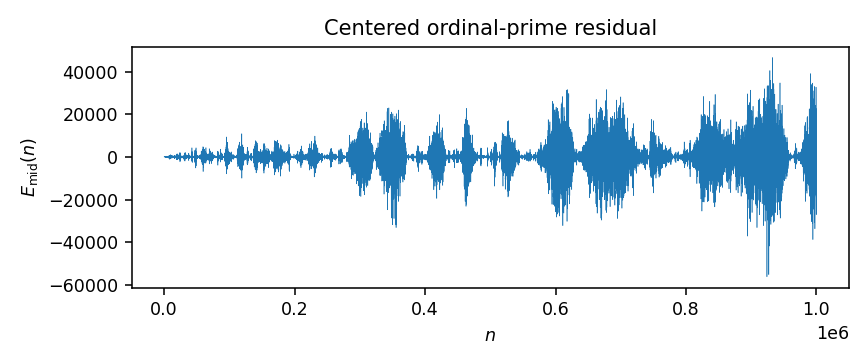
\includegraphics[width=.85\textwidth]{figures/fig1_Emid.png}
\caption[Centered residual up to one million]{$E_{\mathrm{mid}}(n)$ for $n\le10^{6}$.}
\label{fig:residual}
\end{figure}

\subsection{C. The \texorpdfstring{$h^{3/2}$}{h to the three halves} law and its stationarity}
\label{sec:num-scaling}
Put $Z_{3/2}(n):=E_{\mathrm{mid}}(n)/\bigl(|\Mert(n)|^{3/2}\log n\bigr)$.
Conditioning on $h=|\Mert(n)|$ over $n\ge10^{3}$:
\begin{equation}
\label{eq:h-binned-scaling}
\begin{array}{lcccccccc}
\toprule
h\in & [8,12) & [12,19) & [19,31) & [31,51) & [51,84) & [84,138) & [138,225) & [225,400)\\
\midrule
\operatorname{median}|Z_{3/2}| & 0.1426 & 0.1477 & 0.1589 & 0.1589 & 0.1556 & 0.1546 & 0.1507 & 0.1550\\
\text{count} & 36\,451 & 58\,125 & 86\,041 & 127\,696 & 152\,059 & 164\,880 & 231\,986 & 65\,791\\
\bottomrule
\end{array}
\end{equation}
and conditioning on $n$ instead:
\begin{equation}
\label{eq:n-binned-scaling}
\begin{array}{lccc}
\toprule
n\in & \operatorname{RMS}Z_{3/2} & \operatorname{median}|Z_{3/2}| & \text{count}\\
\midrule
{}[1.00,1.58)\times10^{5} & 0.2331 & 0.1549 & 51\,624\\
{}[1.58,2.51)\times10^{5} & 0.2379 & 0.1574 & 82\,660\\
{}[2.51,3.98)\times10^{5} & 0.2340 & 0.1541 & 134\,286\\
{}[3.98,6.31)\times10^{5} & 0.2314 & 0.1530 & 215\,541\\
{}[6.31,10.0)\times10^{5} & 0.2324 & 0.1552 & 359\,873\\
\bottomrule
\end{array}
\end{equation}
Both tables are flat: the normalisation $|\Mert|^{3/2}\log n$ is stable across a
factor of $46$ in $h$ and a factor of $10$ in $n$. This supports, but does not
prove, the hypothesis that $Z_{3/2}$ converges in distribution.

\begin{figure}[htbp]
\centering
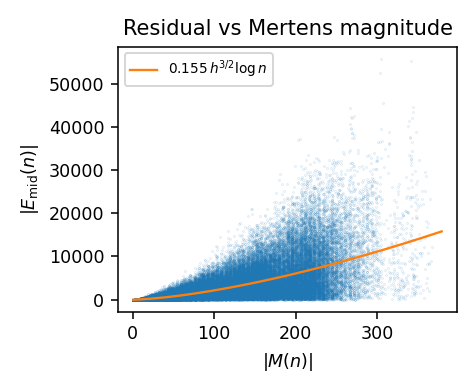
\includegraphics[width=.48\textwidth]{figures/fig2_scaling.png}
\hfill
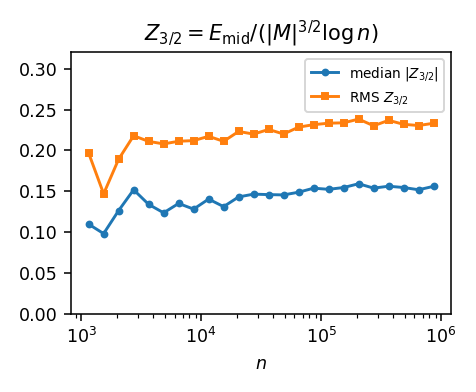
\includegraphics[width=.48\textwidth]{figures/fig3_stationarity.png}
\caption[Residual scaling and stationarity]{Left: $|E_{\mathrm{mid}}|$ against $|\Mert|$ with the envelope
$0.155\,h^{3/2}\log n$. Right: stationarity of $Z_{3/2}$ in $n$.}
\label{fig:scaling-stationarity}
\end{figure}

\subsection{D. Which variance model is right}
\label{sec:num-variance}
Local gap statistics were measured on the prime-index band
$[5\times10^{4},3.05\times10^{5})$, which covers the windows for
$n\in[10^{5},10^{6}]$: mean gap $14.5927$, $\log p=14.6984$ at the band centre,
$\operatorname{Var}(g)=145.93$, hence
\begin{equation}
\label{eq:gap-variance-ratio}
\operatorname{Var}(g)/\log^{2}p=0.6755
\end{equation}
against the value $1$ predicted by a Poisson (Cram\'er) gap model. The gap
autocorrelation is negative at short lag and positive over a long tail:
\begin{equation}
\label{eq:gap-autocorr-table}
\begin{array}{lcccccc}
\toprule
d & 1 & 2 & 3 & 4 & 5 & 6\\
\midrule
\rho(d) & -0.0463 & -0.0225 & -0.0132 & -0.0057 & -0.0069 & -0.0061\\
\bottomrule
\end{array}
\end{equation}
with $\sum_{1\le d\le420}\rho(d)=+0.4646$. The resulting correction factor
decreases steadily,
\begin{equation}
\label{eq:kappa-table}
\begin{array}{lccccccc}
\toprule
h & 5 & 10 & 20 & 40 & 80 & 160 & 320\\
\midrule
\kappa(h) & 1.0206 & 0.9532 & 0.9094 & 0.8514 & 0.7869 & 0.7381 & 0.6871\\
\bottomrule
\end{array}
\end{equation}

Testing both models on the $883\,123$ values of $n$ with $n\ge10^{4}$ and
$h\ge12$:
\begin{equation}
\label{eq:model-comparison-table}
\begin{array}{lcccc}
\toprule
\text{model} & \operatorname{RMS}(E_{\mathrm{mid}})/\operatorname{RMS}(\mathrm{SD}) & \operatorname{RMS}Z & \operatorname{mean}Z & \operatorname{median}|Z| \\
\midrule
\text{independent gaps} & 0.8527 & 0.8963 & -1.88\times10^{-4} & 0.5962\\
\text{covariance-corrected} & 1.0031 & 1.0036 & -2.13\times10^{-4} & 0.6694\\
\bottomrule
\end{array}
\end{equation}
The $15\%$ shortfall of the observed r.m.s.\ relative to the independent-gap
prediction is therefore explained, to within $0.3\%$, by the correlations
between prime gaps; and the corrected model
reproduces the Gaussian value $\operatorname{median}|Z|=0.6745$ to within $0.8\%$
with no free parameter. Within the measured range, this accounts for the scale discrepancy left by the independent model.

\begin{figure}[htbp]
\centering
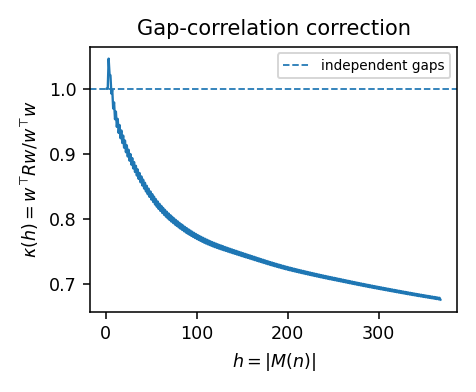
\includegraphics[width=.48\textwidth]{figures/fig4_kappa.png}
\hfill
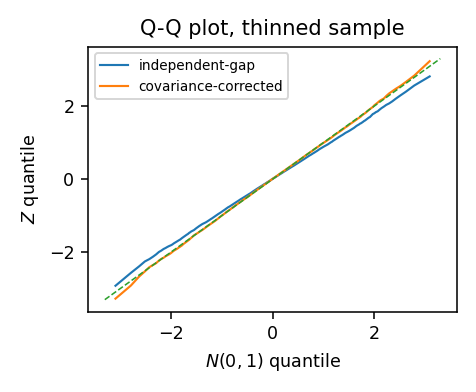
\includegraphics[width=.48\textwidth]{figures/fig5_qq.png}
\caption{Left: the correction factor $\kappa(h)$. Right: quantiles of
$Z=E_{\mathrm{mid}}/\mathrm{SD}$ against the normal, on a thinned sample; the
independent-gap curve is visibly compressed, the corrected one is not.}
\label{fig:kappa-qq}
\end{figure}

\subsection{E. Distribution of the standardised residual}
\label{sec:num-distribution}
With $Z:=E_{\mathrm{mid}}/\operatorname{SD}_{\mathrm{cov}}$, by blocks in $n$
($h\ge12$):
\begin{equation}
\label{eq:z-block-table}
\begin{array}{lcccccc}
\toprule
n\in & \text{count} & \operatorname{mean} & \operatorname{sd} & \text{skew} & \text{exc.\ kurt.} & \operatorname{median}|Z|\\
\midrule
{}[10^{4},10^{5}) & 67\,120 & +0.0043 & 0.9813 & -0.0098 & +0.2556 & 0.6474\\
{}[10^{5},3.16\times10^{5}) & 183\,261 & -0.0000 & 1.0029 & -0.0167 & +0.1559 & 0.6705\\
{}[3.16\times10^{5},10^{6}) & 632\,741 & -0.0008 & 1.0061 & -0.0188 & +0.0957 & 0.6715\\
\bottomrule
\end{array}
\end{equation}
and by blocks in $h$, the excess kurtosis decreases overall, with a small
nonmonotone rise between the fourth and fifth bins,
\begin{equation}
\label{eq:kurtosis-by-h}
\begin{array}{lccccccc}
\toprule
h\in & [12,19) & [19,31) & [31,51) & [51,84) & [84,138) & [138,225) & [225,400)\\
\midrule
\text{exc.\ kurt.} & +0.676 & +0.338 & +0.213 & +0.031 & +0.058 & +0.024 & -0.143\\
\bottomrule
\end{array}
\end{equation}
which is qualitatively consistent with, but does not establish, the behaviour expected if a central limit theorem governs the sum of
Theorem~\ref{thm:gaps} as $h\to\infty$. Quantiles of $Z$ over all $n\ge10^{4}$,
$h\ge12$:
\begin{equation}
\label{eq:quantiles-table}
\begin{array}{lccccccc}
\toprule
\text{level} & 1\% & 5\% & 25\% & 50\% & 75\% & 95\% & 99\%\\
\midrule
\text{observed} & -2.372 & -1.652 & -0.666 & +0.000 & +0.673 & +1.641 & +2.346\\
N(0,1) & -2.326 & -1.645 & -0.674 & 0 & +0.674 & +1.645 & +2.326\\
\bottomrule
\end{array}
\end{equation}

\subsection{F. The points are not independent}
\label{sec:num-dependence}
This is a necessary caveat on the preceding tables. Consecutive $n$ share almost
the same window, so the $883\,123$ values of $Z$ are strongly dependent: the
autocorrelation of $Z$ in $n$ is $+0.979$ at lag $1$, $+0.692$ at lag $10$, and
first falls below $0.05$ at lag $128$. The integrated autocorrelation time is
$\approx51$, giving an effective sample size of about $1.7\times10^{4}$, not
$8.8\times10^{5}$.

Consequently a Kolmogorov--Smirnov test on the full sample is meaningless. On
thinned subsamples:
\begin{equation}
\label{eq:thinning-table}
\begin{array}{lccccc}
\toprule
\text{thinning} & \text{count} & \operatorname{sd} & \text{exc.\ kurt.} & \mathrm{KS} & p\\
\midrule
1 & 883\,123 & 1.0036 & +0.120 & 0.00317 & 3.8\times10^{-8}\\
51 & 17\,317 & 1.0036 & +0.170 & 0.00451 & 0.87\\
128 & 6\,900 & 1.0057 & +0.018 & 0.00775 & 0.80\\
\bottomrule
\end{array}
\end{equation}
On the two thinned samples the reported KS tests do not reject a standard normal
reference law. This is descriptive rather than a proof of normality: thinning reduces
dependence but does not establish independence. The full-sample $p$-value is not
interpreted because the observations are strongly dependent.

\begin{figure}[htbp]
\centering
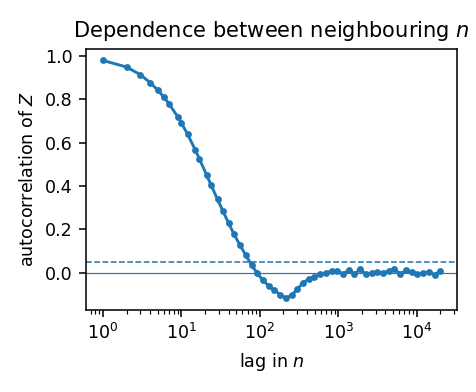
\includegraphics[width=.55\textwidth]{figures/fig6_autocorr.png}
\caption{Autocorrelation of $Z$ in $n$; the effective sample is roughly $50$
times smaller than the nominal one.}
\label{fig:autocorr}
\end{figure}

\subsection{G. Relative size of the residual}
\label{sec:num-relative}
Combining $|E_{\mathrm{mid}}|\approx c\,h^{3/2}\log n$ with $|T|\approx
h\,p^{*}\approx \tfrac{3}{\pi^{2}}h\,n\log n$ predicts
\begin{equation}
\label{eq:relative-residual-prediction}
\begin{aligned}
\frac{|E_{\mathrm{mid}}(n)|}{|T(n)|}
&\approx \frac{c\pi^{2}}{3}\cdot\frac{\sqrt{|\Mert(n)|}}{n},\\
\frac{c\pi^{2}}{3}&=0.510 \qquad (c=0.155).
\end{aligned}
\end{equation}
Measured medians of $\bigl(|E_{\mathrm{mid}}|/|T|\bigr)\,n/\sqrt{|\Mert|}$:
$0.4385,\ 0.4800,\ 0.4995,\ 0.4955$ on
\begin{equation}
\label{eq:relative-residual-ranges}
[10^{3},10^{4}),\quad [10^{4},10^{5}),\quad
[10^{5},3.16\times10^{5}),\quad [3.16\times10^{5},10^{6}).
\end{equation}
This quantitatively explains why the central term reproduces $T$ so accurately.
The measured median satisfies
\begin{equation}
\label{eq:median-relative-residual}
\operatorname{median}_{T(n)\ne0}\frac{|E_{\mathrm{mid}}|}{|T|}=8.9\times10^{-6}.
\end{equation}
If $|\Mert(n)|$ is of size roughly $n^{1/2}$, the relative correction is of
size $n^{-3/4}$.

\subsection{H. Largest excursions}
\label{sec:num-extremes}
The extremes of $E_{\mathrm{mid}}$ on $n\le10^{6}$ occur in tight clusters,
e.g.\ $-5.7654\times10^{4}$ at $n=924\,067$ ($\Mert=-301$) and
$+4.6576\times10^{4}$ at $n=932\,737$ ($\Mert=-269$). These are the $n$ at which
$|\Mert|$ is locally largest, consistent with the $h^{3/2}$ law and carrying no
separate endpoint information.

\subsection{I. The packet envelope}
\label{sec:num-packets}
The visible packets are almost entirely the excursions of $|\Mert(n)|$ passed
through the $h^{3/2}$ variance scale. With a moving RMS window of width $2000$,
the log--log correlation between the measured envelope of $E_{\mathrm{mid}}$
and a moving average of $|\Mert(n)|^{3/2}\log n$ is
\begin{equation}
\label{eq:packet-correlation}
0.9939\qquad(n\ge5\times10^4).
\end{equation}
Replacing the Mertens factor by a trend depending only on $n$ gives correlation
$0.4442$. Figure~\ref{fig:packet-envelope} displays the resulting amplitude
modulation.

\begin{figure}[htbp]
\centering
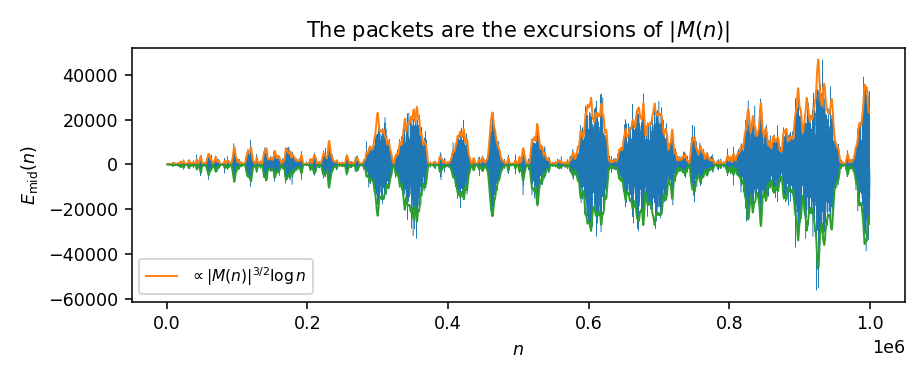
\includegraphics[width=.88\textwidth]{figures/fig7_envelope.png}
\caption{The packet structure of $E_{\mathrm{mid}}$ follows the excursions of
$|M(n)|$. The red curves show a scaled moving average proportional to
$|M(n)|^{3/2}\log n$.}\label{fig:packet-envelope}
\end{figure}

\subsection{J. Spectrum on the logarithmic coordinate: a classical check}
\label{sec:num-spectrum}
Put $u=\log x$ and, for integer samples $x=n$, consider
\begin{equation}
\label{eq:log-coordinate-signal}
X(u):=e^{-u/2}\Mert(\lfloor e^u\rfloor).
\end{equation}
The classical Perron/explicit-formula treatment of the Mertens function \cite{Titchmarsh1986}, after
truncation and contour displacement and under the usual hypotheses on the zeros, has
residue contributions of the form
\begin{equation}
\label{eq:explicit-formula-mode}
\frac{x^{\rho}}{\rho\zeta'(\rho)}.
\end{equation}
For a simple zero $\rho=\beta+i\gamma$, the corresponding contribution after
$x=e^u$ and multiplication by $e^{-u/2}$ is proportional to
$e^{(\beta-1/2)u}e^{i\gamma u}$. Under RH this becomes a pure mode
$e^{i\gamma u}$. Consequently, within that classical explicit-formula framework,
the appearance of power at
frequencies $\gamma_k$ in $X(u)$ is the expected explicit-formula behaviour,
not a new law of the transform. Historical numerical uses of zeta zeros to reconstruct
prime-counting structure include \cite{RieselGohl1970}.

The numerical spectrum over $10^3\le n\le10^6$ (after the interpolation and
windowing used by the supplied script) shows peaks near the first zeta
ordinates, while a random-sign surrogate with the same squarefree support does
not show the same visual alignment. The original peak-to-nearest-zero summary
(mean distances $0.263$ for the true sequence and $1.738$ for one surrogate)
has a selection bias because peaks were selected before matching them to the
zeros. It is retained only as a diagnostic and not used as evidence. The proper
fixed-frequency question is the power evaluated at preassigned $\gamma_k$, or a
regression on the preassigned modes.

More fundamentally, the finite logarithmic window itself imposes the resolution
\begin{equation}
\label{eq:frequency-resolution}
\Delta\omega\simeq\frac{2\pi}{u_{\max}-u_{\min}}
 =\frac{2\pi}{\log(10^6/10^3)}\simeq0.91.
\end{equation}
Peak offsets of a few tenths are therefore below the resolving power of this finite
window and carry no precision information about the known $\gamma_k$. Doubling the
frequency resolution requires doubling the range in $u$, hence squaring the
range in $n$; reaching resolution $10^{-3}$ would require a logarithmic span of
order $2\pi\times10^3$, far outside this computation.

\begin{figure}[htbp]
\centering
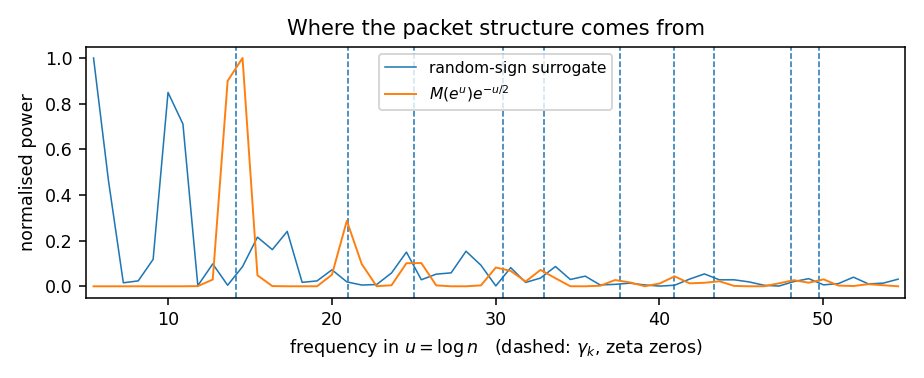
\includegraphics[width=.88\textwidth]{figures/fig8_spectrum.png}
\caption{Power spectrum of $M(e^u)e^{-u/2}$ on $u=\log n$. Dashed lines are the
first zeta ordinates. This is an illustration of the classical explicit-formula
modes; the peak-matching statistic is not used inferentially because of
selection bias and finite-window resolution.}\label{fig:spectrum}
\end{figure}

\subsection{K. Prime-counting variance comparison}
\label{sec:num-prime-variance}
Proposition~\ref{prop:pi-integral} puts the residual on the prime-counting side.
At prime scale $X\simeq4.3\times10^6$, the supplied experiment compares the
measured variance of short-interval prime counts with an $H\log(X/H)$ reference
scale motivated by Montgomery and Soundararajan for weighted prime counts
$\psi(x+H)-\psi(x)$, and with a Poisson/Cram\'er-type $H\log X$ reference.
This is only a scale comparison. It is not a direct application of the
Montgomery--Soundararajan statement \cite{MontgomerySoundararajan2004} to the
unweighted count $\pi(x+H)-\pi(x)$. The Poisson comparison is in the spirit of
Cram\'er's model \cite{Cramer1936}. The reported ratios are
\begin{equation}
\label{eq:short-interval-variance-table}
\begin{array}{lrrrr}
\toprule
H & 200 & 1000 & 5000 & 20000\\
\midrule
\operatorname{Var}_{\rm meas}/\operatorname{Var}_{\rm MS}
 &1.116&1.202&1.310&1.622\\
\operatorname{Var}_{\rm meas}/\operatorname{Var}_{\rm Cramer}
 &0.552&0.468&0.372&0.314\\
\bottomrule
\end{array}
\end{equation}
The decreasing ratio to the Cram\'er scale is the expected qualitative signature
of an $H\log(X/H)$ variance rather than $H\log X$. The excess over the leading
MS term is not interpreted as a new statistic: at $H=2\times10^4$ the displayed
leading logarithmic factor is only about $2.96$, versus $\log X\simeq15.3$, so
lower-order terms are not negligible in this preasymptotic range.

\subsection{L. Cross-coupling test}
\label{sec:coupling}
The only numerical loophole left inside $E_{\mathrm{mid}}$ is weaker than new
endpoint information. The gap factor in Theorem~\ref{thm:gaps} is controlled by
prime statistics, while the window length is $h=|M(n)|$. One can ask whether
the standardised fluctuation
\begin{equation}
\label{eq:standardized-residual}
Z(n)=\frac{E_{\mathrm{mid}}(n)}{\operatorname{SD}_{\mathrm{cov}}(n)},
\qquad h=|M(n)|\ge12,
\end{equation}
is coupled to the sign or to a zeta phase of $M$. The supplied follow-up tests
reported
\begin{equation}
\label{eq:coupling-table}
\begin{array}{lc}
\toprule
\text{test} & \text{value}\\
\midrule
\operatorname{corr}(Z,\operatorname{sgn}M) & +0.00058\\
\operatorname{corr}(Z,M/\sqrt n) & +0.00110\\
\operatorname{corr}(Z,\cos(\gamma_1\log n)) & -0.00119\\
\operatorname{corr}(Z,\sin(\gamma_1\log n)) & +0.00173\\
\overline Z\,|_{M>0}-\overline Z\,|_{M<0} & +0.00027\quad(0.08\sigma\ \text{effective})\\
\bottomrule
\end{array}
\end{equation}
and an eight-bin phase test gave dispersion of the bin means $0.00070$, compared
with a typical standard error $0.00499$.

These are null results only at the tested resolution. With effective sample
$n_{\rm eff}\simeq17\,316$, the nominal standard error of a small correlation is
$1/\sqrt{n_{\rm eff}}\simeq0.0076$, so the experiment excludes only linear
couplings of order $|r|\gtrsim0.015$. Weaker effects, nonlinear dependence,
untested functions of the phase, or effects emerging only at much larger $n$
remain outside the sensitivity of this computation. The result therefore does
\emph{not} prove decoupling; it says that no coupling was detected in this small
specified family.

\section{Status of the claims}
\label{sec:status}

To keep the register unambiguous:
\begin{itemize}[leftmargin=1.6em]
\item \emph{Proved}: Lemmas~\ref{lem:counters}, \ref{lem:parity}, \ref{lem:w2};
Propositions~\ref{prop:closed}, \ref{prop:block}, \ref{prop:scale},
\ref{prop:info}, \ref{prop:offset}, \ref{prop:pairing-endpoints},
\ref{prop:pairing-rh}, \ref{prop:d-parity-cancellation},
\ref{prop:coercivity-evenisation}, \ref{prop:D-real-axis-counterexample},
\ref{prop:survival-kernel-collapse}, \ref{prop:active-lifetime-first-moment},
and \ref{prop:multicut-convexity-collapse}, \ref{prop:phi-fibres},
\ref{prop:phi-escape-rate}, \ref{prop:ss-parity}, and
\ref{prop:length-two-collision}, \ref{prop:crossing-values}, and
\ref{prop:nonprime-controls}; Corollaries~\ref{cor:bounds} and
\ref{cor:fixed-window-variance}; Theorems~\ref{thm:RH}, \ref{thm:gaps},
\ref{thm:quadratic-pairing}, \ref{thm:sf-log-chowla-two},
\ref{thm:universal-coding}, \ref{thm:sqrt-recovery}, and
\ref{thm:phi-dynamics}, \ref{thm:level-return},
\ref{thm:negative-excursion-energy}, and
\ref{thm:prime-ordinal-amplification}; the exact
identities \eqref{eq:H3-increment}, \eqref{eq:P-autocorrelation-hpoint},
\eqref{eq:weighted-lifetime-active-block}, and
\eqref{eq:character-block-energy}; and the mean-square criterion
\eqref{eq:mean-square-rh-criterion}.
\item \emph{Measured}, over $10^{4}\le n\le10^{6}$ with effective sample
$\approx1.7\times10^{4}$ where relevant: the law
$|E_{\mathrm{mid}}|\approx0.155\,|\Mert|^{3/2}\log n$; the failure of the
independent-gap model, which overpredicts the observed r.m.s.\ by the reciprocal
of the ratio $0.853$, and its repair by the measured gap covariance; approximate normality of the standardised residual; the
$0.9939$ packet-envelope correlation; the exact finite $\kappa$--$\rho$ transform (regenerated to double-precision
roundoff) and the reported finite-dimensional recovery of the first lags of $\rho$
from $\kappa$; the short-interval variance ratios; the
null cross-coupling tests of Section~\ref{sec:coupling}; and the Version 6
quadratic-energy and center-displacement measurements in
Experiments~\ref{exp:v6-quadratic-controls} and~\ref{exp:v6-center-scale};
the signed third-moment measurement in Experiment~\ref{exp:v7-third-moment},
which is explicitly recorded with drift and without an asymptotic exponent claim;
and the conditioned active-lifetime comparison in
Experiment~\ref{exp:active-lifetime-shape}.
The finite level-collision, excursion, and occupancy counts in
Experiment~\ref{exp:v11-entropy-controls} are also measured diagnostics; the
identities checked there are proved separately and do not depend on those
counts.
\item \emph{Classical interpretation, not novelty}: the frequencies $\gamma_k$
in the $u=\log n$ spectrum of $M(e^u)e^{-u/2}$ are the modes supplied by the
explicit formula. The displayed peak matching is diagnostic only and has
frequency resolution about $0.91$.
\item \emph{Conjectural}: that $Z_{3/2}$ converges in distribution; that the
limit is Gaussian; that a central limit theorem holds for the antisymmetric
weighted gap sum of Theorem~\ref{thm:gaps}; that the observed numerical
absence of cross-coupling persists asymptotically; or that
$\mathcal D_2/(2\mathcal M_2)\to1$. None follows from the present numerics.
\item \emph{Closed or classified negative routes}: the quadratic orthogonal split
\eqref{eq:parallelogram-energy} is pairing-insensitive, and the proposed
uniform contraction $\mathcal E_2\ge\delta\mathcal D_2$ is not supported; the
reported ratio decreases strongly with scale.  The root-of-unity prefix filter
reduces exactly to higher-order consecutive correlations by
\eqref{eq:P-autocorrelation-hpoint}; universal coercivity can be evenised by
Proposition~\ref{prop:coercivity-evenisation}; the real-axis generating
function is not uniformly coercive by Proposition~\ref{prop:D-real-axis-counterexample};
and the two-cut survival kernel collapses to endpoint heights by
Proposition~\ref{prop:survival-kernel-collapse}.  Question~\ref{q:multimodulus-coercivity}
remains an open mechanism, not a claimed consequence of the large sieve.
\end{itemize}


\section{Ordinal pairing and the quadratic route}
\label{sec:ordinal-pairing}

This section records a second representation that arises directly from the two
sign-specific ordinal counters.  Unlike the prime-gap residual, the construction
below uses only the order in which the nonzero values of $\mu$ occur.  It is useful
because it gives an exact transport picture of the squarefree-time Mertens walk;
it does \emph{not} create an independent bound on that walk.

Let
\begin{equation}
\label{eq:squarefree-order}
s_1<s_2<\cdots
\end{equation}
be the squarefree positive integers, and define the squarefree-time sign sequence
and its partial sums by
\begin{equation}
\label{eq:squarefree-walk}
\varepsilon_q:=\mu(s_q)\in\{-1,+1\},
\qquad
R(q):=\sum_{r\le q}\varepsilon_r=M(s_q).
\end{equation}
Let $\alpha_j$ be the squarefree ordinal of the $j$-th occurrence of $+1$, and
$\beta_j$ the squarefree ordinal of the $j$-th occurrence of $-1$.  Thus
\begin{equation}
\label{eq:pairing-definitions}
\varepsilon_{\alpha_j}=+1,
\qquad
\varepsilon_{\beta_j}=-1,
\qquad
d_j:=\beta_j-\alpha_j,
\qquad
c_j:=\frac{\alpha_j+\beta_j}{2},
\qquad
e_j:=c_j-2j.
\end{equation}
The corresponding separation in the original integer coordinate is
\begin{equation}
\label{eq:integer-pairing-displacement}
\Delta_j:=s_{\beta_j}-s_{\alpha_j}.
\end{equation}
The sign of $d_j$ records which member of the ordinal pair occurs first.

\begin{proposition}[Exact endpoint identities]
\label{prop:pairing-endpoints}
For every $j\ge1$,
\begin{align}
\alpha_j+R(\alpha_j)&=2j,
\label{eq:alpha-endpoint}\\[2mm]
\beta_j-R(\beta_j)&=2j,
\label{eq:beta-endpoint}
\end{align}
and hence
\begin{align}
d_j&=R(\alpha_j)+R(\beta_j),
\label{eq:d-endpoint-sum}\\
2e_j&=R(\beta_j)-R(\alpha_j).
\label{eq:e-endpoint-difference}
\end{align}
Moreover,
\begin{equation}
\label{eq:e-lipschitz}
|2e_j|\le |d_j|.
\end{equation}
\end{proposition}

\begin{proof}
At $q=\alpha_j$, the number of positive signs is $j$, so
$j=(\alpha_j+R(\alpha_j))/2$; similarly
$j=(\beta_j-R(\beta_j))/2$.  Adding and subtracting these two endpoint
relations gives \eqref{eq:d-endpoint-sum} and
\eqref{eq:e-endpoint-difference}.  Finally, $R$ changes by exactly $\pm1$ at
each squarefree-time step, hence it is $1$-Lipschitz on the integer variable
$q$ and
\begin{equation}
\label{eq:R-lipschitz-pair}
|R(\beta_j)-R(\alpha_j)|\le |\beta_j-\alpha_j|.
\end{equation}
Together with \eqref{eq:e-endpoint-difference}, this is
\eqref{eq:e-lipschitz}.
\end{proof}

\begin{proposition}[Pairing criterion for RH]
\label{prop:pairing-rh}
The following are equivalent:
\begin{enumerate}[label=(\alph*)]
\item the Riemann hypothesis;
\item for every $\varepsilon>0$,
\begin{equation}
\label{eq:d-rh-criterion}
d_j=O_\varepsilon\!\left(j^{1/2+\varepsilon}\right);
\end{equation}
\item for every $\varepsilon>0$,
\begin{equation}
\label{eq:Delta-rh-criterion}
\Delta_j=O_\varepsilon\!\left(j^{1/2+\varepsilon}\right).
\end{equation}
\end{enumerate}
\end{proposition}

\begin{proof}
Under RH, the classical Littlewood criterion gives
$M(x)=O_\varepsilon(x^{1/2+\varepsilon})$; since $s_q\asymp q$, equation
\eqref{eq:d-endpoint-sum} gives \eqref{eq:d-rh-criterion}.
Conversely, fix $q$ and write $h=|R(q)|$.  If $R(q)>0$, exactly $h$ ordinal
pairs are open across the cut after $q$, namely the pairs whose positive member
has occurred and whose negative member has not.  For
$j=N_-(q)+r$, $1\le r\le h$, there are at least $h-r$ subsequent positive
members before the cut and at least $r$ negative members still required after
the cut.  Therefore
\begin{equation}
\label{eq:open-pair-lower-bound}
|d_j|\ge h.
\end{equation}
The case $R(q)<0$ is identical with the signs interchanged.  Since every such
open index satisfies $j\le q$, \eqref{eq:d-rh-criterion} yields
$|R(q)|=O_\varepsilon(q^{1/2+\varepsilon})$.  As $R(q)=M(s_q)$ and $s_q\asymp q$,
this gives the Littlewood criterion and hence RH.

For the original integer displacement, first note that $\Mert(x)=o(x)$ (PNT)
gives $R(q)=o(q)$, hence $N_\pm(q)=(q\pm R(q))/2=q/2+o(q)$; inverting the
counters gives $\alpha_j,\beta_j=(2+o(1))j$.  With this, the standard squarefree
counting estimate \cite{Apostol1976}
\begin{equation}
\label{eq:squarefree-inverse}
s_q=\frac{\pi^2}{6}q+O(\sqrt q)
\end{equation}
gives $\Delta_j=\tfrac{\pi^2}{6}d_j+O(\sqrt j)$ and hence shows that
\eqref{eq:d-rh-criterion} implies \eqref{eq:Delta-rh-criterion}.  Conversely, monotonicity of $s_q$ gives
$|d_j|\le|\Delta_j|$, so \eqref{eq:Delta-rh-criterion} implies
\eqref{eq:d-rh-criterion}.
\end{proof}

The point of Proposition~\ref{prop:pairing-rh} is representational rather than
inferential: testing a $j^{1/2}$ scale numerically is only a compatibility test
for RH.  It cannot establish the required uniform bound.

\subsection{Quadratic energy on a balanced prefix}
\label{subsec:quadratic-energy}

Fix a squarefree-time prefix $Q$ satisfying
\begin{equation}
\label{eq:balanced-prefix}
R(Q)=0,
\qquad
J:=Q/2.
\end{equation}
Then the first $Q$ squarefree signs contain exactly $J$ positive and $J$
negative values, so $\{\alpha_1,\ldots,\alpha_J\}$ and
$\{\beta_1,\ldots,\beta_J\}$ partition $\{1,\ldots,Q\}$.  Define
\begin{equation}
\label{eq:quadratic-energies}
\mathcal M_2(Q):=\sum_{q\le Q}R(q)^2,
\qquad
\mathcal D_2(J):=\sum_{j\le J}d_j^2,
\qquad
\mathcal E_2(J):=4\sum_{j\le J}e_j^2.
\end{equation}

\begin{theorem}[Exact quadratic identity and comparison]
\label{thm:quadratic-pairing}
On every balanced prefix \eqref{eq:balanced-prefix},
\begin{equation}
\label{eq:endpoint-energy-partition}
\sum_{j\le J}\bigl(R(\alpha_j)^2+R(\beta_j)^2\bigr)
=\mathcal M_2(Q),
\end{equation}
\begin{equation}
\label{eq:parallelogram-energy}
\boxed{\;\mathcal D_2(J)+\mathcal E_2(J)=2\mathcal M_2(Q)\;},
\end{equation}
and
\begin{equation}
\label{eq:quadratic-comparison}
\boxed{\;\mathcal M_2(Q)\le\mathcal D_2(J)\le2\mathcal M_2(Q)\;}.
\end{equation}
\end{theorem}

\begin{proof}
Equation \eqref{eq:endpoint-energy-partition} follows because every
$q\in\{1,\ldots,Q\}$ occurs exactly once as an $\alpha_j$ or as a $\beta_j$.
For each ordinal pair, equations \eqref{eq:d-endpoint-sum} and
\eqref{eq:e-endpoint-difference} give the parallelogram identity
\begin{equation}
\label{eq:pairwise-parallelogram}
d_j^2+4e_j^2
=2R(\alpha_j)^2+2R(\beta_j)^2.
\end{equation}
Summing \eqref{eq:pairwise-parallelogram} and using
\eqref{eq:endpoint-energy-partition} proves
\eqref{eq:parallelogram-energy}.  The upper bound in
\eqref{eq:quadratic-comparison} follows from $\mathcal E_2\ge0$.  The
Lipschitz inequality \eqref{eq:e-lipschitz} gives
$\mathcal E_2\le\mathcal D_2$; substituting this into
\eqref{eq:parallelogram-energy} gives the lower bound.
\end{proof}

\begin{remark}[Why the orthogonal decomposition is not a transport gain]
\label{rem:pairing-insensitive}
Let $x_j:=R(\alpha_j)$ and $y_j:=R(\beta_j)$.  For any permutation $\pi$ of
$\{1,\ldots,J\}$,
\begin{equation}
\label{eq:permutation-parallelogram}
\sum_{j\le J}\Bigl((x_j+y_{\pi(j)})^2+(y_{\pi(j)}-x_j)^2\Bigr)
=2\sum_{j\le J}x_j^2+2\sum_{j\le J}y_j^2
=2\mathcal M_2(Q).
\end{equation}
Thus the $45^\circ$ energy split itself is independent of how the two endpoint
sets are paired.  The ordinal matching is special only because for $\pi(j)=j$
the two rotated coordinates are exactly $d_j$ and $2e_j$.  Consequently
\eqref{eq:parallelogram-energy} cannot by itself generate an iterative or
multiscale gain.
\end{remark}

\subsection{Mean-square criterion and closure of the quadratic route}
\label{subsec:quadratic-closure}

The comparison \eqref{eq:quadratic-comparison} shows that, on balanced
prefixes, the quadratic transport energy and the squarefree-time mean square of
Mertens differ by at most an absolute factor two.  Independently of the
pairing, the following mean-square criterion is equivalent to RH:
\begin{equation}
\label{eq:mean-square-rh-criterion}
\mathrm{RH}
\quad\Longleftrightarrow\quad
\mathcal M_2(Q)=O_\varepsilon\!\left(Q^{2+\varepsilon}\right)
\quad\text{for every }\varepsilon>0.
\end{equation}
Indeed RH implies the bound termwise. Conversely, extend $R$ as a step function
on the nonnegative reals. If \eqref{eq:mean-square-rh-criterion} holds,
Cauchy--Schwarz on dyadic blocks shows that the Mellin integral
\begin{equation}
\label{eq:squarefree-sign-dirichlet}
F(s):=s\int_1^\infty R(t)t^{-s-1}\,dt
\end{equation}
converges absolutely and is holomorphic for $\Re s>1/2$; for $\Re s>1$ it equals
$\sum_{q\ge1}\varepsilon_q q^{-s}$ by summation by parts. This first constructs
analytic continuation, rather than assuming ordinary series convergence in
the larger half-plane. Since \eqref{eq:squarefree-inverse} gives, uniformly on compact
subsets of that half-plane,
\begin{equation}
\label{eq:squarefree-weight-comparison}
s_q^{-s}=\left(\frac{\pi^2}{6}q\right)^{-s}
+O_s\!\left(q^{-\Re s-1/2}\right),
\end{equation}
the difference between
$\sum_q\varepsilon_q s_q^{-s}=1/\zeta(s)$ and
$(\pi^2/6)^{-s}F(s)$ is absolutely convergent there.  Hence $1/\zeta(s)$ has a
holomorphic continuation to $\Re s>1/2$, which excludes zeros of $\zeta$ in
that half-plane; the functional equation then gives RH.

Thus a proof of
\begin{equation}
\label{eq:D2-target}
\mathcal D_2(J)=O_\varepsilon\!\left(J^{2+\varepsilon}\right)
\end{equation}
would be useful only if it were obtained by an argument genuinely easier than,
or independent of, the corresponding mean-square estimate for $R$.  The exact
comparison \eqref{eq:quadratic-comparison} shows that the ordinal pairing does
not soften the quadratic problem merely by changing coordinates.

The mean-square behaviour of the Mertens function and its limiting
distribution under additional hypotheses on negative moments of
$\zeta'(\rho)$ are classical subjects; see, for example, Ng
\cite{Ng2004}.  In particular, one should not identify a finite quadratic fit
with a new zeta-statistical law.

\begin{experiment}[Regenerated controls for the quadratic decomposition]
\label{exp:v6-quadratic-controls}
The following controls were regenerated in Python from the Version 9 data
arrays by the supplied audit scripts.  On the
balanced prefix
\begin{equation}
\label{eq:v6-balanced-range}
Q=488868,
\qquad
J=244434,
\end{equation}
the exact identities
\eqref{eq:endpoint-energy-partition}, \eqref{eq:d-endpoint-sum},
\eqref{eq:e-endpoint-difference}, \eqref{eq:parallelogram-energy}, and
\eqref{eq:quadratic-comparison} were checked without discrepancy.  The regenerated
energies are
\begin{equation}
\label{eq:v6-energy-values}
\mathcal D_2=10646184520,
\qquad
\mathcal E_2=36823324,
\qquad
2\mathcal M_2=10683007844.
\end{equation}
The resulting fractions are
\begin{equation}
\label{eq:v6-energy-fractions}
\frac{\mathcal D_2}{2\mathcal M_2}=0.99655,
\qquad
\frac{\mathcal E_2}{2\mathcal M_2}=0.00345.
\end{equation}
As a structural control, the total parallelogram energy was unchanged when the
endpoint heights were paired ordinally, randomly, or in reverse order, exactly
as predicted by Remark~\ref{rem:pairing-insensitive}.

On balanced prefixes with $J\ge8000$ through $J=244434$, regenerated log--log
fits gave
\begin{equation}
\label{eq:v6-power-fits}
\mathcal D_2\approx C_{\mathcal D}J^{2.0163},
\qquad
\mathcal E_2\approx C_{\mathcal E}J^{1.4641},
\qquad
\mathcal M_2\approx C_{\mathcal M}J^{2.0120},
\end{equation}
Over the same selected range the ratio $\mathcal E_2/\mathcal D_2$ decreased
from $0.01909$ to $0.00346$.
These finite-range measurements are consistent with
$\mathcal D_2/(2\mathcal M_2)\to1$, but do not prove that asymptotic statement.
They do not support, on the measured range and trend, the proposed
uniform lower comparison
\begin{equation}
\label{eq:false-contraction}
\mathcal E_2\ge\delta\mathcal D_2
\qquad(\delta>0\ \text{fixed}),
\end{equation}
as a plausible multiscale mechanism.  A finite sample whose smallest observed
ratio is positive cannot refute the existence of some $\delta>0$: it excludes
only constants larger than $\min_J\mathcal E_2(J)/\mathcal D_2(J)$ on the
measured range.  A refutation would require proving that the infimum of the
ratio is zero, exhibiting an admissible sequence along which it tends to zero,
or finding a prefix with $\mathcal E_2=0<\mathcal D_2$.
\end{experiment}

\begin{experiment}[Scale of the center displacement]
\label{exp:v6-center-scale}
Equation \eqref{eq:e-endpoint-difference} shows exactly that $2e_j$ is the
increment of the same squarefree-time Mertens walk across the ordinal-pair
window, whose length is $|d_j|$.  The regenerated conditional RMS values were
\begin{center}
\begin{tabular}{@{}ccccc@{}}
\toprule
$|d|$ bin & $15$--$23$ & $56$--$87$ & $136$--$211$ & $328$--$510$\\
\midrule
$\operatorname{RMS}(2e)/|d|^{1/2}$
& $1.006$ & $1.023$ & $0.979$ & $0.980$\\
$\operatorname{RMS}(2e)/|d|$
& $0.231$ & $0.121$ & $0.075$ & $0.049$\\
\bottomrule
\end{tabular}
\end{center}
A separate log-binned median fit gave exponents $0.2400$ for $|e_j|$ and
$0.4689$ for $|d_j|$.  These finite-range fits are consistent with
the heuristic relation
\begin{equation}
\label{eq:e-sqrt-d-heuristic}
|e_j|\ \text{of typical size}\ |d_j|^{1/2},
\end{equation}
not with $e_j$ providing a second matching energy at the same scale.  No
independence is asserted: both quantities are increments of the same walk.
\end{experiment}

\begin{remark}[Negative result: no quadratic recursion]
\label{rem:no-quadratic-recursion}
Two proposed mechanisms are therefore closed.  First,
\eqref{eq:parallelogram-energy} is a pairing-insensitive parallelogram identity,
so its orthogonal form contains no recursive transport information.  Second,
the candidate lower bound \eqref{eq:false-contraction} is not supported by the
regenerated energy split, with the logical reservation recorded in
Experiment~\ref{exp:v6-quadratic-controls}, while $e_j$ has the same number of terms as $d_j$ and
is merely the half-increment \eqref{eq:e-endpoint-difference} of the original
walk.  The quadratic ordinal representation remains mathematically exact, but
at this level it is a re-expression of the classical Mertens mean-square
problem rather than a new source of leverage.
\end{remark}



\section{Local ordinal correlations beyond quadratic energy}
\label{sec:ordinal-local}

The quadratic comparison in Section~\ref{sec:ordinal-pairing} closes the route
through norms of the displacement sequence, but it does not exhaust the ordinal
pairing.  Local statistics depend on the order of the squarefree signs rather
than only on the multiset of heights $\{R(q)\}$.  This section isolates the
first unconditional result of that type.

For fixed $h\ge1$ define the squarefree-ordinal two-point correlation
\begin{equation}
\label{eq:sf-two-point-correlation}
C_h^{\mathrm{sf}}(Q)
:=\frac{1}{\log Q}\sum_{q\le Q}
\frac{\varepsilon_q\varepsilon_{q+h}}{q}.
\end{equation}
The averaging in \eqref{eq:sf-two-point-correlation} is logarithmic.  The
corresponding natural average is not claimed here.  Results of
Matom\"aki--Radziwi\l\l on cancellation and sign changes of multiplicative
functions in short intervals concern the natural integer clock
\cite{MatomakiRadziwill2016}; they do not directly imply the squarefree-ordinal
statement below, whose proof instead returns to fixed affine forms and uses
Tao's logarithmically averaged two-point theorem.

\begin{theorem}[Logarithmic two-point Chowla in squarefree ordinal time]
\label{thm:sf-log-chowla-two}
For every fixed integer $h\ge1$,
\begin{equation}
\label{eq:sf-log-chowla-two}
\boxed{\;
\sum_{q\le Q}\frac{\mu(s_q)\mu(s_{q+h})}{q}=o(\log Q)
\;}
\qquad(Q\to\infty).
\end{equation}
\end{theorem}

\begin{proof}
Write
\begin{equation}
\label{eq:squarefree-density-constant}
c:=\frac{\pi^2}{6}.
\end{equation}
The squarefree inverse estimate \eqref{eq:squarefree-inverse} gives
\begin{equation}
\label{eq:ordinal-natural-weight-change}
\frac1q=\frac{c}{s_q}+O(q^{-3/2}),
\end{equation}
so replacing $1/q$ by $c/s_q$ changes the sum in
\eqref{eq:sf-log-chowla-two} by $O(1)$.

For each $q$ put
\begin{equation}
\label{eq:physical-gap-h}
r_q:=s_{q+h}-s_q.
\end{equation}
If $n=s_q$ and $r=r_q$, then $n$ and $n+r$ are squarefree and there are
exactly $h-1$ squarefree integers strictly between them.  Since the factor
$\mu(n)\mu(n+r)$ already vanishes unless both endpoints are squarefree, define
\begin{equation}
\label{eq:boolean-squarefree-gap}
W_{h,r}(n)
:=\mathbf 1\!\left\{
\sum_{a=1}^{r-1}\mu(n+a)^2=h-1
\right\}.
\end{equation}
After the change of clock, the contribution with fixed physical separation
$r$ is therefore
\begin{equation}
\label{eq:fixed-r-weighted-correlation}
\sum_{n\le X}
\frac{\mu(n)\mu(n+r)}{n}W_{h,r}(n),
\end{equation}
up to endpoint terms which are $O(1)$ after logarithmic weighting.

Fix $D\ge2$ and introduce the periodic squarefree approximation
\begin{equation}
\label{eq:nu-D-definition}
\nu_D(m):=
\mathbf 1_{\{p^2\nmid m\ \text{for every prime }p\le D\}}.
\end{equation}
It differs from $\mu(m)^2$ only when $p^2\mid m$ for some prime $p>D$.
Consequently
\begin{equation}
\label{eq:nu-D-log-error}
\sum_{m\le X}\frac{|\nu_D(m)-\mu(m)^2|}{m}
\ll \frac{\log X}{D}+O(1).
\end{equation}
For fixed $h$ and $r$, replacing every interior $\mu(n+a)^2$ in
\eqref{eq:boolean-squarefree-gap} by $\nu_D(n+a)$ therefore incurs
\begin{equation}
\label{eq:W-D-log-error}
\sum_{n\le X}\frac{|W_{h,r}(n)-W_{h,r}^{(D)}(n)|}{n}
\ll_r \frac{\log X}{D}+O_r(1),
\end{equation}
where
\begin{equation}
\label{eq:W-D-definition}
W_{h,r}^{(D)}(n)
:=\mathbf 1\!\left\{
\sum_{a=1}^{r-1}\nu_D(n+a)=h-1
\right\}.
\end{equation}

Set
\begin{equation}
\label{eq:MD-definition}
M_D:=\prod_{p\le D}p^2.
\end{equation}
The function $W_{h,r}^{(D)}$ is periodic modulo $M_D$.  Hence there is a
fixed set of residue classes $\mathcal A_{h,r,D}\subseteq\mathbf Z/M_D\mathbf Z$
such that
\begin{equation}
\label{eq:WD-residue-expansion}
W_{h,r}^{(D)}(n)=
\sum_{a\in\mathcal A_{h,r,D}}
\mathbf 1_{n\equiv a\pmod{M_D}}.
\end{equation}
For one such residue class, write $n=M_Dm+a$.  The two M\"obius factors become
\begin{equation}
\label{eq:two-affine-forms}
\mu(M_Dm+a)\mu(M_Dm+a+r).
\end{equation}
The two affine forms have determinant
\begin{equation}
\label{eq:affine-form-determinant}
M_D(a+r)-M_Da=M_Dr\ne0.
\end{equation}
Tao's logarithmically averaged two-point Elliott theorem applies to fixed
nondegenerate affine forms and, in particular, to the M\"obius function
\cite{Tao2016}.  Thus, with $D,r,a$ fixed,
\begin{equation}
\label{eq:Tao-fixed-class}
\sum_{m\le X}
\frac{\mu(M_Dm+a)\mu(M_Dm+a+r)}{m}
=o(\log X).
\end{equation}
Moreover
\begin{equation}
\label{eq:weight-affine-adjustment}
\frac1{M_Dm+a}=\frac1{M_Dm}+O_{D,a}(m^{-2}),
\end{equation}
so the same conclusion holds with the original weight $1/n$.  Because
$D$ and $r$ are fixed, only finitely many residue classes occur; no uniformity
in a growing modulus is required.  Combining this with
\eqref{eq:W-D-log-error}, letting $X\to\infty$ first and then $D\to\infty$,
gives
\begin{equation}
\label{eq:fixed-r-vanishing}
\sum_{n\le X}
\frac{\mu(n)\mu(n+r)}{n}W_{h,r}(n)=o(\log X)
\end{equation}
for every fixed $h$ and $r$.

It remains to remove the truncation in $r$.  The first moment of $r_q$ is
controlled exactly by telescoping:
\begin{align}
\sum_{q\le Q}(s_{q+h}-s_q)
&=\sum_{i=1}^{h}s_{Q+i}-\sum_{i=1}^{h}s_i,
\label{eq:r-gap-telescope}\\
\frac1Q\sum_{q\le Q}r_q
&\longrightarrow ch.
\label{eq:r-gap-first-moment}
\end{align}
Therefore, for
\begin{equation}
\label{eq:r-tail-count}
A_R(Q):=\#\{q\le Q:r_q>R\},
\end{equation}
Markov's inequality gives
\begin{equation}
\label{eq:r-tail-Markov}
A_R(Q)\le\left(\frac{ch}{R}+o(1)\right)Q.
\end{equation}
Partial summation yields
\begin{equation}
\label{eq:r-tail-logarithmic}
\limsup_{Q\to\infty}\frac1{\log Q}
\sum_{\substack{q\le Q\\r_q>R}}\frac1q
\le\frac{ch}{R}.
\end{equation}
For fixed $R$, the finitely many contributions $h\le r\le R$ vanish after
normalisation by $\log Q$ by \eqref{eq:fixed-r-vanishing}; then
\eqref{eq:r-tail-logarithmic} tends to zero as $R\to\infty$.  This proves
\eqref{eq:sf-log-chowla-two}.
\end{proof}

\begin{remark}[Qualitative character]
\label{rem:sf-chowla-qualitative}
By the prime number theorem,
\begin{equation}
\label{eq:MD-growth}
M_D=\prod_{p\le D}p^2=\exp\bigl((2+o(1))D\bigr).
\end{equation}
This causes no logical difficulty because $D$ is held fixed while Tao's theorem
is applied, but it makes the reduction qualitative and quantitatively very poor.
No uniformity in growing moduli is used, and no effective decay rate for
\eqref{eq:sf-log-chowla-two} is claimed.
\end{remark}

\begin{corollary}[Fixed-window second moment]
\label{cor:fixed-window-variance}
For every fixed integer $h\ge1$,
\begin{equation}
\label{eq:fixed-window-variance}
\boxed{\;
\frac1{\log Q}\sum_{q\le Q}
\frac{(R(q+h)-R(q))^2}{q}\longrightarrow h
\;}. 
\end{equation}
\end{corollary}

\begin{proof}
Since
\begin{equation}
\label{eq:fixed-window-increment}
R(q+h)-R(q)=\sum_{i=1}^{h}\varepsilon_{q+i},
\end{equation}
we have
\begin{equation}
\label{eq:fixed-window-square-expand}
(R(q+h)-R(q))^2
=h+2\sum_{1\le i<j\le h}\varepsilon_{q+i}\varepsilon_{q+j}.
\end{equation}
For fixed $i<j$, the logarithmically weighted average of the second term
vanishes by Theorem~\ref{thm:sf-log-chowla-two} after a finite shift of the
summation index.  There are only $\binom h2$ such pairs.
\end{proof}

\begin{remark}[What two points do not give]
\label{rem:two-point-limitations}
Theorem~\ref{thm:sf-log-chowla-two} does not imply a geometric run-length law,
nor does it imply
$\operatorname{Var}(d_{j+1}-d_j)=4$.  A run of length $k$ is a pattern of
$k+1$ signs and requires correlations of orders up to $k+1$.  Higher-order
logarithmic Chowla is known in several important cases, including all odd
orders in the natural integer clock \cite{TaoTeravainen2018}, but this does not
turn the full squarefree-ordinal run law into a consequence of the two-point
theorem.
\end{remark}

\begin{experiment}[Measured local ordinal statistics]
\label{exp:v7-local-statistics}
The following measurements were regenerated for the squarefree-time sequence
and are recorded as measured rather than proved.  For gap lengths
$k=1,\ldots,6$, the frequencies were
\begin{equation}
\label{eq:reported-run-frequencies}
0.50054,\ 0.24911,\ 0.12500,\ 0.06260,\ 0.03149,\ 0.01576,
\end{equation}
against the Bernoulli values $2^{-k}$.  The regenerated variance of
$d_{j+1}-d_j$ was $4.01203$, against the fair-coin value $4$.  At fixed ordinal
lags $1,2,3,5,10,50$, the measured correlations
$\langle\varepsilon_q\varepsilon_{q+h}\rangle$ were respectively
\begin{equation}
\label{eq:reported-fixed-lag-correlations}
0.001087,\ -0.001405,\ -0.001354,\ 0.001485,\ 0.000237,\ -0.001938.
\end{equation}
These finite natural averages are compatible with local decorrelation, but they
are not consequences of Theorem~\ref{thm:sf-log-chowla-two}, whose averaging
is logarithmic.
\end{experiment}

\section{Generating function, parity cancellation, and higher-order filters}
\label{sec:d-generating}

The displacement sequence also has an exact generating function.  Its main
value is structural: it makes explicit a parity cancellation and shows that a
root-of-unity filter repackages higher-order sign correlations rather than
bypassing them.

Define
\begin{equation}
\label{eq:D-generating-definition}
D(z):=\sum_{j\ge1}d_jz^j,
\qquad |z|<1.
\end{equation}
With
\begin{equation}
\label{eq:Nplusminus-squarefree}
N_+(q)=\frac{q+R(q)}2,
\qquad
N_-(q)=\frac{q-R(q)}2,
\end{equation}
level counting gives
\begin{equation}
\label{eq:D-level-counting}
\boxed{\;
D(z)=\frac{z}{1-z}\sum_{q\ge0}
\left(z^{N_-(q)}-z^{N_+(q)}\right)
\;}.
\end{equation}
Equivalently, for $z=e^{-t}$ with $t>0$,
\begin{equation}
\label{eq:D-sinh}
\boxed{\;
D(e^{-t})=
\frac{2e^{-t}}{1-e^{-t}}
\sum_{q\ge0}e^{-tq/2}
\sinh\!\left(\frac{tR(q)}2\right)
\;}.
\end{equation}

\begin{proposition}[Parity cancellation]
\label{prop:d-parity-cancellation}
Under the involution $\varepsilon_q\mapsto-\varepsilon_q$ one has
\begin{equation}
\label{eq:d-flip-involution}
R\mapsto-R,
\qquad
\alpha_j\leftrightarrow\beta_j,
\qquad
d_j\mapsto-d_j,
\qquad
D(z)\mapsto-D(z).
\end{equation}
Consequently every formal expansion of the linear functional $D$ in powers of
$R$ contains only odd powers; in particular
\begin{equation}
\label{eq:D-odd-expansion}
D(e^{-t})=
\frac{2e^{-t}}{1-e^{-t}}
\sum_{m\ge0}\frac{(t/2)^{2m+1}}{(2m+1)!}
\sum_{q\ge0}R(q)^{2m+1}e^{-tq/2}.
\end{equation}
\end{proposition}

\begin{proof}
The first three transformations in \eqref{eq:d-flip-involution} follow from
interchanging the positive and negative sign counters.  The last follows by
linearity of \eqref{eq:D-generating-definition}.  Equation
\eqref{eq:D-odd-expansion} is the Taylor expansion of the hyperbolic sine in
\eqref{eq:D-sinh}.
\end{proof}

\begin{remark}[Status of the cancellation]
\label{rem:parity-not-bound}
Proposition~\ref{prop:d-parity-cancellation} is an exact algebraic
cancellation, but by itself it gives no nontrivial bound on $R$ or $M$.
Biased sign sequences may have $R(q)\asymp q$ while satisfying the same
involution and the same absence of even powers.  Thus the cancellation is a
structural property of the antisymmetric matching, not an RH estimate.
\end{remark}

For the first nontrivial odd chaos, define
\begin{equation}
\label{eq:H3-definition}
H_3(q):=R(q)^3-(3q-2)R(q).
\end{equation}
Since $\varepsilon_r^2=1$,
\begin{equation}
\label{eq:E3-H3-identity}
6\sum_{1\le a<b<c\le q}\varepsilon_a\varepsilon_b\varepsilon_c
=H_3(q),
\end{equation}
and
\begin{equation}
\label{eq:H3-increment}
H_3(q)-H_3(q-1)
=3\varepsilon_q\bigl(R(q-1)^2-(q-1)\bigr).
\end{equation}
This identifies the cubic component with an integrated three-point object, but
the shifts in \eqref{eq:E3-H3-identity} range over the full triangle
$a<b<c\le q$.  Fixed-shift three-point Chowla does not by itself control this
integrated quantity.

\begin{experiment}[Signed third moment]
\label{exp:v7-third-moment}
The Version 9 Python regeneration gives a stable-looking finite-range exponent
about $2.481$ for $\sum_{q\le Q}|R(q)|^3$, close to the Brownian reference
$5/2$.  By contrast, a log--log fit to
$|\sum_{q\le Q}R(q)^3|$ is highly protocol-sensitive because the signed
cumulative sum has large oscillations and near-zeros; the supplied regeneration
returns an exponent about $2.57$ on its fixed logarithmic endpoint grid, while
earlier fits with different endpoint choices gave substantially different
values.  No signed exponent is therefore promoted to a measured law.  The more
robust ratio
\begin{equation}
\label{eq:reported-third-moment-ratio}
\frac{|\sum_{q\le Q}R(q)^3|}{\sum_{q\le Q}|R(q)|^3}
\end{equation}
increases from approximately $0.164$ near $Q=4.85\times10^4$ to $0.278$ near
$Q=6.08\times10^5$.  This records finite-range signed cancellation but does not
support a specific asymptotic exponent.
\end{experiment}

\begin{remark}[Standard explicit-formula interpretation]
\label{rem:third-moment-LI}
The finite-range suppression in Experiment~\ref{exp:v7-third-moment} is not
claimed as a new asymptotic phenomenon.  Under the usual explicit-formula model
for $M(x)/\sqrt{x}$, together with linear independence of the zero ordinates and
the auxiliary convergence assumptions required to pass to a limiting
distribution, the limiting law is symmetric; odd limiting moments therefore
vanish when those moments exist.  This is the standard heuristic background for
a cancellation such as $\sum R(q)^3=o(Q^{5/2+\varepsilon})$, not a theorem
proved by the present transform; compare the distributional framework in
\cite{Ng2004}.  The drift in the measured ratio is the reason no asymptotic
claim is made here.
\end{remark}

\subsection{The mod--4 root-of-unity filter}
\label{subsec:mod4-filter}

Because
\begin{equation}
\label{eq:R-q-Nminus}
R(q)=q-2N_-(q),
\end{equation}
for odd $q$ one has
\begin{equation}
\label{eq:mod4-filter-identity}
(-1)^{(R(q)-1)/2}
=(-1)^{(q-1)/2}(-1)^{N_-(q)}.
\end{equation}
Define
\begin{equation}
\label{eq:P-prefix-product}
P(q):=(-1)^{N_-(q)}.
\end{equation}
Since $N_-(q)$ counts the negative terms among
$\varepsilon_1,\ldots,\varepsilon_q$,
\begin{equation}
\label{eq:P-product-epsilon}
\boxed{\;
P(q)=\prod_{r=1}^{q}\varepsilon_r
\;}.
\end{equation}
Therefore, for every $h\ge1$,
\begin{equation}
\label{eq:P-autocorrelation-hpoint}
\boxed{\;
P(q)P(q+h)=\prod_{r=q+1}^{q+h}\varepsilon_r
\;}.
\end{equation}
Thus the mod--$4$ filter selected by the root-of-unity specialization does not
avoid higher-order Chowla: its lag-$h$ autocorrelation is exactly an
$h$-point consecutive correlation of the squarefree-time sign sequence.  In
particular, the root-of-unity filter repackages the higher-order correlation
hierarchy rather than bypassing it.

\begin{proposition}[Universal coercivity can be evenised]
\label{prop:coercivity-evenisation}
Let $\sigma$ denote the sign flip $\varepsilon\mapsto-\varepsilon$, so that
$d(\sigma\varepsilon)=-d(\varepsilon)$.  Suppose a real-valued functional
$F$ on finite sign sequences satisfies
\begin{equation}
\label{eq:universal-coercive-F}
F(\varepsilon)\ge c\,\Phi\!\left(\lVert d(\varepsilon)\rVert_\infty\right)
\end{equation}
for every admissible sign sequence, where $c>0$ and $\Phi\ge0$.  Then the
symmetrised functional
\begin{equation}
\label{eq:F-evenised}
F_{\mathrm{ev}}(\varepsilon):=\frac12\bigl(F(\varepsilon)+F(-\varepsilon)\bigr)
\end{equation}
is $\sigma$-even and satisfies the same lower bound
\begin{equation}
\label{eq:F-evenised-coercive}
F_{\mathrm{ev}}(\varepsilon)\ge c\,\Phi\!\left(\lVert d(\varepsilon)\rVert_\infty\right).
\end{equation}
Thus odd parity cancellation cannot, by itself, be the essential source of a
universal coercive estimate for $\lVert d\rVert_\infty$.
\end{proposition}

\begin{proof}
The norm $\lVert d\rVert_\infty$ is invariant under $\sigma$.  Apply
\eqref{eq:universal-coercive-F} to both $\varepsilon$ and $-\varepsilon$ and
average the two inequalities.
\end{proof}

\begin{remark}[What the involution obstruction does and does not say]
\label{rem:coercivity-evenisation-scope}
If an evenised functional admits an analytic expansion in the height variables
$R(q)$, only even total degrees can occur.  When its second variation is
nonzero, the first nonconstant term is a quadratic form
$\sum_{q,r}K(q,r)R(q)R(r)$, putting the first coercive approximation in a
weighted mean-square class.  Proposition~\ref{prop:coercivity-evenisation}
does not assert that every even coercive functional must possess a nonzero
quadratic term: higher even orders or nonanalytic functionals are not excluded.
Its exact conclusion is narrower and decisive for the parity mechanism: the
odd-only cancellation of Proposition~\ref{prop:d-parity-cancellation} cannot
alone furnish a universal lower bound for the size of $d$.  A route that uses
the arithmetic M\"obius sequence specifically could escape this universal
symmetrisation only by introducing arithmetic input not contained in the
abstract sign matching.
\end{remark}

\begin{proposition}[Exact real-axis cancellation counterexample]
\label{prop:D-real-axis-counterexample}
For every integer $H\ge1$ there is a finite sign sequence with
\begin{equation}
\label{eq:counterexample-height-lifetime}
\max_q|R(q)|=\lVert d\rVert_\infty=H
\end{equation}
and whose lifetime generating polynomial is
\begin{equation}
\label{eq:counterexample-D-exact}
D_H(z)=H\,\frac{z(1-z^H)^2}{1-z}.
\end{equation}
Consequently $D_H(z)\to0$ as $z\uparrow1$ while
$\lVert d\rVert_\infty=H$ remains fixed.  In particular there is no
positive constant $c$ for which
\begin{equation}
\label{eq:no-real-axis-coercive-lower}
|D(z)|\ge c\,\lVert d\rVert_\infty
\end{equation}
holds uniformly for all finite sign sequences and all $z$ sufficiently close
to $1$.
\end{proposition}

\begin{proof}
Take the sign word
\begin{equation}
\label{eq:counterexample-sign-word}
\varepsilon^{(H)}=(+1)^H(-1)^{2H}(+1)^H.
\end{equation}
Its first $H$ ordinal pairs have $d_j=H$ and its next $H$ pairs have
$d_{H+j}=-H$ for $1\le j\le H$.  Thus
\begin{align}
D_H(z)
&=H\sum_{j=1}^{H}z^j-H\sum_{j=H+1}^{2H}z^j
\label{eq:counterexample-D-sums}\\
&=H\,\frac{z(1-z^H)^2}{1-z},
\label{eq:counterexample-D-factor}
\end{align}
and \eqref{eq:counterexample-height-lifetime} follows directly from the same
word.
\end{proof}

\section{Excursion blocks, active pairs, and prime residue channels}
\label{sec:excursion-residue}

The identities above provide structure but not yet a new estimate for $M$.  A
more coercive use of $d_j$ would have to exploit the simultaneous activity of
many ordinal pairs during a large excursion.

For a cut at squarefree time $q$, define
\begin{equation}
\label{eq:active-block-start-height}
a(q):=\min\{N_+(q),N_-(q)\},
\qquad
h(q):=|R(q)|.
\end{equation}
Exactly the indices
\begin{equation}
\label{eq:active-index-block}
a(q)+1,\ldots,a(q)+h(q)
\end{equation}
correspond to ordinal pairs having one endpoint on each side of the cut.
Moreover their orientations all agree with $\operatorname{sgn}R(q)$.
Consequently, for any finitely supported weight sequence $(w_j)$,
\begin{equation}
\label{eq:weighted-lifetime-active-block}
\boxed{\;
\sum_j w_jd_j
=
\sum_q\operatorname{sgn}R(q)
\sum_{j=a(q)+1}^{a(q)+|R(q)|}w_j
\;}.
\end{equation}
Equation \eqref{eq:weighted-lifetime-active-block} is a double-counting
identity: each oriented pair contributes $w_j$ once for every squarefree-time
cut crossed by the interval between $\alpha_j$ and $\beta_j$.

For primes $p>2$, the only reduced residue classes modulo $4$ are $1$ and $3$.
Set, for $j\ge2$,
\begin{equation}
\label{eq:eta4-definition}
\eta_j:=\chi_4(p_j)=
\begin{cases}
+1,&p_j\equiv1\pmod4,\\
-1,&p_j\equiv3\pmod4.
\end{cases}
\end{equation}
The prime number theorem in arithmetic progressions gives
\begin{equation}
\label{eq:eta4-zero-mean}
\frac1J\sum_{j\le J}\eta_j\longrightarrow0.
\end{equation}
Applying \eqref{eq:weighted-lifetime-active-block} with $w_j=\eta_j$ yields
\begin{equation}
\label{eq:mod4-lifetime-identity}
\sum_j\chi_4(p_j)d_j
=
\sum_q\operatorname{sgn}R(q)\,
B_4(a(q),|R(q)|),
\end{equation}
where
\begin{equation}
\label{eq:B4-block-discrepancy}
B_4(a,h):=\sum_{j=a+1}^{a+h}\chi_4(p_j).
\end{equation}
Thus $B_4(a,h)$ is the difference between the numbers of primes congruent to
$1$ and $3$ modulo $4$ in the selected block of $h$ consecutive prime indices.

\begin{remark}[Why a single residue channel is not coercive]
\label{rem:mod4-not-coercive}
The asymptotic equality of the two prime residue classes is useful for
centering, but it does not give a lower bound for $|B_4(a,h)|$.  An even block
may have exactly equal counts and hence $B_4(a,h)=0$ no matter how large $h$
is.  Therefore the mod--$4$ channel alone cannot bound $|R(q)|$ from above.
The identity \eqref{eq:mod4-lifetime-identity} is retained as a possible
cross-arithmetic observable, not as a proved Mertens estimate.
\end{remark}

More generally, for Dirichlet characters $\chi$ modulo $m$ define
\begin{equation}
\label{eq:Bchi-definition}
B_\chi(a,h):=\sum_{j=a+1}^{a+h}\chi(p_j).
\end{equation}
If $n_r$ denotes the number of primes in the block lying in a reduced residue
class $r\pmod m$, character orthogonality gives
\begin{equation}
\label{eq:character-block-energy}
\sum_{\chi\bmod m}|B_\chi(a,h)|^2
=\varphi(m)\sum_{r\in(\mathbf Z/m\mathbf Z)^\times}n_r^2.
\end{equation}
Removing the principal character gives
\begin{equation}
\label{eq:nonprincipal-character-energy}
\sum_{\substack{\chi\bmod m\\\chi\ne\chi_0}}|B_\chi(a,h)|^2
=\varphi(m)\sum_r n_r^2-h^2,
\end{equation}
provided the block contains no prime divisor of $m$; the finitely many
exceptional primes can be separated.  The right side can again be small when
the block is nearly equidistributed.  Hence no fixed modulus supplies the
coercivity required to deduce a bound for $|R|$.

\begin{question}[Multimodulus coercivity]
\label{q:multimodulus-coercivity}
Can a family of nonprincipal characters over growing moduli satisfy a uniform
lower estimate on every block of $h$ consecutive primes of the form
\begin{equation}
\label{eq:multimodulus-coercivity-target}
\sum_{m\le L}\ \sum_{\substack{\chi\bmod m\\\chi\ne\chi_0}}
|B_\chi(a,h)|^2
\ge \Phi(h,L),
\end{equation}
with $\Phi(h,L)$ strong enough, together with independently available upper
bounds for the corresponding weighted lifetime sums, to constrain
$h=|R(q)|$?
\end{question}

Question~\ref{q:multimodulus-coercivity} is deliberately stated as an open
mechanism, not as a consequence of the large sieve.  Standard large-sieve
inequalities naturally give upper bounds; the lower, block-uniform coercivity
needed here is the nontrivial direction.

\subsection{Survival kernel of the ordinal pairs}
\label{subsec:survival-kernel}
A natural attempt to use the two inverse clocks is to count pairs that survive
across two cuts.  For $u<v$ define the signed survival kernel
\begin{equation}
\label{eq:survival-kernel-definition}
K(u,v):=
\#\{j:\alpha_j\le u<v<\beta_j\}
-\#\{j:\beta_j\le u<v<\alpha_j\}.
\end{equation}
The monotone inverse matching makes this kernel collapse exactly to the two
endpoint heights.

\begin{proposition}[Two-cut survival collapse]
\label{prop:survival-kernel-collapse}
For every $u<v$,
\begin{align}
K(u,v)
&=\bigl(N_+(u)-N_-(v)\bigr)_+
 -\bigl(N_-(u)-N_+(v)\bigr)_+
\label{eq:survival-kernel-counters}\\
&=\frac{\operatorname{sgn}(R(u)+R(v))}{2}
\Bigl(|R(u)+R(v)|-(v-u)\Bigr)_+.
\label{eq:survival-kernel-R}
\end{align}
With the half-open cut convention $I_j^{\mathrm{cut}}
=[\min(\alpha_j,\beta_j),\max(\alpha_j,\beta_j))$, the unsigned number of pairs
with $u,v\in I_j^{\mathrm{cut}}$ is
\begin{equation}
\label{eq:survival-kernel-unsigned}
C(u,v):=\#\{j:[u,v]\subseteq
[\min(\alpha_j,\beta_j),\max(\alpha_j,\beta_j))\}
=\frac12\Bigl(|R(u)+R(v)|-(v-u)\Bigr)_+.
\end{equation}
\end{proposition}

\begin{proof}
The first count in \eqref{eq:survival-kernel-definition} requires
$j\le N_+(u)$ and $j>N_-(v)$, hence equals
$(N_+(u)-N_-(v))_+$.  The second equals
$(N_-(u)-N_+(v))_+$.  Substitution of
$N_\pm=(q\pm R(q))/2$ gives \eqref{eq:survival-kernel-R}; since at most one
of the two positive parts can be nonzero, their sum gives
\eqref{eq:survival-kernel-unsigned}.
\end{proof}

\begin{proposition}[First active-lifetime moment also collapses]
\label{prop:active-lifetime-first-moment}
For a cut $q$, let
\begin{equation}
\label{eq:active-cut-set}
\mathcal W(q):=\{j:\min(\alpha_j,\beta_j)\le q<\max(\alpha_j,\beta_j)\}.
\end{equation}
Extend the unsigned survival count symmetrically by
\begin{equation}
\label{eq:Cstar-definition}
C^*(u,q):=C(\min\{u,q\},\max\{u,q\})
=\frac12\Bigl(|R(u)+R(q)|-|u-q|\Bigr)_+.
\end{equation}
Then
\begin{equation}
\label{eq:active-first-moment-collapse}
\boxed{\;
\sum_{j\in\mathcal W(q)}|d_j|
=\sum_{u\ge0} C^*(u,q)
=\frac12\sum_{u\ge0}
\Bigl(|R(u)+R(q)|-|u-q|\Bigr)_+
\;}.
\end{equation}
For a finite prefix, the sums are truncated at the final available cut, with the
usual boundary convention for pairs not yet closed.
\end{proposition}

\begin{proof}
For each $j\in\mathcal W(q)$, the integer $|d_j|=|\beta_j-\alpha_j|$ is the
number of squarefree-time cuts crossed by the half-open interval between its two
endpoints.  Hence
\begin{equation}
\label{eq:active-first-moment-double-count}
\sum_{j\in\mathcal W(q)}|d_j|
=\sum_{u\ge0}\#\{j:\text{$I_j$ crosses both $u$ and $q$}\}.
\end{equation}
The inner count is exactly $C^*(u,q)$, and
Proposition~\ref{prop:survival-kernel-collapse} gives
\eqref{eq:Cstar-definition}.
\end{proof}

\begin{proposition}[All ordered cut-count kernels reduce to the two extremes]
\label{prop:multicut-convexity-collapse}
Let $q_1<\cdots<q_k$ be any finite ordered family of cuts.  The number of
matched intervals crossing every one of them is exactly
\begin{equation}
\label{eq:multicut-unsigned-collapse}
\#\{j:\text{$I_j$ crosses every $q_i$}\}=C(q_1,q_k),
\end{equation}
and the oriented count is
\begin{equation}
\label{eq:multicut-signed-collapse}
\#\{j:\alpha_j\le q_1<q_k<\beta_j\}
-\#\{j:\beta_j\le q_1<q_k<\alpha_j\}=K(q_1,q_k).
\end{equation}
Thus every statistic that only counts which ordinal-pair intervals cross a
prescribed ordered set of cuts is already a two-point statistic of the extreme
cuts.
\end{proposition}

\begin{proof}
Each $I_j$ is an interval.  It contains all $q_1,\ldots,q_k$ if and only if it
contains the two extreme cuts $q_1$ and $q_k$.  Apply
Proposition~\ref{prop:survival-kernel-collapse}.
\end{proof}

\begin{experiment}[Shape of the active lifetime multiset]
\label{exp:active-lifetime-shape}
The full multiset
\begin{equation}
\label{eq:active-lifetime-multiset}
\mathcal L(q):=
\bigl\{\,|\beta_j-\alpha_j|:\ j\in\mathcal W(q)\,\bigr\}
\end{equation}
is not determined by the single height $h=|R(q)|$.  Reported measurements,
conditioned on height bins and compared with an iid fair-sign walk under the same
conditioning, were as follows.  Each entry is M\"obius / iid.
\begin{center}
\begin{tabular}{@{}cccc@{}}
\toprule
$h$ bin
& $\langle\operatorname{mean}\mathcal L\rangle/h$
& between-cut dispersion
& $\langle\operatorname{sd}(\mathcal L)/\operatorname{mean}(\mathcal L)\rangle$\\
\midrule
$8$--$16$   & $2.066/2.068$ & $0.364/0.365$ & $0.102/0.102$\\
$32$--$64$  & $2.010/2.025$ & $0.170/0.172$ & $0.055/0.054$\\
$128$--$400$& $1.997/2.000$ & $0.087/0.082$ & $0.028/0.026$\\
\bottomrule
\end{tabular}
\end{center}
The regenerated active-lifetime tail frequencies were
\begin{equation}
\label{eq:active-lifetime-tail-measured}
\begin{array}{c|ccc}
\text{threshold}&1.5h&2.5h&3.5h\\ \hline
\text{M\"obius}&0.99754&0.00841&0.00037\\
\text{iid}&0.99954&0.00217&0.00007
\end{array}.
\end{equation}
Thus the central statistics of the part of the inverse matching that escapes the
endpoint collapse are, on the tested range, reproduced to within a few percent by
the corresponding conditioned random walk.  The rare tails are not: at the
thresholds $2.5h$ and $3.5h$ the M\"obius frequencies exceed the iid ones by
factors of about $3.9$ and $5.3$.  The relative within-cut dispersion decreases from
about $0.102$ to $0.028$ as the conditioned height increases across the three
bins, consistent with a concentration scale close to $h^{-1/2}$ on this finite
range.
This is a measured statement, not an asymptotic theorem.
\end{experiment}

\begin{remark}[Structural closure of cut geometry]
\label{rem:survival-kernel-negative}
Propositions~\ref{prop:survival-kernel-collapse},
\ref{prop:active-lifetime-first-moment}, and
\ref{prop:multicut-convexity-collapse} close a whole class of possible uses of
the inverse matching.  The cardinality of the active set, the first moment of
its lifetimes, and every kernel that merely asks how many intervals cross a
finite ordered collection of cuts all reduce to one- or two-point height data.
The full shape of the multiset \eqref{eq:active-lifetime-multiset} does retain
history, but Experiment~\ref{exp:active-lifetime-shape} indicates that this
extra information is generic conditioned-walk structure rather than a detected
M\"obius-specific signal.  In the present analysis the only inverse-pair
observable that both escapes these collapses and carries proved arithmetic
content is the local increment $d_{j+1}-d_j$, through the squarefree-ordinal
correlation theorem of Section~\ref{sec:ordinal-local}.
\end{remark}


\section{Universal decoding, square-root recovery, and endpoint verification}
\label{sec:recovery}

The transform has two distinct identification properties.  The first is
universal and combinatorial: a complete $SS$ trajectory recovers the underlying
ternary sign sequence.  The second uses the arithmetic identity for squarefree
counting and shows that a short genuine prefix, of length $\sqrt N$, together
with one endpoint value, recovers $(M(N),Q(N))$.

Set $SS(0):=0$ and write
\begin{equation}
\label{eq:ss-increment-decoder}
\Delta SS(k):=SS(k)-SS(k-1)=S(k).
\end{equation}
Define the ternary decoder
\begin{equation}
\label{eq:ternary-decoder}
\mathfrak d(x):=
\begin{cases}
0,&x=1,\\
+1,&x>1,\\
-1,&x<0,
\end{cases}
\qquad\text{defined on }\{1\}\cup(1,\infty)\cup(-\infty,0),
\end{equation}
the set of admissible increments; no value of $S$ lies in $[0,1)$, so
$\mathfrak d$ is total on its stated domain.  For the M\"obius transform one has
$\mathfrak d(S(k))=\mu(k)$ exactly.

\begin{theorem}[Universal ordinal-prime coding]
\label{thm:universal-coding}
Let $(a_k)_{k\ge1}$ be any sequence in $\{-1,0,+1\}$.  Define separate
occurrence counters $A_\pm$ and attach $+p_j$ to the $j$th $+1$, $-p_j$ to the
$j$th $-1$, and $1$ to every zero; let $SS_a$ be the cumulative sum.  Then the
map $a\mapsto SS_a$ is injective, with local inverse
\begin{equation}
\label{eq:universal-local-inverse}
a_k=\mathfrak d\!\left(SS_a(k)-SS_a(k-1)\right).
\end{equation}
Moreover a trajectory $X_0=0,X_1,X_2,\ldots$ lies in the image if and only if,
with $\Delta_k=X_k-X_{k-1}$, every step is one of
\begin{equation}
\label{eq:universal-admissible-step}
1,\qquad
p_{1+\#\{r<k:\Delta_r>1\}},\qquad
-p_{1+\#\{r<k:\Delta_r<0\}}.
\end{equation}
\end{theorem}

\begin{proof}
The forward implication is the definition of the ordinal-prime assignment.
Conversely, the sign of every nonunit increment and the distinguished unit
increment recover $a_k$ by \eqref{eq:universal-local-inverse}.  The two running
counts then force the absolute value of the next nonzero increment to be the
next prime in the appropriate sign counter, which is exactly
\eqref{eq:universal-admissible-step}.
\end{proof}

\begin{remark}[Identification is not authentication]
\label{rem:identification-not-authentication}
Theorem~\ref{thm:universal-coding} is deliberately universal.  Hence the
ordinal-prime recursion alone cannot certify that a decoded ternary trajectory
is the M\"obius sequence: every ternary sequence has a valid transform.  This
also means that the construction by itself is not a cryptographic cipher;
differencing $SS$ exposes the ternary symbols through
\eqref{eq:universal-local-inverse}.  Any verification claim for M\"obius must
therefore include an independent arithmetic check of the decoded prefix.
\end{remark}

An isolated endpoint does not have this identification property on the formal
counter domain.  Indeed, write $a=N_+$ and $b=N_-$.  Then
\begin{equation}
\label{eq:ss-formal-difference-set}
SS(n)-n=\bigl(\mathcal P(a)-a\bigr)-\bigl(\mathcal P(b)-b\bigr).
\end{equation}
For every $n\ge6$, the two formally admissible counter pairs
\begin{equation}
\label{eq:ss-formal-collision-example}
(M,Q)=(-1,3),\qquad (M,Q)=(0,6)
\end{equation}
both give $SS(n)=n-6$.  Thus a single endpoint $SS(n)$ does not determine the
two counters on the unrestricted formal lattice.  The recovery theorem below
excludes these false pairs by recovering the genuine $Q(N)$ from a short
arithmetic prefix of the same $SS$ trajectory.

The required arithmetic check can nevertheless be restricted to square-root
depth.  Recall the elementary identity
\begin{equation}
\label{eq:squarefree-count-divisor-identity}
Q(N)=\sum_{d\le\sqrt N}\mu(d)\left\lfloor\frac{N}{d^2}\right\rfloor.
\end{equation}
It follows from $\mu^2(m)=\sum_{d^2\mid m}\mu(d)$ after summing over $m\le N$.

\begin{theorem}[Square-root recovery from the genuine $SS$ trajectory]
\label{thm:sqrt-recovery}
Let $N\ge1$ and suppose
\begin{equation}
\label{eq:sqrt-recovery-data}
SS(0),SS(1),\ldots,SS(\lfloor\sqrt N\rfloor),\qquad SS(N)
\end{equation}
are values of the actual M\"obius ordinal-prime transform.  Then these data
determine $Q(N)$ and $M(N)$ uniquely.  Explicitly,
\begin{equation}
\label{eq:Q-from-short-SS-prefix}
\boxed{\;
Q(N)=\sum_{d\le\sqrt N}
\mathfrak d\!\left(SS(d)-SS(d-1)\right)
\left\lfloor\frac{N}{d^2}\right\rfloor .\;}
\end{equation}
If $q$ denotes this value, then $M(N)$ is the unique integer $m$ satisfying
\begin{equation}
\label{eq:M-recovery-domain}
|m|\le q,\qquad m\equiv q\pmod2,
\end{equation}
and
\begin{equation}
\label{eq:M-recovery-equation}
SS(N)-N+q=
\mathcal P\!\left(\frac{q+m}{2}\right)
-\mathcal P\!\left(\frac{q-m}{2}\right).
\end{equation}
\end{theorem}

\begin{proof}
For $d\le\sqrt N$, \eqref{eq:ss-increment-decoder} and
\eqref{eq:ternary-decoder} recover $\mu(d)$ from the genuine trajectory.
Substitution into \eqref{eq:squarefree-count-divisor-identity} gives
\eqref{eq:Q-from-short-SS-prefix}.  Fix $q=Q(N)$ and put
\begin{equation}
\label{eq:Fq-definition}
F_q(m):=
\mathcal P\!\left(\frac{q+m}{2}\right)
-\mathcal P\!\left(\frac{q-m}{2}\right)
\end{equation}
for the parity-compatible integers in \eqref{eq:M-recovery-domain}.  If
$a=(q+m)/2$ and $b=(q-m)/2$, then whenever $m+2$ is admissible,
\begin{equation}
\label{eq:Fq-strict-increment}
F_q(m+2)-F_q(m)=p_{a+1}+p_b>0.
\end{equation}
Thus $F_q$ is strictly increasing on its admissible lattice.  The closed form
of Proposition~\ref{prop:closed} is exactly
\eqref{eq:M-recovery-equation}, so its solution is unique.
\end{proof}

\begin{remark}[Verification protocol and its actual cost]
\label{rem:sqrt-verification}
Theorem~\ref{thm:sqrt-recovery} reduces the M\"obius-side verification depth
from $N$ to $\sqrt N$, but it does not remove independent arithmetic work.
A verifier presented with a claimed prefix must check that the decoded values
in \eqref{eq:ternary-decoder} equal the genuine $\mu(d)$ for
$d\le\sqrt N$; the universal coding theorem shows why this check cannot be
omitted.  The prime-side quantities in \eqref{eq:M-recovery-equation} must also
be evaluated or independently certified.  The result is therefore a
sublinear-depth recovery/checksum identity on the M\"obius side, not a
stand-alone proof certificate requiring no auxiliary computation.
\end{remark}

\section{Self-iteration of the ordinal-prime transform}
\label{sec:self-dynamics}

The absolute transform can be iterated on squarefree inputs.  Let
\begin{equation}
\label{eq:phi-definition}
\mathcal S:=\{n\ge1:\mu(n)\ne0\},
\qquad
\varphi:\mathcal S\to\mathbb P,
\qquad
\varphi(n):=|S(n)|,
\end{equation}
where $\mathbb P$ is the set of primes.  Since every prime is squarefree,
$\varphi$ maps $\mathcal S$ into its own domain after one step.

The ordinal variables $\alpha_j,\beta_j$ of Section~\ref{sec:ordinal-pairing}
are positions in the squarefree clock.  Their corresponding positions in the
original integer coordinate are
\begin{equation}
\label{eq:integer-occurrence-positions}
A_j:=s_{\alpha_j},
\qquad
B_j:=s_{\beta_j}.
\end{equation}
Thus $A_j$ is the integer at which the $j$th $+1$ value of $\mu$ occurs and
$B_j$ is the integer at which the $j$th $-1$ value occurs.  This distinction is
essential in the dynamics below.

\begin{proposition}[Exact fibres]
\label{prop:phi-fibres}
For every $j\ge1$,
\begin{equation}
\label{eq:phi-fibres}
\boxed{\;\varphi^{-1}(p_j)=\{A_j,B_j\}
      =\{s_{\alpha_j},s_{\beta_j}\}.\;}
\end{equation}
Consequently every prime has indegree $2$ in the functional digraph of
$\varphi$, every squarefree composite has indegree $0$, and every squarefree
integer has outdegree $1$.
\end{proposition}

\begin{proof}
By definition the $j$th positive and $j$th negative M\"obius occurrences are
mapped to $+p_j$ and $-p_j$, respectively, and no other occurrence receives
absolute value $p_j$.  The integer positions of those two occurrences are
$A_j=s_{\alpha_j}$ and $B_j=s_{\beta_j}$.
\end{proof}

The first negative squarefree composite is
\begin{equation}
\label{eq:first-negative-composite}
30=2\cdot3\cdot5,
\qquad \mu(30)=-1.
\end{equation}
Every squarefree composite below $30$ has exactly two prime factors and hence
M\"obius value $+1$.  This elementary observation completely classifies the
periodic dynamics.

\begin{theorem}[Complete periodic-orbit classification]
\label{thm:phi-dynamics}
The periodic points of $\varphi$ are exactly
\begin{equation}
\label{eq:phi-fixed-set}
\boxed{\;2,3,5,7,11,13,17,19,23,29.\;}
\end{equation}
All ten are fixed points.  There are no cycles of length greater than one.
More precisely, if a squarefree $n$ does not map in one step to one of the
primes in \eqref{eq:phi-fixed-set}, then
\begin{equation}
\label{eq:phi-eventual-monotone}
\varphi(n)\ge31,
\qquad
\varphi^{\circ(k+1)}(n)>\varphi^{\circ k}(n)
\quad(k\ge1),
\end{equation}
and the orbit tends to infinity.
\end{theorem}

\begin{proof}
Before $30$, the negative M\"obius occurrences are precisely the primes.
Hence for $1\le j\le10$ the integer position of the $j$th negative occurrence
is
\begin{equation}
\label{eq:B-first-ten-primes}
B_j=p_j,
\end{equation}
so $\varphi(p_j)=p_j$ for $j\le10$.  Now let $p\ge31$ be prime.  Every prime
not exceeding $p$ contributes one negative occurrence, and $30$ contributes an
additional one.  Therefore
\begin{equation}
\label{eq:Nminus-prime-lower}
N_-(p)\ge\pi(p)+1.
\end{equation}
Since $\mu(p)=-1$,
\begin{equation}
\label{eq:phi-prime-growth-elementary}
\varphi(p)=p_{N_-(p)}\ge p_{\pi(p)+1}>p.
\end{equation}
Every image of $\varphi$ is prime.  Thus once an orbit reaches a prime at least
$31$, \eqref{eq:phi-prime-growth-elementary} makes all subsequent terms
strictly increasing, so the orbit cannot cycle and must escape.  By
Proposition~\ref{prop:phi-fibres}, a squarefree starting point either maps to
one of the ten fixed primes or to a prime at least $31$, proving the stated
classification.
\end{proof}

The finite basins can also be written explicitly.  The first ten positive
occurrence positions in the original integer coordinate are
\begin{equation}
\label{eq:first-ten-A}
A_1,\ldots,A_{10}
=1,6,10,14,15,21,22,26,33,34,
\end{equation}
whereas $B_j=p_j$ for $j\le10$.  No $A_j$ is prime: $A_1=1$, and a prime has
M\"obius value $-1$, never $+1$.  Hence each fixed point $p_j$, $j\le10$, has
full basin
\begin{equation}
\label{eq:fixed-basin-two-points}
\boxed{\;\{p_j,A_j\}.\;}
\end{equation}
No further preimage can attach to $A_j$, because the image of $\varphi$ is
always prime.

The restriction of the dynamics to prime inputs has an exact one-dimensional
index map.  Define
\begin{equation}
\label{eq:f-index-map}
f(j):=N_-(p_j),
\qquad j\ge1,
\end{equation}
and let
\begin{equation}
\label{eq:Cminus-definition}
C_-(x):=\#\{m\le x:m\text{ composite and }\mu(m)=-1\}.
\end{equation}

\begin{proposition}[Prime-index dynamics]
\label{prop:prime-index-dynamics}
For every $j\ge1$,
\begin{align}
\varphi(p_j)&=p_{f(j)},
\label{eq:phi-prime-index}\\
f(j)&=j+C_-(p_j).
\label{eq:f-composite-correction}
\end{align}
The map $f:\mathbb N\to\mathbb N$ is strictly increasing,
\begin{equation}
\label{eq:f-fixed-then-expanding}
f(j)=j\quad(1\le j\le10),
\qquad
f(j)>j\quad(j\ge11).
\end{equation}
\end{proposition}

\begin{proof}
Since $\mu(p_j)=-1$, the absolute transform at $p_j$ is the prime with index
$N_-(p_j)$, which gives \eqref{eq:phi-prime-index}.  The negative occurrences
up to $p_j$ consist of the $j$ primes up to $p_j$ together with the negative
squarefree composites, giving \eqref{eq:f-composite-correction}.  Passing from
$p_j$ to $p_{j+1}$ always adds the new negative occurrence $p_{j+1}$, hence
$f(j+1)\ge f(j)+1$ and $f$ is strictly increasing.  There is no negative
composite below $30$, while $30\le p_j$ for every $j\ge11$; this gives
\eqref{eq:f-fixed-then-expanding}.
\end{proof}

Proposition~\ref{prop:prime-index-dynamics} gives an exact component structure.
The positive preimage $A_j$ is always a nonprime leaf.  The second preimage
$B_j$ is a prime precisely when $j$ lies in the image $f(\mathbb N)$; in that
case, if $j=f(k)$, then $B_j=p_k$.  Since $f$ is injective, a prime has at most
one prime predecessor.  Thus the prime-restricted graph consists of the ten
fixed points and a disjoint family of strictly increasing one-way rays.  A ray
starts at each index
\begin{equation}
\label{eq:prime-source-set}
j\notin f(\mathbb N),\qquad j\ge11.
\end{equation}
In the full squarefree graph, one $+1$ leaf $A_j$ is attached to every prime on
such a ray; at its initial prime there is also the negative-composite leaf
$B_j$.

The set of ray sources has density one among prime indices.

\begin{proposition}[Asymptotic density of prime-ray sources]
\label{prop:prime-source-density}
As $j\to\infty$,
\begin{equation}
\label{eq:f-asymptotic}
f(j)\sim\frac{3}{\pi^2}j\log j.
\end{equation}
Consequently
\begin{equation}
\label{eq:f-image-count}
\#\bigl(f(\mathbb N)\cap[1,J]\bigr)
\sim\frac{\pi^2}{3}\frac{J}{\log J},
\end{equation}
and hence
\begin{equation}
\label{eq:source-density-one}
\frac{1}{J}\#\{1\le j\le J:j\notin f(\mathbb N)\}\longrightarrow1.
\end{equation}
\end{proposition}

\begin{proof}
By \eqref{eq:f-index-map},
\begin{equation}
\label{eq:f-MQ-form}
f(j)=N_-(p_j)=\frac{Q(p_j)-M(p_j)}2.
\end{equation}
The squarefree counting asymptotic $Q(x)\sim6x/\pi^2$ and the prime-number-
theorem consequence $M(x)=o(x)$ give
$f(j)\sim3p_j/\pi^2$.  Since $p_j\sim j\log j$, this proves
\eqref{eq:f-asymptotic}.  Because $f$ is strictly increasing, the left side of
\eqref{eq:f-image-count} is the largest $k$ with $f(k)\le J$.  Inverting
$f(k)\sim(3/\pi^2)k\log k$ gives \eqref{eq:f-image-count}; subtracting from
$J$ gives \eqref{eq:source-density-one}.
\end{proof}

The asymptotic speed of every escaping orbit is also unconditional.

\begin{proposition}[Growth of escaping orbits]
\label{prop:phi-escape-rate}
Let $x_0\in\mathcal S$ have an escaping orbit and put
$x_{k+1}=\varphi(x_k)$.  Then, as $k\to\infty$,
\begin{align}
 x_{k+1}
 &\sim \frac{3}{\pi^2}\,x_k\log x_k,
\label{eq:phi-one-step-asymptotic}\\
 \log x_k
 &\sim k\log k,
\label{eq:phi-iterate-log-growth}\\
 x_k
 &=k^{\,k+o(k)}.
\label{eq:phi-iterate-growth}
\end{align}
\end{proposition}

\begin{proof}
After at most one step all $x_k$ are primes and tend to infinity by
Theorem~\ref{thm:phi-dynamics}.  For a prime $x$,
\begin{equation}
\label{eq:Nminus-prime-asymptotic}
N_-(x)=\frac{Q(x)-M(x)}2\sim\frac{3}{\pi^2}x,
\end{equation}
using $Q(x)\sim6x/\pi^2$ and the prime-number-theorem consequence $M(x)=o(x)$.
The prime number theorem in the form $p_m\sim m\log m$ then gives
\eqref{eq:phi-one-step-asymptotic}.  Writing $y_k=\log x_k$ yields
\begin{equation}
\label{eq:phi-log-recurrence}
y_{k+1}=y_k+\log y_k+\log\!\left(\frac{3}{\pi^2}\right)+o(1).
\end{equation}
Elementary comparison first gives $y_k\asymp k\log k$; substituting this back
into \eqref{eq:phi-log-recurrence} and applying Stolz--Ces\`aro gives
$y_k/(k\log k)\to1$.  Exponentiation gives
\eqref{eq:phi-iterate-growth}.
\end{proof}

\begin{remark}[Forward versus inverse geometry]
\label{rem:phi-forward-inverse}
The graph is not an infinite full binary tree.  Its inverse fibres over primes
have size two by Proposition~\ref{prop:phi-fibres}, but a squarefree composite
has no inverse fibre.  Prime-restricted dynamics is described by the strictly
increasing map $f$: ten fixed points are followed by a forest of disjoint
escaping rays, and Proposition~\ref{prop:prime-source-density} shows that a
proportion tending to one of prime indices begin such rays.  The full
squarefree graph adds nonprime leaves to that prime skeleton as described
above.  This decomposition is specific to the self-iteration of $|S|$.
\end{remark}

\section{Collisions and elementary modular rigidity of \texorpdfstring{$SS$}{SS}}
\label{sec:ss-collisions}

The endpoint sequence is not injective, but its collisions obey simple exact
constraints.  The first two increments are $S(1)=2$ and $S(2)=-2$.  Thereafter
every increment is odd: zeros contribute $1$, and both sign counters have
already consumed the unique even prime $2$.

\begin{proposition}[Parity rigidity]
\label{prop:ss-parity}
For every $n\ge2$,
\begin{equation}
\label{eq:ss-parity}
\boxed{\;SS(n)\equiv n\pmod2.\;}
\end{equation}
Consequently, if $m,n\ge2$ and $SS(m)=SS(n)$, then $m\equiv n\pmod2$.
\end{proposition}

\begin{proof}
Since $SS(2)=0$ and every $S(k)$ is odd for $k\ge3$, the sum
$SS(n)-SS(2)$ has the parity of $n-2$.
\end{proof}

The smallest possible nontrivial collision length is characterised by the
ordinal matching itself.

\begin{proposition}[Length-two collisions]
\label{prop:length-two-collision}
Let
\begin{equation}
\label{eq:AB-integer-pairing}
A_j:=s_{\alpha_j},
\qquad
B_j:=s_{\beta_j},
\qquad
\Delta_j:=B_j-A_j=s_{\beta_j}-s_{\alpha_j}.
\end{equation}
Then for every $n\ge0$,
\begin{equation}
\label{eq:length-two-collision}
\boxed{\;SS(n+2)=SS(n)\iff
\text{there exists }j\text{ with }|\Delta_j|=1
\text{ and }\min\{A_j,B_j\}=n+1.\;}
\end{equation}
\end{proposition}

\begin{proof}
The equality is equivalent to $S(n+1)+S(n+2)=0$.  The unit value cannot
participate in such a cancellation.  A positive and a negative transform value
have equal absolute value exactly when they are the two integer occurrences
carrying the same ordinal prime $p_j$, namely $A_j$ and $B_j$.  They occupy
consecutive integer positions exactly when $|B_j-A_j|=|\Delta_j|=1$, and they are
the positions $n+1,n+2$ exactly when in addition $\min\{A_j,B_j\}=n+1$.  The
localisation cannot be dropped: $|\Delta_1|=1$ with $\{A_1,B_1\}=\{1,2\}$, while
$SS(3)=-3\ne2=SS(1)$.  Existence of some $j$ with $|\Delta_j|=1$ is equivalent
only to the unlocalised statement that $SS(n+2)=SS(n)$ holds for some $n$.
\end{proof}

The sequence is not Sidon.  From
\begin{equation}
\label{eq:first-SS-values-v9}
SS(1),\ldots,SS(6)=2,0,-3,-2,-7,-4
\end{equation}
one already has
\begin{equation}
\label{eq:ss-not-Sidon-witness}
2+(-4)=0+(-2).
\end{equation}
Thus the stronger $B_2[1]$ property fails.  Whether the value set of $SS$ has
uniformly bounded additive multiplicity $B_2[g]$ for some finite $g$ is not
settled here.

Modulo $2$, Proposition~\ref{prop:ss-parity} completely determines the
trajectory.  Modulo $4$ the first genuinely nontrivial residue interaction
appears, because every odd prime lies in the classes $1$ or $3$ modulo $4$;
that problem is distinct from the mod--$4$ character channel of
Section~\ref{sec:excursion-residue} and no equidistribution theorem for
$SS\pmod4$ is claimed here.

\section{Level crossings, returns, and negative-excursion energy}
\label{sec:level-return-energy}

The squarefree clock $s_q$, its signs $\varepsilon_q$, and the walk
$R(q)=M(s_q)$ were defined in \eqref{eq:squarefree-order}--\eqref{eq:squarefree-walk}.
In this section set $s_0=0$, $R(0)=0$, and $SS(s_0)=0$.
The transform has an especially rigid form when the walk reaches or returns to
a prescribed integer level.

\begin{proposition}[Exact crossing values]
\label{prop:crossing-values}
Suppose that the squarefree step $q$ reaches the level $h$, so
$R(q)=h$.  If the step is upward, then
\begin{equation}
\label{eq:upward-crossing-value}
S(s_q)=p_{(q+h)/2}.
\end{equation}
If it is downward, then
\begin{equation}
\label{eq:downward-crossing-value}
S(s_q)=-p_{(q-h)/2}.
\end{equation}
In particular, every crossing into zero has the direction-independent
magnitude
\begin{equation}
\label{eq:zero-crossing-value}
|S(s_q)|=p_{q/2},
\end{equation}
and at every physical position $n$ with $M(n)=0$ one has
\begin{equation}
\label{eq:ss-on-zero-level}
SS(n)=n-Q(n).
\end{equation}
\end{proposition}

\begin{proof}
At squarefree time $q$ the two occurrence counts are
$(q+h)/2$ and $(q-h)/2$.  An upward step carries the newest positive ordinal
prime and a downward step carries the negative of the newest negative ordinal
prime.  Equations \eqref{eq:upward-crossing-value} and
\eqref{eq:downward-crossing-value} follow.  Setting $h=0$ proves
\eqref{eq:zero-crossing-value}; equation \eqref{eq:ss-on-zero-level} follows
from Proposition~\ref{prop:closed} because the two prime-prefix sums cancel.
\end{proof}

\begin{theorem}[Exact return formula]
\label{thm:level-return}
Let $0\le a<b$ satisfy $R(a)=R(b)=h$, put $b-a=2r$, and let
\begin{equation}
\label{eq:return-zero-count}
Z(a,b):=s_b-s_a-(b-a)
\end{equation}
be the number of nonsquarefree physical positions in $(s_a,s_b]$.  Write
\begin{equation}
\label{eq:return-start-counts}
A=\frac{a+h}{2},\qquad B=\frac{a-h}{2}.
\end{equation}
Then
\begin{equation}
\label{eq:exact-level-return}
\boxed{
SS(s_b)-SS(s_a)
=Z(a,b)+\sum_{t=1}^{r}\bigl(p_{A+t}-p_{B+t}\bigr).}
\end{equation}
Consequently:
\begin{enumerate}[label=(\roman*)]
\item if $h>0$, every nontrivial return has $SS(s_b)>SS(s_a)$;
\item if $h=0$, then $SS(s_b)-SS(s_a)=Z(a,b)$;
\item if $h=-k<0$, then
\begin{equation}
\label{eq:negative-level-return}
SS(s_b)-SS(s_a)
=Z(a,b)-\sum_{t=1}^{r}\bigl(p_{A+k+t}-p_{A+t}\bigr).
\end{equation}
Thus a same-level collision below zero is possible exactly when the zero count
equals the displayed positive prime-separation sum.
\end{enumerate}
\end{theorem}

\begin{proof}
Between squarefree times $a$ and $b$ there are equally many positive and
negative signs, namely $r$ of each.  They consume respectively the ordinal
prime blocks $p_{A+1},\ldots,p_{A+r}$ and
$p_{B+1},\ldots,p_{B+r}$, while the $Z(a,b)$ zero positions each contribute
$1$.  This proves \eqref{eq:exact-level-return}.  If $h>0$, then $A=B+h$ and
every prime difference is positive.  If $h=0$, the two blocks cancel term by
term.  If $h=-k$, then $B=A+k$, giving
\eqref{eq:negative-level-return}.
\end{proof}

The negative case supplies a one-sided quantity absent from the positive and
zero levels.  A complete negative squarefree excursion is an interval
$[q_0,q_1]$ with $R(q_0)=R(q_1)=0$ and $R(q)<0$ for
$q_0<q<q_1$.  Its depth is
\begin{equation}
\label{eq:negative-excursion-depth}
H=-\min_{q_0<q<q_1}R(q).
\end{equation}
For $1\le k<H$, let $u_k$ and $v_k$ be the first and last visits to $-k$ in
the excursion, set $v_k-u_k=2r_k$, and put
\begin{equation}
\label{eq:Ak-definition}
\mathcal A_k
:=Z(u_k,v_k)-\bigl(SS(s_{v_k})-SS(s_{u_k})\bigr),
\qquad
\mathcal A:=\sum_{k=1}^{H-1}\mathcal A_k.
\end{equation}

\begin{theorem}[Coercive energy of a negative excursion]
\label{thm:negative-excursion-energy}
With the preceding notation, if
$a_k=(u_k-k)/2$, then
\begin{equation}
\label{eq:Ak-prime-separation}
\boxed{
\mathcal A_k
=\sum_{t=1}^{r_k}\bigl(p_{a_k+k+t}-p_{a_k+t}\bigr)>0.}
\end{equation}
Moreover
\begin{equation}
\label{eq:rk-depth-bound}
r_k\ge H-k
\end{equation}
and therefore
\begin{equation}
\label{eq:cubic-excursion-energy}
\boxed{
\mathcal A\ge 2\sum_{k=1}^{H-1}k(H-k)
=\frac{H^3-H}{3}.}
\end{equation}
More sharply, if
\begin{equation}
\label{eq:Gk-definition}
G(k):=\inf_{m\ge2}\bigl(p_{m+k}-p_m\bigr),
\end{equation}
then
\begin{equation}
\label{eq:Gk-excursion-bound}
\mathcal A\ge\sum_{k=1}^{H-1}(H-k)G(k).
\end{equation}
\end{theorem}

\begin{proof}
Formula \eqref{eq:Ak-prime-separation} is
\eqref{eq:negative-level-return} applied to the first and last visits to
$-k$.  To descend from the first visit to $-k$ to depth $-H$ and return to the
last visit to $-k$ requires at least $H-k$ downward and $H-k$ upward steps, so
$v_k-u_k\ge2(H-k)$, proving \eqref{eq:rk-depth-bound}.  Since $\mu(1)=1$, the
lower prime index $a_k+t$ in \eqref{eq:Ak-prime-separation} is at least $2$.
All consecutive prime gaps from $p_2$ onward are at least $2$, and hence
$p_{a_k+k+t}-p_{a_k+t}\ge2k$.  Summing first over $t$ and then over $k$ gives
\eqref{eq:cubic-excursion-energy}.  Replacing $2k$ by the defining infimum
$G(k)$ gives \eqref{eq:Gk-excursion-bound}.
\end{proof}

\begin{remark}[What the coercive inequality does not yet prove]
The lower bound \eqref{eq:cubic-excursion-energy} is unconditional and uses
the actual prime magnitudes essentially.  It does not alone upper-bound $H$:
such a conclusion would require an independently obtained upper bound for
$\mathcal A$ that is stronger than one obtained by substituting a prior bound
for $M$.  The theorem therefore identifies a positive channel at $h<0$ without
claiming a new Mertens estimate.
\end{remark}

\section{Removing the primes: exact ordinal and positional controls}
\label{sec:remove-primes}

Let $w_1,w_2,\ldots$ be arbitrary positive weights and
$W(m)=\sum_{j\le m}w_j$.  Replacing the ordinal primes by these weights gives
the universal endpoint identity
\begin{equation}
\label{eq:general-weight-transform}
SS_w(n)=W\!\left(\frac{Q+M}{2}\right)
-W\!\left(\frac{Q-M}{2}\right)+n-Q.
\end{equation}
There are two distinct meanings of ``remove the primes.''

\begin{proposition}[Positional and ordinal controls]
\label{prop:nonprime-controls}
If $w_j=1$, so that only the sign positions and the convention $\mu=0\mapsto1$
remain, then
\begin{equation}
\label{eq:ss-positional}
\boxed{SS_{\rm pos}(n)=n-Q(n)+M(n).}
\end{equation}
If $w_j=j$, which preserves the complete ordinal architecture but removes
primality, then
\begin{equation}
\label{eq:ss-ordinal}
\boxed{SS_{\rm ord}(n)=n-Q(n)+\frac{Q(n)+1}{2}M(n).}
\end{equation}
\end{proposition}

\begin{proof}
For $w_j=1$, equation \eqref{eq:general-weight-transform} gives the difference
$N_+-N_-=M$.  For $w_j=j$, use $W(m)=m(m+1)/2$ and
\begin{equation*}
\frac{N_+(N_++1)-N_-(N_-+1)}2
=\frac{(N_+-N_-)(N_++N_-+1)}2
=\frac{M(Q+1)}2.
\end{equation*}
\end{proof}

Define the accumulated prime displacement
\begin{equation}
\label{eq:D-prime-displacement}
D(m):=\sum_{j=1}^{m}(p_j-j),\qquad D(0):=0.
\end{equation}

\begin{theorem}[Exact prime contribution and amplification]
\label{thm:prime-ordinal-amplification}
For every $n$,
\begin{equation}
\label{eq:exact-prime-contribution}
\boxed{
SS(n)-SS_{\rm ord}(n)
=D\!\left(\frac{Q+M}{2}\right)
-D\!\left(\frac{Q-M}{2}\right).}
\end{equation}
If $a=(Q-|M|)/2$, this is equivalently
\begin{equation}
\label{eq:prime-contribution-block}
SS(n)-SS_{\rm ord}(n)
=\operatorname{sgn}(M)
\sum_{j=a+1}^{a+|M|}(p_j-j).
\end{equation}
In particular it has the sign of $M$ and vanishes exactly when $M=0$.
Along any sequence $n\to\infty$ on which $M(n)\ne0$,
\begin{equation}
\label{eq:prime-amplitude-ratio}
\boxed{
\frac{SS(n)-n+Q(n)}{SS_{\rm ord}(n)-n+Q(n)}
\sim\log\!\left(\frac{Q(n)}2\right).}
\end{equation}
Consequently, for the squared amplitudes
\begin{equation}
\label{eq:prime-squared-energy-ratio}
\boxed{
\frac{(SS(n)-n+Q(n))^2}
{(SS_{\rm ord}(n)-n+Q(n))^2}
\sim\log^2\!\left(\frac{Q(n)}2\right).}
\end{equation}
\end{theorem}

\begin{proof}
Subtract \eqref{eq:ss-ordinal} from the prime-prefix formula of
Proposition~\ref{prop:closed}; this proves
\eqref{eq:exact-prime-contribution} and \eqref{eq:prime-contribution-block}.
Every summand $p_j-j$ is positive.

By the prime number theorem and the classical squarefree asymptotic,
$p_j\sim j\log j$, $Q(n)\sim6n/\pi^2$, and $M(n)=o(n)=o(Q(n))$.  Every index
in the block between $(Q-|M|)/2$ and $(Q+|M|)/2$ is therefore
$(1+o(1))Q/2$, uniformly across that block.  Hence
\begin{equation*}
\sum_{j=a+1}^{a+|M|}p_j
\sim |M|\frac Q2\log\frac Q2,
\qquad
\sum_{j=a+1}^{a+|M|}j
=|M|\frac{Q+1}{2}.
\end{equation*}
Their signed versions are respectively $SS-n+Q$ and
$SS_{\rm ord}-n+Q$, proving \eqref{eq:prime-amplitude-ratio}; squaring proves
\eqref{eq:prime-squared-energy-ratio}.
\end{proof}

For completeness, an occupancy entropy cannot be decomposed into prime and
nonprime terms by the preceding algebra.  For an integer-valued path $X(1),
\ldots,X(N)$, let $L_X(v)=\#\{n\le N:X(n)=v\}$.  The exact formulae are
\begin{align}
H_1(X;N)&=\log_2N-\frac1N\sum_vL_X(v)\log_2L_X(v),
\label{eq:occupancy-shannon}\\
\mathcal E^{\rm occ}_2(X;N)&=\frac1{N^2}\sum_vL_X(v)^2
=\frac{N+2C_X(N)}{N^2},
\label{eq:occupancy-collision}
\end{align}
where $C_X(N)$ counts unordered equal-value pairs.  Thus an analytic entropy
comparison requires a theorem controlling the complete collision set; the
prime number theorem alone does not provide one.  Assigning an effective
temperature $T_N=T_0N$ merely multiplies
$k_{\rm B}\log(2)H_1(X;N)$ by the common scale $T_0N$ and creates no new
arithmetic information.

\begin{experiment}[Finite audit of the exact controls]
\label{exp:v11-entropy-controls}
At $N=10^6$, the script
\path{code/v11_level_energy_entropy.py} verifies all identities above
with zero integer error.  The endpoint data are
\begin{equation}
\label{eq:v11-endpoint-amplification}
Q=607926,\quad M=212,\quad
T_{\rm ord}=64440262,\quad T=915270668,
\end{equation}
so the exact amplitude ratio is $14.2033976833$ and the squared ratio is
$201.736505749$.  The finite occupancy data are
\begin{center}
\begin{tabular}{lrrrr}
\toprule
path & distinct values & maximum multiplicity & $H_1$ (bits) & collision pairs\\
\midrule
$M$ & 680 & 5433 & 8.878645 & 1263476491\\
$SS_{\rm pos}$ & 392288 & 22 & 18.254030 & 1475777\\
$SS_{\rm ord}$ & 982577 & 11 & 19.894001 & 21778\\
$SS$ & 997816 & 4 & 19.927180 & 2212\\
\bottomrule
\end{tabular}
\end{center}
The small Shannon increment from $SS_{\rm ord}$ to $SS$ is a ceiling effect:
the ordinal control is already close to the maximum $\log_2N$.  In contrast,
the primes reduce its residual collision-pair count by $19566$, from $21778$
to $2212$.  These are
finite diagnostics and are not used to prove
Theorem~\ref{thm:prime-ordinal-amplification}.

The same audit finds, among positive squarefree times up to $10^6$, same-level
collisions only at $h=0$ (348 pairs) and $h=-1$ (60 pairs).  It also verifies
\eqref{eq:Ak-prime-separation} exactly on all $1637$ complete negative
excursions, of which $804$ have depth at least $2$.  The deepest excursion has
$H=368$, physical endpoints $804155$ and $960379$, and
\begin{equation}
\label{eq:v11-deepest-excursion}
\mathcal A=22400089790,
\qquad
\frac{H^3-H}{3}=16611888.
\end{equation}
\end{experiment}

\section{What the construction does and does not deliver}
\label{sec:deliverables}

It delivers an exact, elementary dictionary between $SS$ and $(\Mert,\Sq)$, a
two-sided transfer of the Mertens criterion (Theorem~\ref{thm:RH}), a
residual whose size obeys a clean measured scaling law, and an ordinal-pairing
representation whose pointwise $j^{1/2+\varepsilon}$ criterion is equivalent to RH
(Proposition~\ref{prop:pairing-rh}).  The quadratic energy of that pairing is,
however, equivalent up to absolute constants to the squarefree-time Mertens
mean square (Theorem~\ref{thm:quadratic-pairing}), so it does not by itself
supply an independent route.  Beyond that quadratic closure,
Theorem~\ref{thm:sf-log-chowla-two} gives an unconditional logarithmic
two-point decorrelation theorem in squarefree ordinal time, with the fixed-window
second moment in Corollary~\ref{cor:fixed-window-variance}.  These are local
ordering statements rather than norms of $M$.  Version 9 adds two independent
structural uses of the transform itself: the recovery theorem of
Section~\ref{sec:recovery}, and the completely classified functional dynamics
of $|S|$ in Section~\ref{sec:self-dynamics}.  Neither is a new bound on $M$,
but both use information specific to the ordinal-prime construction rather than
a norm of the Mertens path.
Version 11 adds the exact level-return law of Theorem~\ref{thm:level-return}.
Its negative-level branch yields the positive excursion functional
$\mathcal A$ and the cubic lower bound
\eqref{eq:cubic-excursion-energy}.  This is a genuine coercive statement on
negative excursions, but it becomes a bound on their depth only if an
independent upper estimate for $\mathcal A$ is supplied.  The exact nonprime
controls of Proposition~\ref{prop:nonprime-controls} also show that the prime
weights amplify the ordinal $M$-signal by $\log(Q/2)$ in amplitude and
$\log^2(Q/2)$ in squared energy.

It does not deliver an independent arithmetic constraint on $\Mert(n)$, by
Proposition~\ref{prop:info}. For a transformed representation to become useful
it would have to produce at least one of:
\begin{enumerate}[label=(\roman*)]
\item a cancellation unavailable in the original variables;
\item a positivity or monotonicity principle strong enough to yield new bounds;
\item a spectral representation turning a Mertens bound into an operator inequality;
\item an inequality between independently controlled components;
\item a mechanism by which the prime side constrains the M\"obius side beyond
what $(\Mert,\Sq)$ already encodes.
\end{enumerate}
None of these has yet produced a new bound on $M$.  Proposition~\ref{prop:coercivity-evenisation}
shows that odd-parity cancellation alone cannot be the essential source of a
universal coercive inequality, Proposition~\ref{prop:D-real-axis-counterexample}
rules out a simple real-axis Tauberian lower bound for $D$, and
Proposition~\ref{prop:survival-kernel-collapse} shows that the two-cut survival
count collapses to two endpoint heights,
Proposition~\ref{prop:active-lifetime-first-moment} shows that even the first
moment of the active lifetime multiset is determined by two-point heights, and
Proposition~\ref{prop:multicut-convexity-collapse} shows that adding arbitrarily
many ordered cuts does not escape this reduction.  These are structural
obstructions, not merely failed numerical tests.  The measured law of
Section~\ref{sec:numeric} is of type (iv) in form only: it bounds
$E_{\mathrm{mid}}$ in terms of $|\Mert|$, which is the wrong direction to be
useful. The cross-coupling experiment tests whether the prime-gap fluctuation
might nevertheless provide an independently controlled handle on the Mertens
side; no such handle is detected, but the numerical sensitivity is only at the
$10^{-2}$ correlation scale and therefore does not close every conceivable
nonlinear or asymptotic coupling.

\section{A variant that is not an endpoint statistic (speculative)}
\label{sec:shared-counter}

The obstruction identified in Proposition~\ref{prop:info} is caused by the use
of two \emph{separate} ordinal counters, which destroys the ordering of the
$\pm1$ occurrences. The minimal modification that removes it is a
\emph{shared} counter:
\begin{equation}
\label{eq:shared-counter-definition}
\widetilde S(k):=\mob(k)\,p_{\Sq(k)},
\qquad
\widetilde{SS}(n):=\sum_{k\le n}\mob(k)\,p_{\Sq(k)} .
\end{equation}
Here the prime index depends on the position $k$ through the shared squarefree
counter rather than on a sign-specific ordinal. As a functional of a ternary history,
it is not an endpoint statistic: for example the histories $(+1,-1,+1)$ and
$(+1,+1,-1)$ have the same terminal counts $(M,Q)=(1,3)$ but shared-counter sums
$2-3+5=4$ and $2+3-5=0$, respectively. For the actual M\"obius sequence, finite
summation by parts with $w(k)=p_{\Sq(k)}$ gives exactly
\begin{equation}
\label{eq:abel-shared-counter}
\widetilde{SS}(n)=\Mert(n)w(n)-\sum_{k<n}\Mert(k)\bigl(w(k+1)-w(k)\bigr),
\end{equation}
The increments $w(k+1)-w(k)$ vanish when $\mob(k+1)=0$ and otherwise equal the
next prime gap, so the right-hand side samples the preceding values $M(k)$ along the
whole path. Moreover $Q(k)\sim6k/\pi^2$ and the prime number theorem imply
$w(k)\sim(6/\pi^2)k\log k$. This is offered as a non-endpoint direction, not as
a proved source of new bounds; asymptotically its bulk is close to a classical weighted
Mertens sum with weight $k\log k$.

\section{Novelty status}
\label{sec:novelty}

The three zeta ingredients are classical. The spectral occurrence of the
$\gamma_k$ in $M(e^u)e^{-u/2}$ is also classical explicit-formula content, and
$\kappa(h)$ is exactly a linear functional of the prime-gap autocorrelation
sequence, not a new GUE-type statistic. GUE concerns zero spacings; the prime
gaps entering Theorem~\ref{thm:gaps} belong to a different arithmetic
statistical problem.

A search did not locate the sequence $S$
($2,-2,-3,1,-5,3,-7,1,1,5,-11,1,\dots$) as a named sequence or standard
transform. Absence of a search result is weak evidence and the search was not
exhaustive; this is recorded as an observation about the formulation, not a
claim about its consequences, which by Proposition~\ref{prop:info} follow from
$(\Mert,\Sq)$.  Likewise, the explicit ordinal-pair displacement $d_j$ was not
located as a standard named object in the searches performed for this project,
but Proposition~\ref{prop:pairing-rh} and Theorem~\ref{thm:quadratic-pairing}
show that its principal pointwise and quadratic bounds are reparametrisations of
classical Mertens problems.  Versions 8--9 further record negative structural
results: universal coercive functionals can be evenised under the sign-flip
involution (Proposition~\ref{prop:coercivity-evenisation}), and the natural
two-cut survival kernel of the inverse matching collapses exactly to
$R(u),R(v)$ and $v-u$ (Proposition~\ref{prop:survival-kernel-collapse}).  Version
8 also records that the first moment of the active lifetime multiset collapses
to a sum of the same two-point kernel
(Proposition~\ref{prop:active-lifetime-first-moment}), and that every finite
ordered cut-count kernel reduces to its two extreme cuts by interval convexity
(Proposition~\ref{prop:multicut-convexity-collapse}).  The full lifetime
multiset remains history-dependent, but the conditioned comparison in
Experiment~\ref{exp:active-lifetime-shape} is closely reproduced by an iid
fair-sign walk on the measured range.  The local increments $d_{j+1}-d_j$
therefore remain the principal inverse-pair statistic here with proved
arithmetic content beyond the cut geometry.  Version 9 adds the universal
coding theorem, the square-root recovery identity, and the exact dynamical
classification of $\varphi(n)=|S(n)|$.  These statements are proved here from
the defining transform and standard facts about $\mu$, squarefree counting,
and primes; no claim of priority is made without a dedicated literature search.
Version 11 adds the exact fixed-level return formula, its one-sided negative
excursion energy, and the exact decomposition obtained by replacing $p_j$ by
$1$ or by $j$.  The cubic coercive inequality is elementary after the return
identity.  It is recorded as a structural property of this transform, not as a
new estimate for $M$, because the necessary independent upper control of the
excursion energy is presently absent.  The entropy table is explicitly a
finite diagnostic and not a novelty claim.
The shared-counter variant remains a direction rather than a result.
The additional comparison in Section~\ref{sec:alpha-programme} distinguishes
the rank-prime encoding from the classical analytic tools used to study it.
In particular, monotone matching and its first absolute transport cost are
not claimed as new. The nonpolynomial two-time duration observable retains
order information, but an arithmetic estimate for its long weighted tail is
not supplied by the fixed-lag correlation theorem.

\section{Summary}
\label{sec:summary}

\begin{equation}
\label{eq:summary-map}
\mob \longrightarrow (N_-,N_0,N_+) \longrightarrow S \longrightarrow SS,
\qquad
N_\pm=\frac{\Sq\pm\Mert}2,\quad N_0=n-\Sq,\quad \Sq\equiv\Mert\ (2),
\end{equation}
\begin{equation}
\label{eq:summary-closed}
\boxed{\;
SS(n)=\PS\!\left(\frac{\Sq+\Mert}2\right)-\PS\!\left(\frac{\Sq-\Mert}2\right)+n-\Sq \;}
\end{equation}
\begin{equation}
\label{eq:summary-block}
\boxed{\;T(n)=SS(n)-n+\Sq(n)=\operatorname{sgn}(\Mert)\!\!\sum_{j\in W(n)}\!\!p_j,
\quad |W(n)|=|\Mert(n)|,\ \text{centre } \tfrac{\Sq(n)+1}2 \;}
\end{equation}
\begin{equation}
\label{eq:summary-scale}
\boxed{\;T(n)=\Mert(n)\,p_{\lfloor \Sq(n)/2\rfloor}\bigl(1+\theta(n)\bigr),\quad n\ge2,\quad \theta(n)\to0\;}
\end{equation}
\begin{equation}
\label{eq:summary-rh}
\boxed{\;\mathrm{RH}\iff T(n)=O_\varepsilon\bigl(n^{3/2+\varepsilon}\bigr)\ \ \forall\varepsilon>0\;}
\end{equation}
\begin{equation}
\label{eq:summary-residual}
\boxed{\begin{aligned}
T(n)&=\Mert(n)\,p^{*}(n)+E_{\mathrm{mid}}(n),\\
E_{\mathrm{mid}}(n)&=\operatorname{sgn}(\Mert)\sum_i w_i g_i,\\
\sum_i w_i^2&=\frac{h^3}{12}\bigl(1+O(h^{-1})\bigr).
\end{aligned}}
\end{equation}
\begin{equation}
\label{eq:summary-pairing}
\boxed{\;d_j=\beta_j-\alpha_j=R(\alpha_j)+R(\beta_j),
\qquad
\mathrm{RH}\iff d_j=O_\varepsilon(j^{1/2+\varepsilon})\ \ \forall\varepsilon>0\;}
\end{equation}
\begin{equation}
\label{eq:summary-quadratic}
\boxed{\;R(Q)=0,\ J=Q/2:\qquad
\mathcal M_2(Q)\le\mathcal D_2(J)\le2\mathcal M_2(Q),
\qquad
\mathcal D_2+\mathcal E_2=2\mathcal M_2\;}
\end{equation}
\begin{equation}
\label{eq:summary-sd}
\boxed{\;\operatorname{SD}\bigl(E_{\mathrm{mid}}\bigr)\;=\;\sigma_g(n)\sqrt{w^{\!\top}\!R\,w}\,,
\qquad
|E_{\mathrm{mid}}(n)|\approx0.155\,|\Mert(n)|^{3/2}\log n\;}
\end{equation}
\begin{equation}
\label{eq:summary-sf-chowla}
\boxed{\;\forall h\ge1\ \text{fixed}:\qquad
\sum_{q\le Q}\frac{\mu(s_q)\mu(s_{q+h})}{q}=o(\log Q)\;}
\end{equation}
\begin{equation}
\label{eq:summary-window-variance}
\boxed{\;\forall h\ge1\ \text{fixed}:\qquad
\frac1{\log Q}\sum_{q\le Q}
\frac{(R(q+h)-R(q))^2}{q}\to h\;}
\end{equation}
\begin{equation}
\label{eq:summary-D-sinh}
\boxed{\;D(e^{-t})=
\frac{2e^{-t}}{1-e^{-t}}\sum_{q\ge0}e^{-tq/2}
\sinh\!\left(\frac{tR(q)}2\right)\;}
\end{equation}
\begin{equation}
\label{eq:summary-survival-kernel}
\boxed{\;K(u,v)=\frac{\operatorname{sgn}(R(u)+R(v))}{2}
\bigl(|R(u)+R(v)|-(v-u)\bigr)_+\;}
\end{equation}
\begin{equation}
\label{eq:summary-sqrt-recovery}
\boxed{\;SS(0),\ldots,SS(\lfloor\sqrt N\rfloor),SS(N)
\Longrightarrow Q(N)\Longrightarrow M(N)\quad\text{uniquely}\;}
\end{equation}
\begin{equation}
\label{eq:summary-phi-dynamics}
\boxed{\;\operatorname{Per}(\varphi)=\{2,3,5,7,11,13,17,19,23,29\},
\qquad \varphi(n)=|S(n)|\;}
\end{equation}
\begin{equation}
\label{eq:summary-phi-escape}
\boxed{\;x_{k+1}=\varphi(x_k),\ x_k\to\infty:
\qquad x_{k+1}\sim\frac{3}{\pi^2}x_k\log x_k,
\qquad x_k=k^{k+o(k)}\;}
\end{equation}
\begin{equation}
\label{eq:summary-prime-index-dynamics}
\boxed{\;\varphi(p_j)=p_{f(j)},\qquad
f(j)=N_-(p_j)=j+C_-(p_j),\qquad
\#(f(\mathbb N)\cap[1,J])\sim\frac{\pi^2}{3}\frac{J}{\log J}.\;}
\end{equation}
\begin{equation}
\label{eq:summary-parity-collision}
\boxed{\begin{aligned}
SS(n)&\equiv n\pmod2\qquad(n\ge2),\\
SS(n+2)=SS(n)&\iff \exists j:\ |\Delta_j|=1
\ \text{and}\ \min\{A_j,B_j\}=n+1.
\end{aligned}}
\end{equation}
\begin{equation}
\label{eq:summary-level-return}
\boxed{\;R(a)=R(b)=h,\ b-a=2r:\quad
SS(s_b)-SS(s_a)=Z(a,b)+\sum_{t=1}^{r}(p_{A+t}-p_{B+t})\;}
\end{equation}
\begin{equation}
\label{eq:summary-negative-energy}
\boxed{\;\text{complete negative excursion of depth }H:\qquad
\mathcal A\ge\frac{H^3-H}{3}\;}
\end{equation}
\begin{equation}
\label{eq:summary-nonprime-controls}
\boxed{\;SS_{\rm pos}=n-Q+M,\qquad
SS_{\rm ord}=n-Q+\frac{Q+1}{2}M\;}
\end{equation}
\begin{equation}
\label{eq:summary-prime-amplification}
\boxed{\;\frac{SS-n+Q}{SS_{\rm ord}-n+Q}\sim\log\frac Q2,
\qquad
\frac{(SS-n+Q)^2}{(SS_{\rm ord}-n+Q)^2}\sim\log^2\frac Q2
\qquad(\Mert(n)\ne0)\;}
\end{equation}

The gap representation and its prime-counting integral form are exact; the
$0.155$ scaling and distributional statements are measured over
$10^{4}\le n\le10^{6}$ and are not proved. The packets are the excursions of
$|M|$ amplified by the $h^{3/2}$ weight norm. Their zeta frequencies on
$u=\log n$ are classical explicit-formula modes, and the tested standardised
gap factor shows no detectable linear coupling to the sign or first zeta phase
of $M$ at current sensitivity.

The pointwise transform quantities $SS(n)$, $T(n)$, $E(n)$ and
$E_{\mathrm{mid}}(n)$ are deterministic functions of $(M(n),Q(n))$. This proves
that they contain no additional endpoint data.  The complete $SS$ trajectory is
nevertheless losslessly identifying as a code for its underlying ternary
sequence, and the genuine square-root prefix gives the separate recovery result
of Theorem~\ref{thm:sqrt-recovery}. It does not, by itself, rule out an
analytic inequality obtained independently from the prime-gap representation; such an
inequality would have to supply leverage not already equivalent to a bound on $M$. The
finite coupling tests above find no such mechanism in the tested family. The shared-counter
variant of Section~\ref{sec:shared-counter} is genuinely non-endpoint as a functional
of sign histories and is therefore outside this endpoint obstruction.

\clearpage
\section{Research programme through alpha: exact pairing and analytic obligations}
\label{sec:alpha-programme}

This independently readable chapter states the research programme, proves
its intermediate identities, and compares its remaining obligations with
established approaches. The comparison concerns the cited works, not every
proposed RH proof. An equivalence theorem, a conditional theorem, and a
speculative model are not all failed mathematics.

The active route is exact cancellation between sign-specific ordinal pairs,
retaining unfinished pairs at every integer cutoff. No estimate of RH
strength is assumed. The prime number theorem (PNT) and elementary squarefree
counting are used explicitly as unconditional background. Statements are
separated into proved results, classical transfers, unresolved targets,
and excluded universal mechanisms.

\subsection{Step 0: independent notation and target}
\label{subsec:a12-definitions}
Let $\mu$ be the usual M\"obius function, $p_j$ the $j$th prime, and $p_0=0$.
For real $x\ge1$ define the step functions
\begin{equation}
\label{eq:a12-counts}
N_\pm(x)=\#\{n\le x:\mu(n)=\pm1\},\quad
Q(x)=N_+(x)+N_-(x),\quad M(x)=N_+(x)-N_-(x).
\end{equation}
The transform and its cumulative sum are
\begin{equation}
\label{eq:a12-S}
S(n)=
\begin{cases}
p_{N_+(n)},&\mu(n)=1,\\
-p_{N_-(n)},&\mu(n)=-1,\\
1,&\mu(n)=0,
\end{cases}
\qquad SS(x)=\sum_{n\le x}S(n).
\end{equation}
Set $w_j=p_j-j$ and $D_w(m)=\sum_{j=1}^m w_j$, with $D_w(0)=0$.
For $\mu(n)\ne0$, let $j(n)$ be the occurrence number within its own sign.
The index $j(n)$ is not used at nonsquarefree integers. Define
\begin{equation}
\label{eq:a12-series}
\alpha(s)=\sum_{n\ge1}S(n)n^{-s},\qquad
\delta(s)=\sum_{\substack{n\ge1\\\mu(n)\ne0}}\mu(n)w_{j(n)}n^{-s}.
\end{equation}
Let $s_1<s_2<\cdots$ enumerate the squarefree integers. Write
\begin{equation}
\label{eq:a12-pairs}
\begin{aligned}
\varepsilon_q&=\mu(s_q),&
R(q)&=\sum_{\ell\le q}\varepsilon_\ell=M(s_q),\qquad R(0)=0,\\
\alpha_j&=\text{ordinal position of the $j$th $+1$},&
\beta_j&=\text{ordinal position of the $j$th $-1$},\\
a_j&=s_{\alpha_j},&b_j&=s_{\beta_j},\\
d_j&=\beta_j-\alpha_j,&\Delta_j&=b_j-a_j.
\end{aligned}
\end{equation}
The function $\alpha(s)$ differs from the ordinal $\alpha_j$.
The physical positions $a_j,b_j$ avoid a clash with the analytic blocks
$A(s),B(s)$. Never identify $d_j$, $\Delta_j$, and $w_j$.
The notation $D_w$ also differs from a lifetime generating function $D(z)$.
Finally set
\begin{equation}
\label{eq:a12-H}
c_0=\frac3{\pi^2},\qquad
\Theta=\sup_{\rho\ {\rm nontrivial}}\Re\rho,\qquad
\mathcal H=\{s:\Re s>3/2\}.
\end{equation}
The target is exclusion of nontrivial zeros with $\Re\rho>1/2$.
The functional equation supplies the other half of the strip.

\subsection{Step 1: decomposition and genuine pole statements}
\label{subsec:a12-decomposition}

\begin{proposition}[Exact decomposition and domains]
\label{prop:a12-decomposition}
The series in \eqref{eq:a12-series} converge absolutely for $\Re s>2$,
and in that domain
\begin{equation}
\label{eq:a12-ABCD}
\boxed{\alpha(s)=A(s)+B(s)+C(s)+\delta(s),}
\end{equation}
where
\begin{align}
A(s)&=\zeta(s)-\frac{\zeta(s)}{\zeta(2s)},\label{eq:a12-A}\\
B(s)&=c_0\frac{s}{(s-1)\zeta(s-1)},\label{eq:a12-B}\\
C(s)&=\frac{s}{2}\int_1^\infty
M(x)(Q(x)+1-2c_0x)x^{-s-1}\,dx.\label{eq:a12-C}
\end{align}
The blocks $A,B$ are meromorphic on $\mathbb C$.
The integral for $C$ is holomorphic on $\mathcal H$ unconditionally;
more precisely, its domain includes $\Re s>\Theta+1/2$.
\end{proposition}
\begin{proof}
The bound $p_j\ll j\log(2j)$ majorises both coefficient sequences by
$O(n\log(2n))$. The signed ordinal coefficients have the partial sum
\begin{equation}
\label{eq:a12-ordinal}
\sum_{\substack{n\le x\\\mu(n)\ne0}}\mu(n)j(n)
=\frac{N_+(N_++1)-N_-(N_-+1)}2=\frac{M(x)(Q(x)+1)}2.
\end{equation}
Partial summation gives the integral of this expression against
$sx^{-s-1}\,dx$. Splitting $Q+1=2c_0x+(Q+1-2c_0x)$ and using
\begin{equation}
\label{eq:a12-Mellin}
\int_1^\infty M(x)x^{-z-1}\,dx=\frac1{z\zeta(z)}
\qquad(\Re z>1)
\end{equation}
gives $B+C$. The zero row contributes $A$.
The unconditional estimates $Q(x)=2c_0x+O(\sqrt x)$ and $|M(x)|\le x$
give local uniform absolute convergence of the $C$ integral for $\Re s>3/2$.
The classical bound $M(x)=O_\epsilon(x^{\Theta+\epsilon})$ gives the
refined domain \cite{Titchmarsh1986}.
\end{proof}

\begin{proposition}[Poles of the ordinal main block]
\label{prop:a12-poles}
A nontrivial zero $\rho$ of $\zeta$ gives a pole of $B$ at $1+\rho$ with
the same order. For a simple zero,
\begin{equation}
\label{eq:a12-residue}
\operatorname*{Res}_{s=1+\rho}B(s)
=c_0\frac{1+\rho}{\rho\zeta'(\rho)}.
\end{equation}
There is also a simple pole at $s=1$ of residue $-2c_0$, and the shifted
trivial-zero poles $s=1-2k$, $k\ge1$. The point $s=2$ is a zero, not a pole.
\end{proposition}
\begin{proof}
Use the local factorisation of $\zeta(s-1)$ at its zeros.
The prefactor $c_0s/(s-1)$ is finite and nonzero at every shifted zero.
At $s=1$ use $\zeta(0)=-1/2$; at $s=2$ use the pole of $\zeta$ at $1$.
\end{proof}

No corresponding pole count for the full $\alpha$ has been proved.
Critical-line zero theorems transfer to $B$, not automatically to $\alpha$:
continuation and noncancellation of the other blocks must first be checked.
Holomorphy of $\delta$ alone does not remove a pole of $B$ from $\alpha$.
Nor does extending $\delta$ across $3/2$ extend $C$ across that line.

\subsection{Step 2: exact pairing without linearisation}
\label{subsec:a12-exact-pairing}
\begin{proposition}[Pairs, oriented integrals, and unit cuts]
\label{prop:a12-exact-pairing}
For $\Re s>2$,
\begin{equation}
\label{eq:a12-delta-pairs}
\delta(s)=\sum_{j\ge1}w_j(a_j^{-s}-b_j^{-s}).
\end{equation}
For each pair and every complex $s$,
\begin{equation}
\label{eq:a12-exact-integral}
a_j^{-s}-b_j^{-s}=s\int_{a_j}^{b_j}x^{-s-1}\,dx.
\end{equation}
With
\begin{equation}
\label{eq:a12-U}
u_q=\frac{q+R(q)}2,\quad v_q=\frac{q-R(q)}2,\quad
U(q)=D_w(u_q)-D_w(v_q),
\end{equation}
the initial half-plane has the representation
\begin{equation}
\label{eq:a12-unit-cut}
\boxed{\delta(s)=\sum_{q\ge1}U(q)(s_q^{-s}-s_{q+1}^{-s}).}
\end{equation}
\end{proposition}
\begin{proof}
Absolute convergence allows occurrence matching.
Differentiating $x^{-s}$ proves the oriented integral, including $s=0$.
Telescoping gives
\begin{equation}
\label{eq:a12-telescope}
a_j^{-s}-b_j^{-s}=\operatorname{sgn}(d_j)
\sum_{q=\min(\alpha_j,\beta_j)}^{\max(\alpha_j,\beta_j)-1}
(s_q^{-s}-s_{q+1}^{-s}).
\end{equation}
At cut $q$ the open labels are exactly
$\min(u_q,v_q)<j\le\max(u_q,v_q)$, all with orientation
$\operatorname{sgn}R(q)$. Their signed weight is $U(q)$.
The bound $|U(Q(x))|\ll x^2\log(2x)$ gives an integrable absolute majorant
$|s|x^{1-\Re s}\log(2x)$ when $\Re s>2$, justifying the rearrangement.
\end{proof}
In particular,
\begin{equation}
\label{eq:a12-U-block}
U(q)=\operatorname{sgn}R(q)
\sum_{j=\min(u_q,v_q)+1}^{\max(u_q,v_q)}w_j.
\end{equation}
The kernel in \eqref{eq:a12-unit-cut} is local, but its coefficient still
contains every long open pair. At one cut all these contributions have the
same sign. Useful cancellation must occur across different cuts.

PNT already gives $\alpha_j,\beta_j\sim2j$ and $a_j,b_j\sim j/c_0$.
Thus $d_j=o(j)$ and $\Delta_j=o(j)$ unconditionally: eventually excluding
a macroscopic relative separation does not require RH. This relative
smallness supplies no square-root cancellation, and a Taylor argument
would still need uniform summable errors. The exact formulas avoid that
requirement entirely.

\subsection{Step 3: the nonpolynomial duration observable}
\label{subsec:a12-duration}
For this step take a balanced finite word of length $Q=2J$, so $R(Q)=0$.
All its $J$ pairs are complete. Define half-open cut intervals and duration tails:
\begin{equation}
\label{eq:a12-halfopen}
I_j=[\min(\alpha_j,\beta_j),\max(\alpha_j,\beta_j)),\qquad
V_J(r)=\sum_{j=1}^J(|d_j|-r)_+.
\end{equation}
\begin{proposition}[Two-cut identity]
\label{prop:a12-two-cut}
For $0\le r<Q$,
\begin{equation}
\label{eq:a12-V}
\boxed{V_J(r)=\frac12\sum_{q=0}^{Q-r-1}
(|R(q)+R(q+r)|-r)_+.}
\end{equation}
For $r\ge Q$ use an empty sum. In particular,
\begin{equation}
\label{eq:a12-V-zero}
V_J(0)=\sum_{q=0}^{Q-1}|R(q)|\ge J.
\end{equation}
For $0<z<1$,
\begin{equation}
\label{eq:a12-Phi}
\Phi_J(z):=\sum_{j=1}^Jz^{|d_j|}
=J-(1-z)V_J(0)+(1-z)^2\sum_{r=1}^{Q-1}z^{r-1}V_J(r).
\end{equation}
\end{proposition}
\begin{proof}
Using $N_\pm(q)=(q\pm R(q))/2$ in the ordinal clock, pairs opening with
plus and crossing both cuts have labels $N_-(q+r)<j\le N_+(q)$.
Those opening with minus have labels $N_+(q+r)<j\le N_-(q)$.
Their disjoint counts give
\begin{equation}
\label{eq:a12-Cr}
C_r(q)=
(N_+(q)-N_-(q+r))_++(N_-(q)-N_+(q+r))_+
=\tfrac12(|R(q)+R(q+r)|-r)_+.
\end{equation}
An interval of length $\ell$ contains both cuts for $(\ell-r)_+$ choices
of $q$. Double counting proves \eqref{eq:a12-V}. The case $r=0$ and
$|d_j|\ge1$ give \eqref{eq:a12-V-zero}.
Finally, sum the finite identity
\begin{equation}
\label{eq:a12-single-duration}
z^\ell=1-(1-z)\ell+
(1-z)^2\sum_{r=1}^{\ell-1}z^{r-1}(\ell-r)
\end{equation}
over the pairs.
\end{proof}

\begin{proposition}[Order survives a one-time height histogram]
\label{prop:a12-order-example}
The words $\mathrm{I}=++-+--+-$ and $\mathrm{II}=++--++--$ have the same
height histogram but different duration tails and transforms.
\end{proposition}
\begin{proof}
Their height lists are $(1,2,1,2,1,0,1,0)$ and $(1,2,1,0,1,2,1,0)$:
both contain two zeros, four ones, and two twos.
Their durations are $(2,3,2,1)$ and $(2,2,2,2)$, respectively. Therefore
\begin{equation}
\label{eq:a12-order-separation}
V_{\rm I}(2)=1,\quad V_{\rm II}(2)=0,\qquad
\Phi_{\rm I}(z)-\Phi_{\rm II}(z)=z(1-z)^2>0.
\end{equation}
Their quadratic duration sums also differ, $18$ versus $16$.
Not every quadratic functional is insensitive to order.
\end{proof}

Order sensitivity is not yet arithmetic specificity. If $F_+,F_-$ are the
distribution functions of the empirical probability measures
$J^{-1}\sum_j\delta_{\alpha_j}$ and $J^{-1}\sum_j\delta_{\beta_j}$, then
\begin{equation}
\label{eq:a12-Wasserstein}
\frac{V_J(0)}J=\frac1J\sum_j|\alpha_j-\beta_j|
=\int_{\mathbb R}|F_+(t)-F_-(t)|\,dt.
\end{equation}
This is the classical one-dimensional monotone Wasserstein transport
identity \cite{Vallender1974}. Neither monotone matching nor its first
absolute cost is claimed as new.
\subsubsection{What fixed-lag arithmetic input actually controls}
\label{subsubsec:a12-local-input}
The squarefree-clock two-point theorem obtained from Tao's logarithmic
two-point theorem \cite{Tao2016} gives, for every fixed $r\ge1$,
\begin{equation}
\label{eq:a12-window-input}
\frac1{\log X}\sum_{q\le X}\frac{(R(q+r)-R(q))^2}{q}\longrightarrow r.
\end{equation}
The clock transfer keeps a physical separation and a squarefree-sieve
modulus fixed when applying the two-affine-form theorem.
The error from omitted prime squares tends to zero as the sieve cutoff
subsequently tends to infinity. Large physical separations have vanishing
logarithmic tail because
$\sum_{q\le X}(s_{q+r}-s_q)=O_r(X)$ by telescoping.
Expanding the increment square then gives $r$ diagonal terms and finitely
many correlations. These successive limits do not give uniformity in
growing $r$.

The precise relation to the duration observable is
\begin{equation}
\label{eq:a12-local-error}
\left|C_r(q)-\left(|R(q)|-\frac r2\right)_+\right|
\le\frac12|R(q+r)-R(q)|.
\end{equation}
It follows from the $1$-Lipschitz property of absolute value and positive part.
Cauchy--Schwarz gives
\begin{equation}
\label{eq:a12-local-average}
\limsup_{X\to\infty}\frac1{\log X}
\sum_{q\le X}\frac{|C_r(q)-(|R(q)|-r/2)_+|}{q}
\le\frac{\sqrt r}{2}.
\end{equation}
The unestimated main term depends on the absolute height. A theorem on
fixed increments is therefore not automatically a bound for $V_J(r)$,
even for fixed $r$. Moreover $V_J$ is unsigned and lacks the weights $w_j$;
both transfers to $\delta$ require additional argument.

\begin{remark}[Height, area, and prime energy are different]
\label{rem:a12-scales}
Let $H=\max_{q\le Q}|R(q)|$. The $H$ pairs active at a cut of height
$\pm H$ each have duration at least $H$: for the $t$th active label,
at least $H-t$ steps separate its opening from the cut and at least $t$
steps separate the cut from its closing. Hence
\begin{equation}
\label{eq:a12-V-height}
V_J(r)\ge H(H-r)_+.
\end{equation}
In particular $V_J(0)$ is an area, not a height.
The bound $V_J(0)\ll_\epsilon J^{1/2+\epsilon}$ for every $\epsilon>0$
is impossible because $V_J(0)\ge J$.
A square-root-plus-$\epsilon$ height bound instead gives an area bound
$O_\epsilon(J^{3/2+\epsilon})$.
The cubic negative-excursion prime-separation energy is a different functional.
\end{remark}

\subsection{Step 4: holomorphy for a fixed duration cutoff}
\label{subsec:a12-short-pairs}

\begin{theorem}[Unconditional bounded-duration holomorphy]
\label{thm:a12-short}
For every fixed $L\ge1$ the series
\begin{equation}
\label{eq:a12-short}
\delta_{\le L}(s)=\sum_{|d_j|\le L}w_j(a_j^{-s}-b_j^{-s})
\end{equation}
converges normally by pairs in $\Re s>1$ and is holomorphic there.
For $\sigma=\Re s>1$,
\begin{equation}
\label{eq:a12-short-bound}
\sum_{|d_j|\le L}w_j|a_j^{-s}-b_j^{-s}|
\ll L|s|\left(\frac{\log2}{\sigma-1}+\frac1{(\sigma-1)^2}\right).
\end{equation}
The proof uses no Mertens estimate, density theorem, or linearisation.
\end{theorem}
\begin{proof}
At physical cut $x$, put $q=Q(x)$. An active ordinal interval of length
at most $L$ opened within the last $L$ positions. There are at most $L$
such intervals, and each has label $j\le q\le x$, so
$w_j\ll x\log(2x)$. The exact integral and Tonelli give
\begin{align}
\sum_{|d_j|\le L}w_j|a_j^{-s}-b_j^{-s}|
&\le |s|\int_1^\infty x^{-\sigma-1}
\sum_{\substack{|d_j|\le L\\\min(a_j,b_j)\le x<\max(a_j,b_j)}}w_j\,dx
\label{eq:a12-short-majorant}\\
&\ll L|s|\int_1^\infty x^{-\sigma}\log(2x)\,dx.
\nonumber
\end{align}
The last integral equals the parenthesis in \eqref{eq:a12-short-bound}.
On any compact set use its minimum real part and maximum $|s|$ to obtain
a summable majorant for the suprema of the paired terms.
\end{proof}

This theorem also holds for arbitrary sign-occurrence lists in an
increasing integer clock and weights $|w_j|\ll j\log(2j)$.
Its generality is useful, but it is not an arithmetic cancellation theorem.

For $\Re s>2$, dominated convergence gives
$\delta_{\le L}\to\delta$ locally uniformly as $L\to\infty$.
The displayed bound grows with $L$; it does not justify this limit on
$\mathcal H$.

\subsection{Step 5: long pairs and the sign involution}
\label{subsec:a12-long-pairs}
Large rank and large duration are different: an alternating word has
$|d_j|=1$ at every rank, however large $w_j$ becomes.

\begin{proposition}[Universal antisymmetry does not delete the long tail]
\label{prop:a12-no-universal-tail}
Sign reversal and ordinal matching alone do not justify discarding all
pairs of duration greater than a fixed $L$.
\end{proposition}
\begin{proof}
For $H>L$, take the auxiliary balanced word $(+1)^H(-1)^H$ on any
increasing positive clock. Every duration equals $H$, but for real
$\sigma>0$,
\begin{equation}
\label{eq:a12-tail-counterexample}
\delta_{\le L}(\sigma)=0,\qquad
\sum_{j=1}^H w_j(s_j^{-\sigma}-s_{H+j}^{-\sigma})>0.
\end{equation}
There are no short pairs. This disproves the claimed universal deletion,
not a possible cancellation specific to the genuine M\"obius word.
\end{proof}

The global sign flip gives
\begin{equation}
\label{eq:a12-signflip}
R\mapsto-R,\qquad d_j\mapsto-d_j,\qquad \delta(s)\mapsto-\delta(s).
\end{equation}
It has no action on $s$ and gives no equation under $s\mapsto3-s$.
The zero row of $\alpha$ is unchanged, so the whole transform does not
simply change sign either.

If a universal functional satisfies
$F(\varepsilon)\ge c\,\Psi(\|d(\varepsilon)\|_\infty)$ for both signs,
then its evenisation
$[F(\varepsilon)+F(-\varepsilon)]/2$ has the same lower bound.
Thus odd cancellation alone cannot explain such universal coercivity.
This does not exclude all even, nonpolynomial, or arithmetic-specific
functionals.

\subsection{Step 6: the precise original-order target}
\label{subsec:a12-cauchy}
For integer $X$ let
\begin{equation}
\label{eq:a12-delta-X}
\delta_X(s)=\sum_{j\ge1}w_j
\bigl(\mathbf1_{a_j\le X}a_j^{-s}-\mathbf1_{b_j\le X}b_j^{-s}\bigr).
\end{equation}
This is a finite sum in the original integer ordering.

\subsubsection{The unfinished-pair term}
\label{subsubsec:a12-boundary}
Put $m_X=\min(N_+(X),N_-(X))$ and $h_X=|N_+(X)-N_-(X)|$. Exactly,
\begin{equation}
\label{eq:a12-boundary-split}
\delta_X(s)=\sum_{j\le m_X}w_j(a_j^{-s}-b_j^{-s})+E_X(s),
\end{equation}
where
\begin{equation}
\label{eq:a12-boundary-term}
E_X(s)=
\begin{cases}
\displaystyle\sum_{j=m_X+1}^{m_X+h_X}w_j a_j^{-s},
 &N_+(X)>N_-(X),\\[2mm]
\displaystyle-\sum_{j=m_X+1}^{m_X+h_X}w_j b_j^{-s},
 &N_-(X)>N_+(X),\\
0,&N_+(X)=N_-(X).
\end{cases}
\end{equation}
At a real argument all terms of $E_X$ have the same sign.
Convergence along balanced prefixes or after completing every pair does
not justify convergence at arbitrary integer cutoffs.

\subsubsection{Unresolved Cauchy estimate}
\label{subsubsec:a12-target}
The central target is, for every compact $K\subset\mathcal H$,
\begin{equation}
\label{eq:a12-target}
\boxed{\lim_{X\to\infty}
\sup_{\substack{Y\in\mathbb N\\Y\ge X}}
\sup_{s\in K}|\delta_Y(s)-\delta_X(s)|=0.}
\end{equation}
A concrete sufficient estimate is
$|\delta_Y(s)-\delta_X(s)|\le\eta_K(X)$ for all such $Y,s$, where an
independently controlled $\eta_K(X)$ tends to zero.
Complete short pairs, complete long pairs, and pairs cut by either endpoint
must be handled with compatible uniformity.

This is locally uniform convergence of original partial sums, not absolute
convergence of individual integer terms, whose threshold remains $2$.
A different grouping that gives analytic continuation is not automatically
a proof of \eqref{eq:a12-target}.

\subsection{Step 7: the rigorous transfer to RH}
\label{subsec:a12-transfer}
\begin{proposition}[The exact coefficient sum and its scale]
\label{prop:a12-W-scale}
Let $W(x)=\sum_{n\le x,\ \mu(n)\ne0}\mu(n)w_{j(n)}$. Then
\begin{equation}
\label{eq:a12-W}
W(x)=D_w(N_+(x))-D_w(N_-(x))
=SS(x)-\lfloor x\rfloor+Q(x)-\frac{M(x)(Q(x)+1)}2.
\end{equation}
There is $e(x)\to0$ such that, for sufficiently large $x$,
\begin{equation}
\label{eq:a12-W-scale}
W(x)=c_0x\log x\,M(x)(1+e(x)),
\end{equation}
with both sides zero when $M(x)=0$.
\end{proposition}
\begin{proof}
The difference of cumulative weights gives the first identity, and
\eqref{eq:a12-ordinal} gives the second. PNT implies $Q(x)\sim2c_0x$ and
$M(x)=o(x)$, hence both counters are $c_0x(1+o(1))$.
Uniformly between them, $w_j=p_j-j\sim j\log j\sim c_0x\log x$.
The block has signed length $M(x)$. This uses PNT, not an RH-sized bound.
\end{proof}

\begin{theorem}[Original-order criterion and RH]
\label{thm:a12-transfer}
The Cauchy target \eqref{eq:a12-target} is equivalent to RH.
It is also equivalent to convergence of the ordinary series $\delta(\sigma)$
for every real $\sigma>3/2$.
\end{theorem}
\begin{proof}
Real convergence and Kronecker's lemma give $W(x)=o(x^\sigma)$.
Consequently \eqref{eq:a12-W-scale} gives
\begin{equation}
\label{eq:a12-Kronecker}
M(x)=o\left(\frac{x^{\sigma-1}}{\log x}\right).
\end{equation}
Taking $\sigma=3/2+\epsilon/2$ for each $\epsilon>0$ yields the
Littlewood criterion for RH \cite{Littlewood1912,Titchmarsh1986}.
Its needed direction follows because these estimates make
$z\int_1^\infty M(x)x^{-z-1}\,dx$ holomorphic for $\Re z>1/2$.
It agrees with $1/\zeta(z)$ for $\Re z>1$, so no zero is possible to
the right of $1/2$; symmetry completes RH.

Conversely, under RH, $M(x)=O_\eta(x^{1/2+\eta})$ gives
$W(x)=O_\eta(x^{3/2+\eta}\log x)$.
For compact $K\subset\mathcal H$ choose
$0<\eta<\min_{s\in K}(\Re s-3/2)$. Partial summation gives exactly
\begin{equation}
\label{eq:a12-Abel-tail}
\delta_Y(s)-\delta_X(s)
=W(Y)Y^{-s}-W(X)X^{-s}
+s\int_X^Y W(x)x^{-s-1}\,dx.
\end{equation}
All terms tend to zero uniformly in $Y\ge X$ and $s\in K$.
\end{proof}

This is a classical transfer in new coefficients, not a proof of its
unresolved premise. In the forward direction the Mertens estimate is
a conclusion. Assuming it while proving the premise would be circular.

The standard abscissa formula and the classical identification of the
Mertens growth exponent with $\Theta$ also yield
\begin{equation}
\label{eq:a12-abscissae}
\sigma_c(\alpha)=\sigma_c(\delta)=1+\Theta.
\end{equation}
Indeed $W$ has growth exponent $1+\Theta$; the signed prime part of $SS$
has the same exponent, whereas $\lfloor x\rfloor-Q(x)=O(x)$.
The abscissae refer to the original ordering, not to arbitrary paired
rearrangements. An abscissa is not automatically a line of poles.

The ordinary series $\alpha(3/2)$ diverges. Otherwise Kronecker's lemma
would give $SS(x)=o(x^{3/2})$ and the same signed prime-block asymptotic
would force $M(x)=o(\sqrt x/\log x)$, contrary to
$M(x)=\Omega_\pm(\sqrt x)$ \cite{Ng2004,OdlyzkoTeRiele1985}.
The stronger constants of the Mertens-conjecture disproof are unnecessary.
Divergence of this series does not decide whether a continuation could
have a finite value at the real point $3/2$.
\subsection{Step 8: the separate continuation-and-poles route}
\label{subsec:a12-continuation}
The meromorphic route has a different sufficient objective:
\begin{equation}
\label{eq:a12-analytic-criterion}
\boxed{
\begin{aligned}
\mathrm{RH}&\Longleftrightarrow B\in\mathcal O(\mathcal H)\\
&\Longleftrightarrow
\alpha-\delta\text{ admits holomorphic continuation to }\mathcal H.
\end{aligned}}
\end{equation}
The first equivalence follows from Proposition~\ref{prop:a12-poles} and
zeta symmetry; the second uses $A,C\in\mathcal O(\mathcal H)$ and
\eqref{eq:a12-ABCD}, initially on $\Re s>2$.
Separate holomorphy of both $\alpha$ and $\delta$ suffices; holomorphy of
$\delta$ alone does not.

Subtracting $\delta$ leaves the zero row and the ordinal part.
Without a new independent estimate, this returns to a classical shifted
reciprocal-zeta problem. There is no assumed global bijection between
the poles of the full $\alpha$ and the zeros of $\zeta$.

\subsubsection{8A: contours}
\label{subsubsec:a12-contours}
A contour route must establish continuation, control away from poles,
and a count excluding poles. Uniform polynomial growth on a strip
containing poles is impossible without removing their neighbourhoods
or their principal parts. Furthermore,
\begin{equation}
\label{eq:a12-argument-principle}
\frac1{2\pi i}\oint_\Gamma\frac{\alpha'}{\alpha}\,ds
=N_{\rm zeros}(\Gamma)-N_{\rm poles}(\Gamma).
\end{equation}
A zero integral is not a zero pole count. A lower bound on a separating
curve does not supply the missing interior count.
For RH it suffices to work in the open half-plane $\mathcal H$;
a strip crossing its boundary is not intrinsically necessary.

\subsubsection{8B: positivity and the correctly shifted Li map}
\label{subsubsec:a12-Li}
One first needs a completed function with proved divisor, controlled
growth, and an appropriate convergent product.
For candidate poles $\varpi=1+\rho$, the transferred expression is
\begin{equation}
\label{eq:a12-Li}
\lambda_n^\alpha=
\lim_{T\to\infty}\sum_{\substack{\varpi=1+\rho\\|\Im\varpi|\le T}}
\left[1-\left(\frac{\varpi-2}{\varpi-1}\right)^n\right],
\end{equation}
with multiplicities and the displayed summation convention.
The map is not an arbitrary $1-\varpi_0/\varpi$:
\begin{equation}
\label{eq:a12-Li-circle}
\left|\frac{\varpi-2}{\varpi-1}\right|=1
\quad\Longleftrightarrow\quad\Re\varpi=\frac32.
\end{equation}
Li's theorem gives a criterion, not automatic positivity \cite{Li1997}.
An ordinal implementation must derive the relevant form and prove every
required inequality. Generic Gram positivity is insufficient.
The sign involution supplies neither the divisor nor the completion.

\subsubsection{8C: spectral realisation}
\label{subsubsec:a12-spectral}
A spectral programme would require:
\begin{enumerate}[label=(\roman*)]
\item a specified Hilbert space and densely defined self-adjoint operator;
\item a justified determinant, regularised when necessary;
\item an exact relation between its divisor and the relevant analytic divisor;
\item an affine spectral map taking real spectrum to $\Re s=3/2$.
\end{enumerate}
Reality of a spectrum matters only after the divisor relation is proved.
An arbitrary real-spectrum matrix, or an operator defined using already
known zero ordinates, does not provide that relation independently.

\subsection{Step 9: corrected rules and excluded shortcuts}
\label{subsec:a12-rules}
\begin{enumerate}[label=\textup{R\arabic*.},leftmargin=*]
\item Do not assume an RH-equivalent estimate for $M,SS,W,d_j$ or a
corresponding abscissa while trying to prove it. An independently proved
equivalent assertion is not circular; neither is an unconditional bound.
\item Distinguish original-order convergence, absolute convergence by
pairs, and analytic continuation. Retain unfinished-pair boundary terms.
\item Use the exact integral \eqref{eq:a12-exact-integral}. The presence of
a displacement in an identity is not circular; assuming an RH-sized
bound for it would be.
\item Do not transfer poles or a functional equation from a single
summand to $\alpha$. Coefficient size alone does not force a symmetry line.
\item A power-saving prime-sum remainder requires a specified main term.
A finite inverse-logarithm expansion does not supply it. This obstructs
that approximation scheme, not every possible analytic continuation.
\item A prime-index block of length $|M(x)|$ is not automatically a
physical prime interval of length $\sqrt x$. No argument here identifies
a single missing $\epsilon$ in a prime-interval bound as the sole obstacle.
\item Fixed-lag logarithmic cancellation does not estimate the absolute
height in \eqref{eq:a12-local-error}, growing lags, or the full signed
weighted tail without further proof.
\item An identity valid for every sign word is not by itself arithmetic
specificity. Auxiliary words test a universal mechanism; they are not
asserted to be the M\"obius sequence.
\item Quadratic comparison theorems prove their stated comparisons only.
Proposition~\ref{prop:a12-order-example} refutes the claim that every
quadratic functional loses order.
\item The off-boundary assertion
\begin{equation}
\label{eq:a12-L2-correction}
\int_1^\infty M(x)^2x^{-2\sigma-1}\,dx<\infty
\quad\text{for every }\sigma>1/2
\end{equation}
is equivalent to RH without simplicity of zeros. RH implies finiteness
by choosing a smaller exponent. Conversely, Cauchy--Schwarz makes the
Mellin integral of $M$ analytic to the right of $1/2$.
The stronger weak Mertens condition
$\int_1^X M(x)^2x^{-2}\,dx=O(\log X)$ has additional simplicity and
negative-moment consequences \cite{Ng2004}.
The active route here does not assume a quadratic estimate.
\item Balanced finite words justify combinatorial identities, not
replacement of all integer cutoffs by balanced cutoffs in an infinite
analytic argument.
\end{enumerate}

\subsection{Step 10: comparison with established research programmes}
\label{subsec:a12-literature}
Each comparison separates what the cited work proves from what would
still be needed for RH. The missing implication identified here is a
logical assessment, not a claim that the programme is impossible or
that its authors' valid theorem is erroneous.

\subsubsection{10A: Mertens criteria and conditional moments}
\label{subsubsec:a12-lit-Mertens}
The Mellin identity \eqref{eq:a12-Mellin} and the Littlewood criterion
connect cancellation of $\mu$ to zero exclusion
\cite{Littlewood1912,Titchmarsh1986}.
Replacing a Mertens bound by one for $SS$ or $W$ does not independently
prove it. The additional occurrence-pair representation is the distinction
here, not a weaker convergence threshold.

Ng's distributional and moment theorems explicitly use RH and additional
negative-moment hypotheses \cite{Ng2004}. Using their conclusions without
those hypotheses to prove RH would reverse the logical direction.
Here finite pairing identities and bounded-duration holomorphy are
unconditional, but the infinite-tail estimate remains missing.

\subsubsection{10B: Nyman--Beurling and B\'aez-Duarte}
\label{subsubsec:a12-lit-NB}
Let $\{y\}=y-\lfloor y\rfloor$. In $L^2(0,\infty)$ set
\begin{equation}
\label{eq:a12-NB}
\rho_a(x)=\left\{\frac1{ax}\right\},\qquad
\mathcal B_{\mathbb N}=\operatorname{span}\{\rho_a:a\in\mathbb N\}.
\end{equation}
B\'aez-Duarte's strengthening makes RH equivalent to
$\mathbf1_{(0,1)}\in\overline{\mathcal B_{\mathbb N}}$
\cite{BaezDuarte2002}. The missing RH step is the approximation, not
nonnegativity of a squared norm.

The present route has two actual occurrence clocks and fixed prime
weights rather than freely selected approximating coefficients.
Its target is nevertheless an infinite convergence statement.
An arithmetic definition without mentioning zeta zeros is not unique
to this construction, nor does it remove that obligation.

\subsubsection{10C: Li--Weil positivity}
\label{subsubsec:a12-lit-Li}
Bombieri and Lagarias relate Li's criterion to general inequalities for
complex multisets and to the Guinand--Weil explicit formula
\cite{BombieriLagarias1999}. A positivity reformulation need not be
specific to the original zeta notation. The unsupplied step is positivity
for every required index or admissible test.

Ordinal pairing gives explicit finite kernels, but their automatic Gram
nonnegativity is not the needed arithmetic positivity. No equality between
an ordinal form and the required Li--Weil form is established here.
The shift $\rho\mapsto1+\rho$ in \eqref{eq:a12-Li} is an exact coordinate
change, not a new positivity mechanism.

\subsubsection{10D: Hilbert--P\'olya, Berry--Keating, and Connes}
\label{subsubsec:a12-lit-spectral}
Berry and Keating study an $xp$-based spectral interpretation and
explicitly identify substantial speculative gaps \cite{BerryKeating1999}.
Matching a spectral density or a semiclassical count would not identify
every eigenvalue with a zeta zero. The exact divisor relation is essential.

Connes supplies a different framework: critical zeros appear as an
absorption spectrum, and hypothetical off-critical zeros as resonances.
His work reduces RH to a trace-formula assertion \cite{Connes1998}.
The existence of that spectral interpretation does not already exclude
the resonances.

Here the starting data are discrete occurrence lists and an exact finite
summation identity, without postulating an operator. This changes the
starting object but supplies no self-adjoint realisation. Adopting a
spectral route would still require all four obligations of Step 8C.

\subsubsection{10E: de Bruijn--Newman deformation}
\label{subsubsec:a12-lit-Newman}
In the de Bruijn--Newman family all zeros are real precisely beyond a
threshold $\Lambda$. RH is equivalent to $\Lambda\le0$.
Rodgers and Tao prove $\Lambda\ge0$ \cite{RodgersTao2018}.
That proves Newman's conjecture, not the complementary inequality needed
for RH; it is not a defect in their theorem.

The present duration cutoff $L$ is not a heat-flow parameter.
Holomorphy for every fixed $L$ does not give monotonic zero motion or a
threshold theorem. Any such additional structure would need a proof.

\subsubsection{10F: local correlations and short intervals}
\label{subsubsec:a12-lit-local}
Tao's logarithmic two-point theorem and the short-interval results of
Matom\"aki and Radziwi\l\l establish genuine arithmetic cancellation in
their respective regimes \cite{Tao2016,MatomakiRadziwill2016}.
Neither states the weighted original-order Cauchy estimate
\eqref{eq:a12-target}. Equation \eqref{eq:a12-local-error} identifies
a specific unestimated height term, so describing the observable as local
does not license an exchange of limits.

The distinctive interface is an exact relation between matched-pair tails
and two-time heights. The inherited theorem controls its increment error,
not automatically its absolute height, sign, rank weight, or full tail.

\subsubsection{10G: rigorous computation and statistical models}
\label{subsubsec:a12-lit-numerics}
Platt and Trudgian rigorously verify RH through height $3\cdot10^{12}$
\cite{PlattTrudgian2021}. Their theorem certifies that finite interval; it
does not quantify over all heights.

Likewise, the present finite-word checks validate finite identities, and
the numerical controls test mechanisms over a bounded range. Neither
bounds the supremum over all $Y\ge X$ in \eqref{eq:a12-target}.
A statistical resemblance, or its absence, does not supply a
deterministic infinite-tail estimate.

\subsection{Step 11: precise distinctiveness and limits of novelty}
\label{subsec:a12-distinctiveness}
The combination studied here has six demonstrated features:
\begin{enumerate}[label=(\roman*),leftmargin=*]
\item Ordinary primes are attached to separately numbered positive and
negative occurrences of $\mu$, with an explicit zero row.
\item Position, ordinal growth, and prime displacement separate exactly:
the ordinal partial sum is $M(Q+1)/2$, and the excess is
$D_w(N_+)-D_w(N_-)$.
\item Integer-clock, squarefree-clock, inverse-pair, and active-cut
descriptions have exact transition identities.
\item Nonpolynomial duration observables distinguish paths having the
same one-time height histogram.
\item Every fixed-duration paired subseries is holomorphic for $\Re s>1$,
with an explicit cutoff-dependent majorant.
\item The original-order boundary term and the two-time height remainder
remain visible instead of being suppressed by a rearrangement.
\end{enumerate}

These features describe this construction; they do not establish priority
for each ingredient. Monotone transport, layer counting, Mellin transforms,
partial summation, convergence-abscissa formulae, and positivity criteria
have classical antecedents. The sign flip is generic, and the
bounded-duration theorem applies to much more than the M\"obius word.

The complete transform is a lossless encoding, not additional independent
arithmetic data: $\mu(n)=0$ is detected by $S(n)=1$, and otherwise $\mu(n)$
is the sign of $S(n)$. At one endpoint, $SS(n)$ depends only on $(M(n),Q(n))$.
Duration data distinguish different histories, not two copies of an
identical full input trajectory.

The defensible difference from the cited programmes is the particular
rank-prime encoding and its exact pair/cut interfaces.
No exhaustive literature theorem establishes a difference from every other
construction, and no theorem here proves the remaining RH-equivalent
estimate easier than the classical one. Its potential value would be a
new, independently controlled arithmetic mechanism at those interfaces;
that mechanism is still unresolved.

\subsection{Step 12: complete execution order and present status}
\label{subsec:a12-execution}
\begin{enumerate}[label=\textup{P\arabic*.},leftmargin=*]
\item Fix clocks, weights, and finite-cut conventions: completed.
\item Establish the initial series and $A+B+C+\delta$: completed.
\item Separate poles of $B$ from unproved claims about $\alpha$: completed.
\item Prove the exact pair integral and unit-cut reorganisation: completed.
\item Prove the duration identity and order-sensitive example: completed.
\item Determine the scope of the fixed-lag theorem: completed; an
absolute-height remainder is left unestimated.
\item Prove fixed-duration holomorphy: completed.
\item Exclude universal tail deletion by sign antisymmetry: completed;
M\"obius-specific cancellation is not excluded.
\item Establish weighted signed cancellation uniformly over durations,
including unfinished pairs: unresolved.
\item Deduce \eqref{eq:a12-target}: unresolved because P9 is missing.
\item Apply Theorem~\ref{thm:a12-transfer} only after proving its premise:
the implication is proved; the premise is not.
\item Alternatively prove \eqref{eq:a12-analytic-criterion}. Contours,
positivity, and spectral constructions are admissible only with their
additional obligations verified; none is a completed substitute.
\end{enumerate}

The next mathematical work is P9, not declaring a pole line or promoting a
finite computation into an infinite bound. This chapter is an audited
research programme with explicit intermediate results, not a proof of RH.

\subsection{Step 13: the energy of SS and its exact critical threshold}
\label{subsec:a12-SS-energy}
For real $x$, the correct step-function subtraction is
\begin{equation}
\label{eq:a12-T-real}
T(x)=SS(x)-\lfloor x\rfloor+Q(x)
=\mathcal P(N_+(x))-\mathcal P(N_-(x)),\qquad
\mathcal P(m)=\sum_{j\le m}p_j.
\end{equation}
Define the nonnegative, possibly infinite quantity
\begin{equation}
\label{eq:a12-I}
\boxed{\mathcal I(\sigma)=\int_1^\infty
\bigl(SS(x)-\lfloor x\rfloor+Q(x)\bigr)^2x^{-2\sigma-1}\,dx.}
\end{equation}
Using $x$ instead of $\lfloor x\rfloor$ changes $T$ by $-\{x\}$.
Since $\{x\}$ is bounded, this change does not affect finiteness of
\eqref{eq:a12-I} for $\sigma>0$.

\begin{proposition}[Energy comparison, including the logarithmic weight]
\label{prop:a12-energy-comparison}
For sufficiently large $x_0>1$ and any real $\sigma$,
\begin{equation}
\label{eq:a12-energy-comparison}
\mathcal I(\sigma)<\infty
\quad\Longleftrightarrow\quad
\int_{x_0}^\infty M(x)^2(\log x)^2
x^{-2(\sigma-1)-1}\,dx<\infty.
\end{equation}
More precisely, the two nonnegative integrands have asymptotic ratio
$c_0^2=9/\pi^4$, wherever $M(x)\ne0$, and both vanish when $M(x)=0$.
\end{proposition}
\begin{proof}
The exact prime block in \eqref{eq:a12-T-real} has $|M(x)|$ terms.
PNT gives $M(x)=o(x)$, $Q(x)\sim2c_0x$, and
$p_j\sim j\log j$. Every index in the block is therefore
$(1+o(1))c_0x$, uniformly over that block. Consequently
\begin{equation}
\label{eq:a12-T-asymptotic}
T(x)=c_0x\log x\,M(x)(1+o(1)).
\end{equation}
This is a two-sided comparison in absolute value for all sufficiently
large $x$, with the zero case treated exactly. Squaring and integrating
proves the assertion. The finite initial interval causes no issue.
\end{proof}

\begin{theorem}[A zero forces energy divergence even at its endpoint]
\label{thm:a12-energy-zero}
If $\zeta(\rho)=0$ for a nontrivial zero $\rho=\beta+i\gamma$, then
\begin{equation}
\label{eq:a12-energy-zero}
\boxed{\mathcal I(\sigma)=\infty\qquad(\sigma\le1+\beta).}
\end{equation}
In particular, unconditionally $\mathcal I(3/2)=\infty$.
\end{theorem}
\begin{proof}
Suppose instead that $\mathcal I(1+\beta)<\infty$. By
Proposition~\ref{prop:a12-energy-comparison},
\begin{equation}
\label{eq:a12-Jbeta}
J_\beta:=\int_{x_0}^\infty
M(x)^2(\log x)^2x^{-2\beta-1}\,dx<\infty.
\end{equation}
For $\varepsilon\ge0$, Cauchy--Schwarz gives the uniform estimate
\begin{align}
\left|\int_{x_0}^\infty
M(x)x^{-\beta-\varepsilon-i\gamma-1}\,dx\right|
&\le J_\beta^{1/2}
\left(\int_{x_0}^\infty
\frac{x^{-2\varepsilon-1}}{(\log x)^2}\,dx\right)^{1/2}
\notag\\
&\le \frac{J_\beta^{1/2}}{\sqrt{\log x_0}}.
\label{eq:a12-energy-boundary-CS}
\end{align}
The same bound with absolute values inside the first integral proves
absolute convergence at the boundary. The full integral
$F(z)=\int_1^\infty M(x)x^{-z-1}\,dx$ is holomorphic for $\Re z>\beta$
and remains bounded as $z=\rho+\varepsilon$ tends to $\rho$ from the right.
On $\Re z>1$, it equals $1/(z\zeta(z))$. The identity theorem, applied to
$z\zeta(z)F(z)=1$ away from $z=1$, propagates that identity throughout
$\Re z>\beta$. It either already excludes a zero in this open half-plane,
or contradicts boundedness when $z\to\rho$.
Thus the endpoint integral diverges.
For $\sigma\le1+\beta$, its integrand is at least that of the endpoint
because $x\ge1$. Existence of a critical-line zero gives the final claim.
\end{proof}

\begin{corollary}[RH expressed as the energy of SS]
\label{cor:a12-energy-RH}
\begin{equation}
\label{eq:a12-energy-RH}
\boxed{\mathrm{RH}\quad\Longleftrightarrow\quad
\mathcal I(\sigma)<\infty\ \hbox{for every }\sigma>3/2.}
\end{equation}
More generally,
\begin{equation}
\label{eq:a12-energy-abscissa}
\inf\{\sigma\in\mathbb R:\mathcal I(\sigma)<\infty\}=1+\Theta.
\end{equation}
\end{corollary}
\begin{proof}
Under RH, $M(x)\ll_\epsilon x^{1/2+\epsilon}$. For a given $\sigma>3/2$,
choose $\epsilon<\sigma-3/2$ and use
\eqref{eq:a12-energy-comparison}. Conversely, a zero with $\beta>1/2$
contradicts the claimed finiteness at any
$3/2<\sigma\le1+\beta$, by Theorem~\ref{thm:a12-energy-zero}.
The functional equation then gives RH. The same argument with
$M(x)\ll_\epsilon x^{\Theta+\epsilon}$ proves
\eqref{eq:a12-energy-abscissa}. If the supremum $\Theta$ is attained by a
zero, the integral diverges at $1+\Theta$; no endpoint assertion is
inferred from a supremum that is not known to be attained.
\end{proof}

This proof transfers through $M$ using an explicit two-sided comparison;
it does not assume a pole correspondence for the Mellin transform of $T$.
Indeed the exact initial-half-plane identity is
\begin{equation}
\label{eq:a12-T-Mellin}
s\int_1^\infty T(x)x^{-s-1}\,dx
=\alpha(s)-A(s)=B(s)+C(s)+\delta(s).
\end{equation}
The term $\delta$ cannot be silently included in a holomorphic remainder.
The logarithmic factor is also useful:
it makes the boundary Cauchy--Schwarz integral
$\int dx/(x\log^2x)$ finite in
\eqref{eq:a12-energy-boundary-CS}.
Off-boundary finiteness for every $\sigma>3/2$ does not impose simplicity
of zeta zeros; it is different from a bounded critical mean-square
condition.

\subsection{Step 14: explicit poles and an attempted isolation of delta's singularities}
\label{subsec:a12-pole-attempt}
This step separates the meromorphic blocks from singularity claims that
still depend on the remainder.

\subsubsection{14A: what the two explicit zeta blocks actually imply}
\label{subsubsec:a12-A-poles}
The pole statement for $B$ is Proposition~\ref{prop:a12-poles}.
For $A$, the pole at $s=1$ has residue $1-1/\zeta(2)$.
At $s_0=\rho/2$, where $\rho$ is a nontrivial zero of multiplicity $m$,
the potential pole order is
\begin{equation}
\label{eq:a12-A-order}
\max\{m-\operatorname{ord}_{s=\rho/2}\zeta(s),0\}.
\end{equation}
For a simple zero with $\zeta(\rho/2)\ne0$ its residue is
\begin{equation}
\label{eq:a12-A-residue}
\operatorname*{Res}_{s=\rho/2}A(s)
=-\frac{\zeta(\rho/2)}{2\zeta'(\rho)}.
\end{equation}
At negative odd integers $A$ has simple poles arising from $\zeta(2s)$;
at negative even integers the numerator's simple zero cancels the
denominator's simple zero. Both $s=0$ and $s=1/2$ are regular.
These are poles of the displayed block, not assertions about their
survival in $\alpha$ outside the established common domain.
In particular, claiming that all poles lie on $3/2$ would already require
specifying nontrivial poles and proving what happens to the other blocks.

\subsubsection{14B: a differentiated ordinal block}
\label{subsubsec:a12-delta-model}
The partial sum of the coefficients of $\delta$ is exactly
\begin{equation}
\label{eq:a12-W-pole}
W(x)=D_w(N_+(x))-D_w(N_-(x))
=T(x)-\frac{M(x)(Q(x)+1)}2.
\end{equation}
For $\Re s>2$, introduce
\begin{equation}
\label{eq:a12-Pdelta}
F_\zeta(z)=\frac1{z\zeta(z)},\qquad
P_\delta(s)=-c_0sF_\zeta'(s-1)=\frac{B(s)}s-B'(s).
\end{equation}
Differentiation under the absolutely convergent Mellin integral gives the
exact decomposition
\begin{align}
\delta(s)&=P_\delta(s)+E_\delta(s),\label{eq:a12-delta-split}\\
E_\delta(s)&=s\int_1^\infty
\bigl(W(x)-c_0x\log x\,M(x)\bigr)x^{-s-1}\,dx.
\label{eq:a12-Edelta}
\end{align}
The factor $B(s)/s$ has its natural removable interpretation at $s=0$.

\begin{proposition}[Explicit higher-order pole candidates]
\label{prop:a12-Pdelta}
At $s_0=1+\rho$, if $\rho$ is a zero of multiplicity $m$, the explicit
meromorphic function $P_\delta$ has a pole of order $m+1$.
For a simple zero, with
$r_\rho=c_0(1+\rho)/(\rho\zeta'(\rho))$,
\begin{equation}
\label{eq:a12-Pdelta-Laurent}
P_\delta(s)=
\frac{r_\rho}{(s-s_0)^2}
+\frac{r_\rho/s_0}{s-s_0}+O(1).
\end{equation}
\end{proposition}
\begin{proof}
Insert $B(s)=r_\rho/(s-s_0)+b_0+O(s-s_0)$ into
$B(s)/s-B'(s)$. In higher multiplicity, differentiation raises the
leading pole order by one with a nonzero leading coefficient.
\end{proof}

This locates poles of $P_\delta$, and supplies a precise candidate
principal part for $\delta$. It does not establish any pole of $\delta$.
For example, holomorphy of $E_\delta$ in a neighbourhood of $s_0$ would
make \eqref{eq:a12-Pdelta-Laurent} the principal part of $\delta$ there.
No such neighbourhood is presently proved. The comparison
$W(x)=c_0x\log x\,M(x)(1+o(1))$ alone gives no power saving in the
Mellin remainder. The integral \eqref{eq:a12-Edelta} is justified for
$\Re s>1+\Theta$ by the classical growth bound, but this does not cross
the candidate singularities.

For orientation, the first five positive critical ordinates give the
following numerical coefficients. These are evaluations of the explicit
blocks, not a computation of a continuation of $\delta$.
\begin{center}
\small
\begin{tabular}{rrr}
\toprule
$\gamma$ in $\rho=1/2+i\gamma$&
$\Re r_\rho$&$\Im r_\rho$\\
\midrule
14.1347251417&0.3751535752&$-0.0871438181$\\
21.0220396388&0.2639742227&$ 0.0461618613$\\
25.0108575801&0.2065891363&$-0.0811247572$\\
30.4248761259&0.2042801902&$ 0.1128180994$\\
32.9350615877&0.1811319824&$-0.1250906057$\\
\bottomrule
\end{tabular}
\end{center}
At each listed $s_0=3/2+i\gamma$, $r_\rho$ is the residue of $B$ and the
double-pole coefficient of $P_\delta$.
The accompanying code evaluates the Laurent limits independently.

\subsubsection{14C: why a relative asymptotic does not prove meromorphy}
\label{subsubsec:a12-branch-model}
Here is an explicit control example, unrelated to any assumed formula
for the true $W$. For $x\ge e$ take
$W_{\rm mod}(x)=x^{s_0}(\log x+\log\log x)$.
The second term is $o(x^{s_0}\log x)$ in modulus. Nevertheless, putting
$z=s-s_0$ and $\Re z>0$ gives
\begin{align}
\int_e^\infty W_{\rm mod}(x)x^{-s-1}\,dx
&=\int_1^\infty e^{-zu}(u+\log u)\,du\notag\\
&=\frac{e^{-z}(1+z)}{z^2}+\frac{E_1(z)}z,
\label{eq:a12-branch-example}
\end{align}
where the exponential integral satisfies
$E_1(z)=-\gamma_{\!E}-\log z+O(z)$ near zero in a slit domain
\cite{DLMF}. Thus a double-pole main term can coexist with a logarithmic
branch singularity in a relatively smaller remainder.
An actual meromorphic continuation for $\delta$ must exclude such
possibilities by additional information, rather than by interpreting
an asymptotic logarithmic weight as an exact pole order.

\subsection{Step 15: audit of five routes suggested by the Connes survey}
\label{subsec:a12-Connes-survey}
The source for this comparison is Connes's 2026 survey, specifically
Sections 2.1.3, 2.2.3--2.2.4, 4.1, and 6.4--6.6
\cite{Connes2026}. Its conditional programmes and proved equivalences
are not failed theorems. The following distinctions determine which
parts transfer to the present object.

\subsubsection{15A: stability of poles is local and conditional}
\label{subsubsec:a12-pole-stability}
If $F$ is meromorphic near $s_0$ and $H$ is holomorphic there, the negative
powers of the Laurent series of $F+H$ equal those of $F$.
This elementary fact proves stability of every pole and its principal
part under a holomorphic additive perturbation.
The Borchsenius--Jessen result discussed in the survey illustrates very
different behaviour for zeros after adding a nonzero constant.
It does not prove that every conceivable perturbation destroys a zero
alignment.

For $\alpha=B+(A+C+\delta)$, the stability argument is available precisely
where $A+C+\delta$ is known to be holomorphic.
It supplies no holomorphy of that perturbation and no unconditional
bijection from the zeros of $\zeta$ to the poles of $\alpha$.
The exact pole bijection currently belongs to $B$.

\subsubsection{15B: Voronin universality does not forbid a polynomial lower bound}
\label{subsubsec:a12-universality}
Voronin's theorem gives approximation to fixed nonvanishing targets on
suitable compact subsets of $1/2<\Re z<1$ by vertical translates of
$\zeta$. The approximation tolerance and the translation height are
different quantifiers. Qualitative universality does not assert an
error smaller than every inverse power of that height.

There is a concrete countercheck to the proposed obstruction. Euler
summation gives
\begin{equation}
\label{eq:a12-zeta-elementary}
\zeta(z)=\frac{z}{z-1}
-z\int_1^\infty \{x\}x^{-z-1}\,dx\qquad(\Re z>0,\ z\ne1).
\end{equation}
On $3/2+\eta\le\Re s\le2-\eta$, for $0<\eta<1/4$ and $|\Im s|\ge1$,
it implies $|\zeta(s-1)|\le C_\eta(1+|\Im s|)$. Hence at every regular
point of $B$ in this closed substrip,
\begin{equation}
\label{eq:a12-B-lower}
\boxed{|B(s)|\ge\frac{c_\eta}{1+|\Im s|}.}
\end{equation}
Thus the factor containing $1/\zeta(s-1)$ actually has a polynomial
lower bound compatible with universality. This proves nothing comparable
for the sum $\alpha$, where cancellation between summands is possible.
It does disprove the assertion that universality alone closes the entire
contour route. The other contour obligations of this chapter remain.

\subsubsection{15C: a finite prime window is not yet Weil positivity}
\label{subsubsec:a12-Weil-window}
Use the symmetric multiplicative convention of the survey's Section 4.1:
$g^*(x)=\overline{g(x^{-1})}$, Haar measure $dx/x$, and Mellin--Fourier
transform $\widehat g(t)=\int_0^\infty g(x)x^{-it}\,dx/x$.
The Weil criterion has the form
\begin{equation}
\label{eq:a12-Weil}
\sum_v W_v(g*g^*)\le0
\quad\hbox{for all admissible }g,\qquad
\widehat g(i/2)=\widehat g(-i/2)=0,
\end{equation}
with the survey's sign convention. Its nonarchimedean terms are
\begin{equation}
\label{eq:a12-Weil-primes}
W_p(f)=(\log p)\sum_{m\ge1}p^{-m/2}
\bigl(f(p^m)+f(p^{-m})\bigr).
\end{equation}
If $g$ is supported in $[\lambda^{-1},\lambda]$, then $g*g^*$ is
supported in $[\lambda^{-2},\lambda^2]$; only prime powers
$p^m\le\lambda^2$ occur. The archimedean term is still essential, and
RH requires all windows and all admissible tests.

By contrast, $E_{\rm mid}=\operatorname{sgn}(M)\sum_i \tau_i g_i$ is
linear in the consecutive prime gaps $g_i$. Its square is a rank-one
quadratic expression in that gap vector. It is not the Weil form merely
because only finitely many primes occur. Here $\tau_i$ denotes the triangular
gap weight of the residual, distinct from $w_j=p_j-j$.
Even asking whether a finite vector belongs to the domain of
$QW_\lambda$ requires an embedding into the function space.
A quadratic form is not itself a subspace to which a vector can be
orthogonal.

A well-posed finite test would specify a linear map
\begin{equation}
\label{eq:a12-Weil-embedding}
\mathcal J_\lambda:\mathbb R^k\longrightarrow
\{g\in C_c^\infty((\lambda^{-1},\lambda)):
\widehat g(\pm i/2)=0\}
\end{equation}
and calculate the pulled-back matrix
$H_{ij}=QW_\lambda(\mathcal J_\lambda e_i,\mathcal J_\lambda e_j)$.
Then $\tau^\mathsf{T}H\tau$ is defined and checkable.
No canonical embedding, equality with $E_{\rm mid}$, or implication
covering all admissible tests is established by the finite-window
observation. That is the precise missing identification.

\subsubsection{15D: an exact determinant with entries zero or signed primes}
\label{subsubsec:a12-determinant}
The proposed finite algebraic construction is possible.
First recall why the classical Redheffer determinant works. Let
$Z_{ij}=\mathbf1_{i\mid j}$ for $1\le i,j\le n$.
It is upper triangular with determinant $1$, and
$(Z^{-1})_{ij}=\mu(j/i)$ when $i\mid j$, zero otherwise.
Replacing its first column by the all-ones vector gives
$R_n=Z+(\mathbf1-e_1)e_1^\mathsf{T}$. The determinant lemma yields
\begin{equation}
\label{eq:a12-Redheffer}
\det R_n=1+e_1^\mathsf{T}Z^{-1}(\mathbf1-e_1)
=\sum_{j\le n}\mu(j)=M(n).
\end{equation}
This is the classical divisor-incidence construction recalled in
\cite{Connes2026}.

For the present transform, a different elementary encoding suffices.
Put
\begin{equation}
\label{eq:a12-prime-block-matrix}
U=\begin{pmatrix}2&3\\3&5\end{pmatrix},\qquad
U^{-1}=\begin{pmatrix}5&-3\\-3&2\end{pmatrix},\qquad \det U=1.
\end{equation}
Given column blocks $u_i,v_i\in\mathbb Z^2$, form
\begin{equation}
\label{eq:a12-bordered-matrix}
\mathcal R(u,v)=
\begin{pmatrix}
U&0&\cdots&0&u_1\\
0&U&\cdots&0&u_2\\
\vdots&\vdots&\ddots&\vdots&\vdots\\
0&0&\cdots&U&u_m\\
v_1^\mathsf{T}&v_2^\mathsf{T}&\cdots&v_m^\mathsf{T}&0
\end{pmatrix}.
\end{equation}
\begin{theorem}[Prime-entry determinant representation]
\label{thm:a12-determinants}
There are explicit integer matrices $\mathcal R_T(n)$ of size
$2Q(n)+1$ and $\mathcal R_{SS}(n)$ of size $2n+1$, all of whose entries
belong to $\{0\}\cup\{\pm p_j:j\ge1\}$, such that
\begin{equation}
\label{eq:a12-det-identities}
\boxed{\det\mathcal R_T(n)=T(n),\qquad
\det\mathcal R_{SS}(n)=SS(n).}
\end{equation}
\end{theorem}
\begin{proof}
The Schur complement of the diagonal block
$D=\operatorname{diag}(U,\ldots,U)$ gives
\begin{equation}
\label{eq:a12-Schur}
\det\mathcal R(u,v)=-\sum_{i=1}^m v_i^\mathsf{T}U^{-1}u_i.
\end{equation}
For any zero or signed prime $t_i$, choose
$u_i=(t_i,0)^\mathsf{T}$ and $v_i=(-2,-3)^\mathsf{T}$.
Then
$v_i^\mathsf{T}U^{-1}u_i=(-10+9)t_i=-t_i$.
For $\mathcal R_T(n)$ use the $Q(n)$ signed-prime summands $S(s_q)$.

For $\mathcal R_{SS}(n)$ use one block per integer $i\le n$.
If $\mu(i)\ne0$, use the preceding choice with $t_i=S(i)$.
If $\mu(i)=0$, choose instead
$u_i=(5,7)^\mathsf{T}$ and $v_i=(-2,-7)^\mathsf{T}$.
In this case $U^{-1}u_i=(4,-1)^\mathsf{T}$ and
$-v_i^\mathsf{T}U^{-1}u_i=1=S(i)$.
Every entry is zero or a signed prime, and summing the contributions
in \eqref{eq:a12-Schur} proves both identities.
\end{proof}
For example, at $n=4$ the transformed sequence is $(2,-2,-3,1)$, giving
$\det\mathcal R_T(4)=-3$ and $\det\mathcal R_{SS}(4)=-2$.

This settles the existence question, but the block construction encodes
any sum of signed primes, with a separate gadget for a unit summand.
It is not a newly proved divisor-incidence constraint.
The already established transfer gives
\begin{equation}
\label{eq:a12-det-RH}
\mathrm{RH}\quad\Longleftrightarrow\quad
|\det\mathcal R_T(n)|\ll_\epsilon n^{3/2+\epsilon}
\quad\hbox{for every }\epsilon>0.
\end{equation}
The determinant growth estimate remains unproved.
Neither the representation nor the general Hadamard determinant
inequality supplies this bound. The construction is finite and testable;
its RH-strength estimate still requires the original arithmetic cancellation.

\subsubsection{15E: what regularising the pair measure actually gives}
\label{subsubsec:a12-GW}
The Guinand--Weil formula applies to an admissible test function.
A signed atomic measure is not such a function until regularised.
The finite regularisation can be worked out exactly, with no continuation
of $\delta$ assumed.
Set $c_n=\mu(n)w_{j(n)}$ at squarefree $n$ and $c_n=0$ otherwise, and
\begin{equation}
\label{eq:a12-GW-regularise}
\nu_X=\sum_{n\le X}c_n\delta_{\log n},\qquad
h_{X,\varepsilon}=\varphi_\varepsilon*\nu_X,\qquad
f_{X,\varepsilon,s}(x)=x^{-s}h_{X,\varepsilon}(\log x),
\end{equation}
where $\varphi_\varepsilon\in C_c^\infty(\mathbb R)$.
This $\nu_X$ retains unfinished pairs; it is the logarithmic pushforward
of the original-order coefficient measure. Write
\begin{equation}
\label{eq:a12-Phi-eps}
\Phi_\varepsilon(v)=\int_{\mathbb R}\varphi_\varepsilon(u)e^{vu}\,du,
\qquad \delta_X(s)=\sum_{n\le X}c_nn^{-s}.
\end{equation}
For the unnormalised Mellin convention
$\widetilde f(z)=\int_0^\infty f(x)x^{z-1}\,dx$, direct substitution gives
\begin{equation}
\label{eq:a12-GW-Mellin}
\widetilde f_{X,\varepsilon,s}(z)
=\Phi_\varepsilon(z-s)\delta_X(s-z).
\end{equation}
Using the survey's Section 2.1.3 convention, the explicit formula becomes
\begin{align}
\sum_\rho\Phi_\varepsilon(\rho-s)\delta_X(s-\rho)
={}&\Phi_\varepsilon(-s)\delta_X(s)
+\Phi_\varepsilon(1-s)\delta_X(s-1)\notag\\
&-\sum_v W_v(f_{X,\varepsilon,s}).
\label{eq:a12-GW-finite}
\end{align}
Zeros are counted with multiplicity. At fixed $X,\varepsilon,s$ the
smooth compact support gives rapid vertical decay of the Mellin
transform, so the zero sum is legitimate. Here the unnormalised local
terms are
\begin{equation}
\label{eq:a12-GW-local}
W_p(f)=(\log p)\sum_{m\ge1}
\bigl(f(p^m)+p^{-m}f(p^{-m})\bigr);
\end{equation}
the $p^{-m/2}$ in \eqref{eq:a12-Weil-primes} belongs to the different,
symmetric normalisation.

Equation \eqref{eq:a12-GW-finite} is a proved finite regularised identity.
It is not a closed continuation formula for $\delta(s)$: it also
contains $\delta_X(s-1)$, all the shifted values $\delta_X(s-\rho)$,
and local terms depending on the regularisation and cutoff.
Passing to $X\to\infty$ and then removing the regularisation requires
uniform summability or another justified limiting procedure.
That arithmetic estimate is not supplied by admissibility of each
finite test. This route remains meaningful, with the limiting step
explicit, rather than bypassing the unresolved control of $\delta$.

\subsubsection{15F: the survey's current programme and the remaining work here}
\label{subsubsec:a12-survey-status}
The survey's Sections 6.4--6.6 distinguish several established
constructions from further obligations: a simplicity and evenness
property for the lowest eigenfunction of the truncated Weil form, and
sufficient control relating that eigenfunction to another family of
approximants. Convergence for one family cannot simply be transferred
to another because they appear related. This comparison is recorded
without pursuing an operator route in the present programme.

The same logical issue occurs here: every fixed-duration
$\delta_{\le L}$ can be holomorphic in a large half-plane while the
limit as $L\to\infty$ has singularities. The new determinant identity,
the finite Guinand--Weil identity, and the energy equivalence are
established intermediate statements. None supplies the missing
uniform arithmetic estimate.

\begin{center}
\fbox{\parbox{0.91\linewidth}{
What remains unresolved is the arithmetic estimation of the signed,
weighted two-time terms, including unfinished pairs.
The two-cut identity is exact; by itself it does not control $\delta$.
The explicit poles of $B$ and $P_\delta$ have been located.
The singularities of the full $\delta$, and their effect on $\alpha$,
remain unproved without control of $E_\delta$ or another valid
continuation mechanism.}}
\end{center}


\begin{thebibliography}{99}
\label{sec:references}

\bibitem{Apostol1976}
T. M. Apostol,
\emph{Introduction to Analytic Number Theory},
Springer-Verlag, New York, 1976.

\bibitem{Cramer1936}
H. Cram\'er,
On the order of magnitude of the difference between consecutive prime numbers,
\emph{Acta Arith.} \textbf{2} (1936), 23--46.
DOI: 10.4064/aa-2-1-23-46.

\bibitem{MontgomerySoundararajan2004}
H. L. Montgomery and K. Soundararajan,
Primes in short intervals,
\emph{Comm. Math. Phys.} \textbf{252} (2004), 589--617.
DOI: 10.1007/s00220-004-1222-4; arXiv:math/0409258.

\bibitem{Ng2004}
N. Ng,
The distribution of the summatory function of the M\"obius function,
\emph{Proc. London Math. Soc.} (3) \textbf{89} (2004), 361--389.
DOI: 10.1112/S0024611504014741; arXiv:math/0310381.

\bibitem{OdlyzkoTeRiele1985}
A. M. Odlyzko and H. J. J. te Riele,
Disproof of the Mertens conjecture,
\emph{J. Reine Angew. Math.} \textbf{357} (1985), 138--160.
DOI: 10.1515/crll.1985.357.138.

\bibitem{RieselGohl1970}
H. Riesel and G. G\"ohl,
Some calculations related to Riemann's prime number formula,
\emph{Math. Comp.} \textbf{24} (1970), 969--983.
DOI: 10.1090/S0025-5718-1970-0277489-3.

\bibitem{Littlewood1912}
J. E. Littlewood,
Quelques cons\'equences de l'hypoth\`ese que la fonction $\zeta(s)$ de Riemann
n'a pas de z\'eros dans le demi-plan $\Re s>1/2$,
\emph{C. R. Acad. Sci. Paris} \textbf{154} (1912), 263--266.

\bibitem{MatomakiRadziwill2016}
K. Matom\"aki and M. Radziwi\l\l,
Multiplicative functions in short intervals,
\emph{Ann. of Math.} (2) \textbf{183} (2016), no.~3, 1015--1056.
DOI: 10.4007/annals.2016.183.3.6; arXiv:1501.04585.

\bibitem{Tao2016}
T. Tao,
The logarithmically averaged Chowla and Elliott conjectures for two-point correlations,
\emph{Forum Math. Pi} \textbf{4} (2016), e8, 36 pp.
DOI: 10.1017/fmp.2016.6; arXiv:1509.05422.

\bibitem{TaoTeravainen2018}
T. Tao and J. Ter\"av\"ainen,
Odd order cases of the logarithmically averaged Chowla conjecture,
\emph{J. Th\'eor. Nombres Bordeaux} \textbf{30} (2018), no.~3, 997--1015.
DOI: 10.5802/jtnb.1062; arXiv:1710.02112.

\bibitem{Titchmarsh1986}
E. C. Titchmarsh,
\emph{The Theory of the Riemann Zeta-Function},
2nd ed., revised by D. R. Heath-Brown, Clarendon Press, Oxford, 1986.

\bibitem{Li1997}
X.-J. Li,
The positivity of a sequence of numbers and the Riemann hypothesis,
\emph{J. Number Theory} \textbf{65} (1997), no.~2, 325--333.
\href{https://doi.org/10.1006/jnth.1997.2137}{DOI: 10.1006/jnth.1997.2137}.

\bibitem{BombieriLagarias1999}
E. Bombieri and J. C. Lagarias,
Complements to Li's criterion for the Riemann hypothesis,
\emph{J. Number Theory} \textbf{77} (1999), no.~2, 274--287.
\href{https://doi.org/10.1006/jnth.1999.2392}{DOI: 10.1006/jnth.1999.2392}.

\bibitem{BaezDuarte2002}
L. B\'aez-Duarte,
A strengthening of the Nyman--Beurling criterion for the Riemann hypothesis,
preprint, 2002.
\href{https://arxiv.org/abs/math/0202141}{arXiv:math/0202141}.

\bibitem{BerryKeating1999}
M. V. Berry and J. P. Keating,
$H=xp$ and the Riemann zeros,
in \emph{Supersymmetry and Trace Formulae}, NATO ASI Series, vol.~370,
1999, pp.~355--367.
\href{https://doi.org/10.1007/978-1-4615-4875-1_19}{DOI: 10.1007/978-1-4615-4875-1\_19}.

\bibitem{Connes1998}
A. Connes,
Trace formula in noncommutative geometry and the zeros of the Riemann zeta
function, preprint, 1998.
\href{https://arxiv.org/abs/math/9811068}{arXiv:math/9811068}.

\bibitem{RodgersTao2018}
B. Rodgers and T. Tao,
The de Bruijn--Newman constant is non-negative,
preprint, 2018, revised version 5, 2021.
\href{https://arxiv.org/abs/1801.05914v5}{arXiv:1801.05914v5}.

\bibitem{PlattTrudgian2021}
D. Platt and T. Trudgian,
The Riemann hypothesis is true up to $3\cdot10^{12}$,
\emph{Bull. Lond. Math. Soc.} \textbf{53} (2021), 792--797.
\href{https://doi.org/10.1112/blms.12460}{DOI: 10.1112/blms.12460};
\href{https://arxiv.org/abs/2004.09765}{arXiv:2004.09765}.

\bibitem{Vallender1974}
S. S. Vallender,
Calculation of the Wasserstein distance between probability distributions on
the line, \emph{Theory Probab. Appl.} \textbf{18} (1974), no.~4, 784--786.
\href{https://doi.org/10.1137/1118101}{DOI: 10.1137/1118101}.

\bibitem{Connes2026}
A. Connes,
The Riemann Hypothesis: Past, Present and a Letter Through Time,
preprint, version 1, February 2026.
\href{https://arxiv.org/abs/2602.04022v1}{arXiv:2602.04022v1}.

\bibitem{DLMF}
NIST Digital Library of Mathematical Functions,
Sections 6.6 and 25.10, consulted 7 September 2026.
\href{https://dlmf.nist.gov/6.6}{dlmf.nist.gov/6.6};
\href{https://dlmf.nist.gov/25.10}{dlmf.nist.gov/25.10}.

\end{thebibliography}

\end{document}
